\documentclass[12pt]{article}

\usepackage[english]{babel}
\usepackage{amsmath,amssymb,bm}

\usepackage[table]{xcolor}

\usepackage{authblk}

\usepackage{natbib}
\bibliographystyle{apa}	
\usepackage[colorlinks=true, linkcolor=blue, citecolor=blue, urlcolor=blue]{hyperref}

\usepackage{graphicx}
\graphicspath{{plots/}}
\usepackage{grffile}

\usepackage{tikz}
\usetikzlibrary{positioning,calc,intersections,arrows,decorations.pathreplacing}
\usepackage{pgfplots}
\pgfplotsset{compat=1.14}

\usepackage{ccaption}

\definecolor{viridis_blue}{rgb}{0.166617, 0.463708, 0.558119}
\definecolor{viridis_purple}{rgb}{0.267004, 0.004874, 0.329415}

\usepackage{lineno}

\newcommand{\mo}[1]{\textcolor{red}{[#1]}} %Matt's comments
\newcommand{\gc}[1]{\textcolor{blue}{[#1]}} %Graham's comments

\title{Estimating dispersal rates and locating genetic ancestors with genome-wide genealogies}
\author[1]{Matthew M Osmond}
\author[2]{Graham Coop}
\affil[1]{Department of Ecology \& Evolutionary Biology, University of Toronto}
\affil[2]{Department of Evolution \& Ecology and Center for Population Biology, University of California - Davis}
\date{}

\thispagestyle{plain}
\begin{document}
\linenumbers
%%%%%%%%%%%%%%%%%%%%%%%%%%%%%%%%%%%%%%%%%%%%%%%%%

%%%%%%%%%%%%%%%%%%%%%%%%%%%%%%%%%%%%%%%%%%%%%%%%%
%%%%%%%%%%%%%%%%%%%%%%%%%%%%%%%%%%%%%%%%%%%%%%%%%
\maketitle
%%%%%%%%%%%%%%%%%%%%%%%%%%%%%%%%%%%%%%%%%%%%%%%%%
%%%%%%%%%%%%%%%%%%%%%%%%%%%%%%%%%%%%%%%%%%%%%%%%%

%%%%%%%%%%%%%%%%%%%%%%%%%%%%%%%%%%%%%%%%%%%%%%%%%
%%%%%%%%%%%%%%%%%%%%%%%%%%%%%%%%%%%%%%%%%%%%%%%%%
\section*{Abstract}
%%%%%%%%%%%%%%%%%%%%%%%%%%%%%%%%%%%%%%%%%%%%%%%%%
%%%%%%%%%%%%%%%%%%%%%%%%%%%%%%%%%%%%%%%%%%%%%%%%%

Spatial patterns in genetic diversity are shaped by individuals dispersing from their parents and larger-scale population movements. 
It has long been appreciated that these patterns of movement shape the underlying genealogies along the genome leading to geographic patterns of isolation by distance in contemporary population genetic data.
However, extracting the enormous amount of information contained in genealogies along recombining sequences has, up till recently, not been computational feasible.
Here we capitalize on important recent advances in gene-genealogy reconstruction and develop methods to use thousands of trees to estimate time-varying per-generation dispersal rates and to locate the genetic ancestors of a sample back through time.
We take a likelihood approach using a simple approximate model (branching Brownian motion) as our prior distribution of spatial genealogies. 
After testing our method with simulations we apply it to the 1001 Genomes dataset of over one thousand \textit{Arabidopsis thaliana} genomes sampled across a wide geographic extent. 
We detect a very high dispersal rate in the recent past, especially longitudinally, and use inferred ancestor locations to visualize many examples of recent long-distance dispersal and admixture. 
We also use inferred ancestor locations to identify the origin and ancestry of the North American expansion and to depict alternative geographic ancestries stemming from multiple glacial refugia. 
Our method highlights the huge amount of information about past dispersal events and population movements contained in genome-wide genealogies.  

%%%%%%%%%%%%%%%%%%%%%%%%%%%%%%%%%%%%%%%%%%%%%%%%%%
%%%%%%%%%%%%%%%%%%%%%%%%%%%%%%%%%%%%%%%%%%%%%%%%%%
%\section*{Keywords}
%%%%%%%%%%%%%%%%%%%%%%%%%%%%%%%%%%%%%%%%%%%%%%%%%%
%%%%%%%%%%%%%%%%%%%%%%%%%%%%%%%%%%%%%%%%%%%%%%%%%%
%
%Ancestral recombination graph; genome-wide genealogy; tree sequence; branching Brownian motion; Brownian-Yule process; phylogeography; dispersal rate; genetic ancestors; \textit{Arabidopsis thaliana}; long-distance dispersal; range expansion; glacial refugia; admixture  

%%%%%%%%%%%%%%%%%%%%%%%%%%%%%%%%%%%%%%%%%%%%%%%%%
%%%%%%%%%%%%%%%%%%%%%%%%%%%%%%%%%%%%%%%%%%%%%%%%%
\section*{Introduction}
%%%%%%%%%%%%%%%%%%%%%%%%%%%%%%%%%%%%%%%%%%%%%%%%%
%%%%%%%%%%%%%%%%%%%%%%%%%%%%%%%%%%%%%%%%%%%%%%%%%

Patterns of genetic diversity are shaped by the movements of individuals, as individuals move their alleles around the landscape as they disperse. Patterns of individual movement reflect individual-level dispersal; children move away from their parents village and dandelion seeds blow in the wind. These patterns also reflect large-scale movements of populations. 
For example, in the past decade we have learnt about the large-scale movement of different peoples across the world from ancient DNA \citep{slatkin2016ancient,reich2018we}. 
Such large scale movements of individuals also occur in other species during biological invasions or with the retreat and expansion of populations in and out of glacial refugia, tracking the waxing and waning of the ice ages \citep{hewitt2000genetic}.

An individual's set of genealogical ancestors expands rapidly geographically back through time in sexually reproducing organisms \citep{KELLEHER20161,Coop_where_genetic}. 
Due to limited recombination each generation, more than a few tens of generations back an individual's genetic ancestors represent only a tiny sample of their vast number of genealogical ancestors \citep{donnelly1983probability,Coop_many_genetic}. 
Yet the geographic locations of genetic ancestors still represent an incredibly rich source of information on population history \citep{bradburd2019spatial}. We can hope to learn about the geography of genetic ancestors because individuals who are geographically close are often genetically more similar across their genomes; their ancestral lineages have only dispersed for a relatively short time and distance since they last shared a geographically-close common ancestor. 
This pattern is termed isolation by distance. 
These ideas about the effects of geography and genealogy have underlain our understanding of spatial population genetics since its inception  \citep{wright1943isolation,malecot1948mathematics}. 
Under coalescent models, lineages move spatially, as a Brownian motion if dispersal is random and local, spitting to give rise to descendent lineages till we reach the present day. 
Such models underlie inferences based on increasing allele frequency differentiation (such as $F_{ST}$) with geographic distance \citep{rousset1997genetic} and the drop-off in the sharing of long blocks of genome shared identical by descent among pairs of individuals \citep{ralph2013geography,ringbauer2017inferring}. 
These models also are the basis of methods that seek violations of isolation-by-distance \citep{wang2014isolation}.

While spatial genealogies have proven incredibly useful for theoretical tools and intuition, with few exceptions they have not proven useful for inferences because we have not been able to construct these genealogies along recombining sequences.  
In non-recombining chromosomes (e.g., mtDNA and Y), constructed genealogies have successfully been used to understand patterns of dispersal and spatial spread \citep{avise2009phylogeography}.  
However, these spatial genealogy inferences are necessarily limited as a single genealogy holds only limited information about the history of populations in a recombining species \citep{barton1995genealogies}. 
Phylogenetic approaches to geography \citep[`phylogeography';][]{knowles2009statistical} have been more widely and successfully applied to pathogens to track the spatial spread of epidemics, such as SARS-Cov-2 \citep{martin2021insights}, but such approaches have yet to be applied to the thousands of genealogical trees that exist in sexual populations. 

Here we capitalize on the recent ability to infer a sequence of genealogies, with branch lengths, across recombining genomes \citep{rasmussen2014genome,speidel2019method,wohns2021unified}.
Equipped with this information, we develop a method that uses a sequence of trees to estimate dispersal rates and locate genetic ancestors in continuous, 2-dimensional space, under the assumption of Brownian motion.
Using thousands of approximately unlinked trees, we multiply likelihoods of dispersal rates across trees to get genome-wide estimates and use the sequence of trees to predict a cloud of ancestral locations as a way to visualize geographic ancestries.
We first test our approach with simulations and then apply it to \textit{Arabidopsis thaliana}, using over $1000$  genomes with a wide geographic distribution \citep{alonso2016} and a complex history \citep{fulgione2018archaic,hsu2019postglacial}.

%%%%%%%%%%%%%%%%%%%%%%%%%%%%%%%%%%%%%%%%%%%%%%%%%
%%%%%%%%%%%%%%%%%%%%%%%%%%%%%%%%%%%%%%%%%%%%%%%%%
\section*{Results}
%%%%%%%%%%%%%%%%%%%%%%%%%%%%%%%%%%%%%%%%%%%%%%%%%
%%%%%%%%%%%%%%%%%%%%%%%%%%%%%%%%%%%%%%%%%%%%%%%%%

%%%%%%%%%%%%%%%%%%%%%%%%%%%%%%%%%%%%%%%%%%%%%%%%%
\subsection*{Overview of approach} 
%%%%%%%%%%%%%%%%%%%%%%%%%%%%%%%%%%%%%%%%%%%%%%%%%

We first give an overview of our approach, the major components of which are illustrated in Figure \ref{fig:overview}.
See \nameref{sec:methods} for more details.

%%%%%%%%%%%%%%%%%%%%%%%%%%%%%%%%%%%%%%%%%%%%%%%%%
%overview figure%
%%%%%%%%%%%%%%%%%%%%%%%%%%%%%%%%%%%%%%%%%%%%%%%%%

\begin{figure}[!htb]
\begin{center}
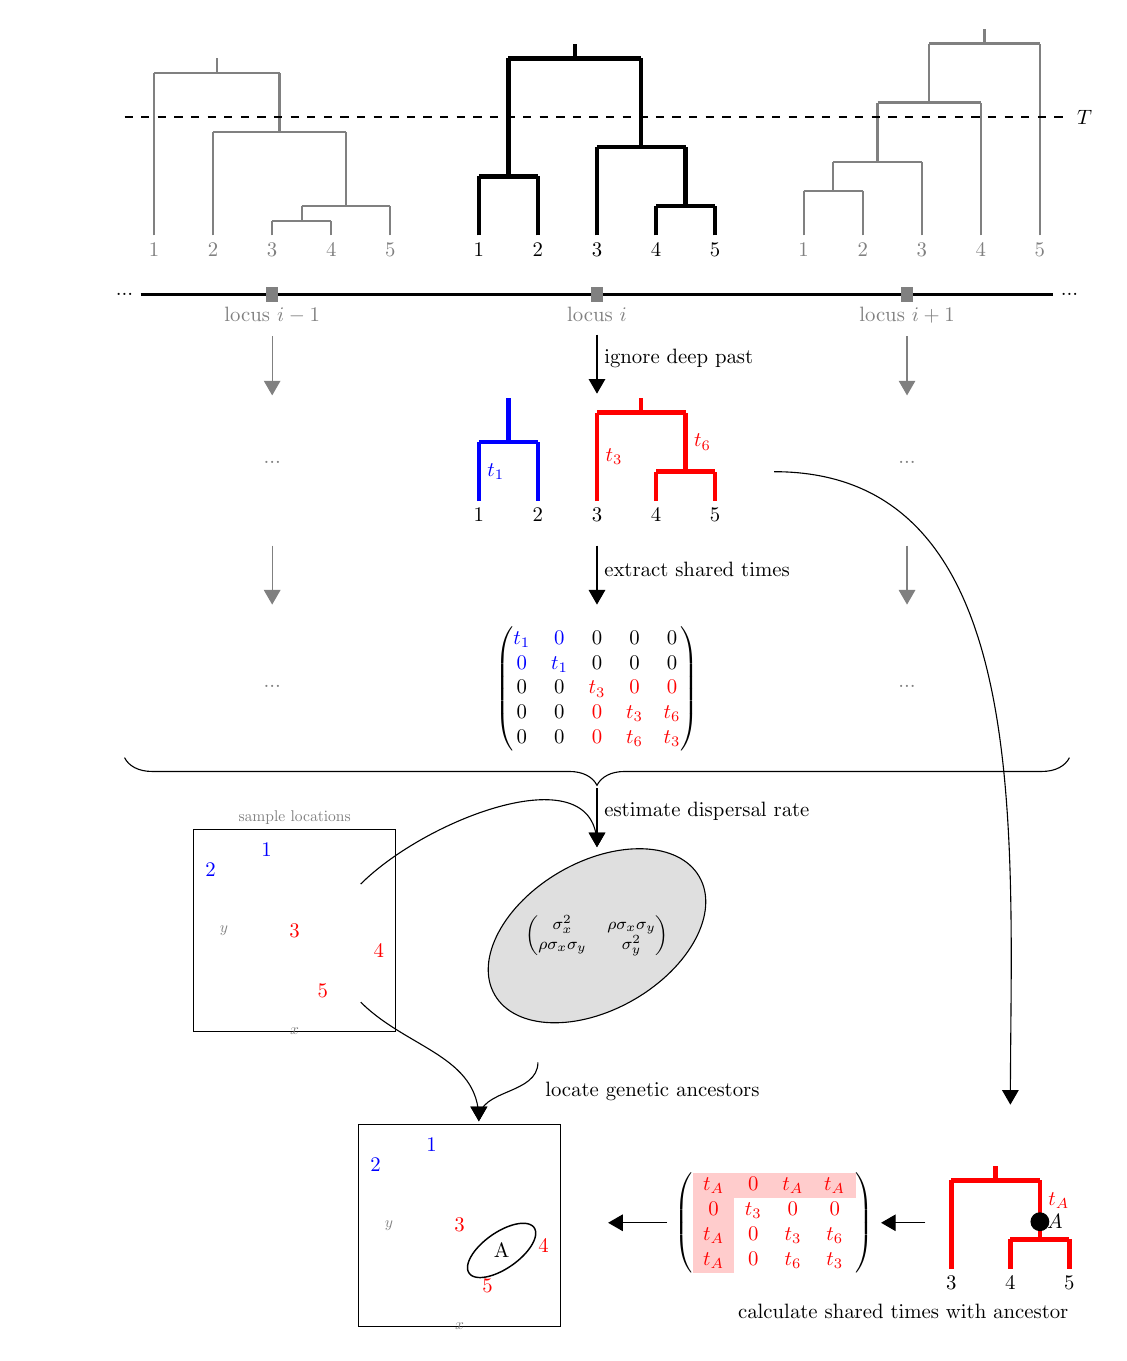
\begin{tikzpicture}[>=triangle 60, scale=0.75, every node/.style={scale=0.75}] %if figure too big, adjust both scales equally

%%%%%%%%%%
%tree sequence
%%%%%%%%%%

%%%%%%%%%%%%%%%
%genome
  \node[] (gleft) at (-8,-1) {...};
  \node[] (gright) at (8,-1) {...};
  \draw[thick] (gleft) -- (gright);

%%%%%%%%%%%%%%
%focal tree
  
  %location on genome
  \coordinate (tree) at (0,0);
  \draw[line width=2mm, gray] (-0.1,-1) -- (0.1,-1) node[midway, below] (locus) {locus $i$};
  
  % sample nodes
  \foreach \n in {1,...,5}{
    \coordinate (n\n) at (\n - 3, 0); % define coordinate
    \node[below = 0cm of n\n] {\n}; %node label
  }
  % ancestor node 1
  \foreach \t in {0.5}{
    \foreach \n in {4,5}{
      \draw[ultra thick] (n\n) -- (n\n |- 0,\t);
    }
  \draw[ultra thick] (n4 |- 0,\t) -- (n5 |- 0,\t) coordinate[midway] (n6);
  }    
  % ancestor node 2
  \foreach \t in {1}{ %coalescent time
    \foreach \n in {1,2}{ %nodes that coalesce
      \draw[ultra thick] (n\n) -- (n\n |- 0,\t);
    }
  \draw[ultra thick] (n1 |- 0,\t) -- (n2 |- 0,\t) coordinate[midway] (n7);
  }
  % ancestor node 3
  \foreach \t in {1.5}{
    \foreach \n in {3,6}{
      \draw[ultra thick] (n\n) -- (n\n |- 0,\t);
    }
  \draw[ultra thick] (n3 |- 0,\t) -- (n6 |- 0,\t) coordinate[midway] (n8);
  }  
  % ancestor node 4
  \foreach \t in {3}{
    \foreach \n in {7,8}{
      \draw[ultra thick] (n\n) -- ( n\n |- 0,\t );
    }
  \draw[ultra thick] ( n7 |- 0,\t ) -- ( n8 |- 0,\t ) coordinate[midway] (n9);
  }
  % mrca stem
  \draw[ultra thick] (n9) -- (n9 |- 0,3.25);      
 
 %%%%%%%%%%%%%%
 %left tree
  
  %location on genome
  \coordinate (tree) at (0,0);
  \draw[line width=2mm, gray] (-5.6, -1) -- (-5.4, -1) node[midway, below] (llocus) {locus $i-1$};
  
  % sample nodes
  \foreach \n in {1,...,5}{
    \coordinate (n\n) at (-6.5 + \n - 2, 0); % define coordinate
    \node[below = 0cm of n\n, gray] {\n}; %node label
  }
  % ancestor node 1
  \foreach \t in {0.25}{
    \foreach \n in {3,4}{
      \draw[thick, gray] (n\n) -- (n\n |- 0,\t);
    }
  \draw[ thick, gray] (n3 |- 0,\t) -- (n4 |- 0,\t) coordinate[midway] (n6);
  }    
  % ancestor node 2
  \foreach \t in {0.5}{ %coalescent time
    \foreach \n in {6,5}{ %nodes that coalesce
      \draw[ thick, gray] (n\n) -- (n\n |- 0,\t);
    }
  \draw[ thick, gray] (n6 |- 0,\t) -- (n5 |- 0,\t) coordinate[midway] (n7);
  }
  % ancestor node 3
  \foreach \t in {1.75}{
    \foreach \n in {2,7}{
      \draw[ thick, gray] (n\n) -- (n\n |- 0,\t);
    }
  \draw[ thick, gray] (n2 |- 0,\t) -- (n7 |- 0,\t) coordinate[midway] (n8);
  }  
  % ancestor node 4
  \foreach \t in {2.75}{
    \foreach \n in {1,8}{
      \draw[ thick, gray] (n\n) -- ( n\n |- 0,\t );
    }
  \draw[thick, gray] ( n1 |- 0,\t ) -- ( n8 |- 0,\t ) coordinate[midway] (n9);
  }
  % mrca stem
  \draw[thick, gray] (n9) -- (n9 |- 0,3); 
  
%%%%%%%%%%%%%%
 %right tree
  
  %location on genome
  \coordinate (tree) at (0,0);
  \draw[line width=2mm, gray] (5.15,-1) -- (5.35,-1) node[midway, below] (rlocus){locus $i+1$};
%  
  % sample nodes
  \foreach \n in {1,...,5}{
    \coordinate (n\n) at (5.5 + \n - 3, 0); % define coordinate
    \node[below = 0cm of n\n, gray] {\n}; %node label
  }
  % ancestor node 1
  \foreach \t in {0.75}{
    \foreach \n in {1,2}{
      \draw[ thick, gray] (n\n) -- (n\n |- 0,\t);
    }
  \draw[ thick, gray] (n1 |- 0,\t) -- (n2 |- 0,\t) coordinate[midway] (n6);
  }    
  % ancestor node 2
  \foreach \t in {1.25}{ %coalescent time
    \foreach \n in {6,3}{ %nodes that coalesce
      \draw[ thick, gray] (n\n) -- (n\n |- 0,\t);
    }
  \draw[ thick, gray] (n6 |- 0,\t) -- (n3 |- 0,\t) coordinate[midway] (n7);
  }
  % ancestor node 3
  \foreach \t in {2.25}{
    \foreach \n in {7,4}{
      \draw[ thick, gray] (n\n) -- (n\n |- 0,\t);
    }
  \draw[ thick, gray] (n7 |- 0,\t) -- (n4 |- 0,\t) coordinate[midway] (n8);
  }  
  % ancestor node 4
  \foreach \t in {3.25}{
    \foreach \n in {8,5}{
      \draw[ thick, gray] (n\n) -- ( n\n |- 0,\t );
    }
  \draw[thick, gray] ( n8 |- 0,\t ) -- ( n5 |- 0,\t ) coordinate[midway] (n9);
  }
  % mrca stem
  \draw[thick, gray] (n9) -- (n9 |- 0,3.5); 
  
%%%%%%%%%%%%%%%%%
%time cut off
  \draw[thick, dashed] ($(gleft) + (0,3)$) -- ($(gright) + (0,3)$) node[right] {$T$};

%%%%%%%%%%%%
% down arrows
\draw[->] (locus.south) -- ($(locus.south) + (0,-1)$) node[midway, right, yshift=0.1cm] {ignore deep past};
\draw[->, gray] (llocus.south) -- ($(llocus.south) + (0,-1)$) node[below, yshift=-1cm] {...};
\draw[->, gray] (rlocus.south) -- ($(rlocus.south) + (0,-1)$) node[below, yshift=-1cm] {...};

%%%%%%%%%%%%%
%subtrees
%%%%%%%%%%%

  % sample nodes
  \foreach \n in {1,...,5}{
    \coordinate (n\n) at (\n - 3, -4.5); % define coordinate
    \node[below = 0cm of n\n] {\n}; %node label
  }
  % ancestor node 1
  \foreach \t in {-4}{
    \foreach \n in {4,5}{
      \draw[ultra thick, red] (n\n) -- (n\n |- 0,\t);
    }
  \draw[ultra thick, red] (n4 |- 0,\t) -- (n5 |- 0,\t) coordinate[midway] (n6);
  }
  % ancestor node 2
  \foreach \t in {-3.5}{ %coalescent time
%    \foreach \n in {1,2}{ %nodes that coalesce
%      \draw[ultra thick] (n\n) -- (n\n |- 0,\t);
%    }
  \draw[ultra thick, blue] (n1) -- (n1 |- 0,\t)  node[midway, right] {$t_1$}; 
  \draw[ultra thick, blue] (n2) -- (n2 |- 0,\t); 
  \draw[ultra thick, blue] (n1 |- 0,\t) -- (n2 |- 0,\t) coordinate[midway] (n7);
  }
  % ancestor node 3
  \foreach \t in {-3}{
    \foreach \n in {3,6}{
      \draw[ultra thick, red] (n\n) -- (n\n |- 0,\t) node[midway, right] {$t_\n$};
    }
  \draw[ultra thick, red] (n3 |- 0,\t) -- (n6 |- 0,\t) coordinate[midway] (n8);
  }  
  % blue mrca stem
  \draw[ultra thick, blue] (n7) -- (n7 |- 0,-2.75); 
  % red mrca stem
  \draw[ultra thick, red] (n8) -- (n8 |- 0,-2.75); 
  
%  \node[gray] at (1,-6) {subtree $j$};  

% down arrows
\draw[->] ($(n3.south) + (0,-0.75)$) -- ($(n3.south) + (0,-1.75)$) node[midway, right, yshift=0.1cm] {extract shared times};
\draw[->, gray] ($(n3.south) + (-5.5,-0.75)$) -- ($(n3.south) + (-5.5,-1.75)$) node[below, yshift=-1.25cm] {...};
\draw[->, gray] ($(n3.south) + (5.25,-0.75)$) -- ($(n3.south) + (5.25,-1.75)$) node[below, yshift=-1.25cm] {...};

%%%%%%%%%%%%
%shared times
%%%%%%%%%%%

  \node[anchor = north] (matrix) at ($(n3.south) + (0,-2)$) {
   $\begin{pmatrix} 
        \color{blue}{t_1} & \color{blue}{0} & \color{black}{0} & \color{black}{0} & \color{black}{0} \\
        \color{blue}{0} & \color{blue}{t_1} & \color{black}{0}& \color{black}{0} & \color{black}{0} \\
        \color{black}{0} & \color{black}{0} & \color{red}{t_3} & \color{red}{0} & \color{red}{0} \\ 
        \color{black}{0} & \color{black}{0} & \color{red}{0} & \color{red}{t_3} & \color{red}{t_6} \\ 
        \color{black}{0} & \color{black}{0} & \color{red}{0} & \color{red}{t_6} & \color{red}{t_3} 
  \end{pmatrix}$
  };

% down arrows
\draw[decoration={brace,raise=5pt,amplitude=10pt,mirror},decorate] ($(matrix.south) + (gleft) + (0,1.25)$) -- ($(matrix.south) + (gright) + (0,1.25)$);
\coordinate(A) at ($(matrix.south) + (0, -1.5)$);
\draw[->] ($(matrix.south) + (0, -0.5)$) -- (A) node[midway, right, yshift=0.1cm] {estimate dispersal rate};

%%%%%%%%%%%%%%
%dispersal rate
%%%%%%%%%%%%%%

\node[anchor=north] at ($(matrix.south) + (gleft) + (0, -3.5)$) (locations) {
  \begin{axis}[
      title=sample locations,
      title style={at={(axis description cs:0.5,0.95)}, gray},
      cycle list name=black white,
      height=5cm,
      width=5cm,
      xlabel=$x$,
      ylabel=$y$,
      samples=5,
      domain=0:1,
      ymin = 0,
      ymax = 1,
      ticks=none,
      x label style={at={(axis description cs:0.5,0)}, anchor=center, color=gray},
      y label style={at={(axis description cs:0.15,0.5)},rotate=-90,anchor=center, color=gray}
  ]
%  \addplot+[only marks]  {rand}; %plot some random locations
    \addplot[only marks, mark=text, text mark = {1}, blue] table { 
      0.4 0.9
    };
    \addplot[only marks, mark=text, text mark = {2}, blue] table { 
      0.3 0.8
    };
    \addplot[only marks, mark=text, text mark = {3}, red] table { 
      0.45 0.5
    };
    \addplot[only marks, mark=text, text mark = {4}, red] table { 
      0.6 0.4
    };    
    \addplot[only marks, mark=text, text mark = {5}, red] table { 
      0.5 0.2
    };    
  \end{axis}
};

\draw[->] ($(locations) + (4cm, 2.5cm)$) to [out=45, in=90] (A);

\coordinate(A) at ($(matrix.south) + (0, -3)$);
\draw[fill=lightgray!50!white, rotate around={30:(A)}] (A) ellipse (2cm and 1.25cm);
  \node[] at (A) {
  \footnotesize
%   $\widehat{\mathbf{\Sigma}}$
    $\begin{pmatrix} 
      \sigma_x^2 & \rho\sigma_x\sigma_y \\
      \rho\sigma_x\sigma_y & \sigma_y^2
    \end{pmatrix}$
  };

% down arrows
\coordinate(A) at (-2,-15);
\draw[->] ($(A)+(1,1)$) to [out=270, in=90] node[midway, right, xshift=0.5cm] {locate genetic ancestors} (A) ;
\draw[->] ($(locations) + (4cm, 0.5cm)$) to [out=315, in=90] (A);

%%%%%%%%%%%%
% locate ancestors
%%%%%%%%%%%%%

% red tree
\begin{scope}[xshift = 6cm, yshift = -13cm]

  % sample nodes
  \foreach \n in {3,...,5}{
    \coordinate (n\n) at (\n - 3, -4.5); % define coordinate
    \node[below = 0cm of n\n] {\n}; %node label
  }
  % ancestor node 1
  \foreach \t in {-4}{
    \foreach \n in {4,5}{
      \draw[ultra thick, red] (n\n) -- (n\n |- 0,\t);
    }
  \draw[ultra thick, red] (n4 |- 0,\t) -- (n5 |- 0,\t) coordinate[midway] (n6);
  }    
  % ancestor node 3
  \foreach \t in {-3}{
    \foreach \n in {3,6}{
      \draw[ultra thick, red] (n\n) -- (n\n |- 0,\t);
    }
  \draw[ultra thick, red] (n3 |- 0,\t) -- (n6 |- 0,\t) coordinate[midway] (n8);
  }
  % red mrca stem
  \draw[ultra thick, red] (n8) -- (n8 |- 0,-2.75); 
  % focal ancestor
  \draw[ultra thick, red] (n6 |- 0,-3.7) -- (n6 |- 0,-3) node[midway, right, red] {$t_A$};  
  \draw[fill=black] (n6 |- 0,-3.7) circle (0.15cm) node[right] {$A$};

\end{scope}

% shared times
  \node[anchor = north] (matrix) at (3,-15.75) {
   $\left(\begin{array}{>{\columncolor{red!20}}cccc}
        \rowcolor{red!20}
        \color{red}{t_A} & \color{red}{0} & \color{red}{t_A} & \color{red}{t_A} \\ 
        \color{red}{0} & \color{red}{t_3} & \color{red}{0} & \color{red}{0} \\ 
        \color{red}{t_A} & \color{red}{0} & \color{red}{t_3} & \color{red}{t_6} \\ 
        \color{red}{t_A} & \color{red}{0} & \color{red}{t_6} & \color{red}{t_3} 
  \end{array}\right)$
  };

% ancestor plot
\node[anchor=east] at ($(matrix.west) + (-4.75, -1.75)$) (locations) {
  \begin{axis}[
      cycle list name=black white,
      height=5cm,
      width=5cm,
      xlabel=$x$,
      ylabel=$y$,
      samples=5,
      domain=0:1,
      ymin = 0,
      ymax = 1,
      ticks=none,
      x label style={at={(axis description cs:0.5,0)}, anchor=center, color=gray},
      y label style={at={(axis description cs:0.15,0.5)},rotate=-90,anchor=center, color=gray}
  ]
%  \addplot+[only marks]  {rand}; %plot some random locations
    \addplot[only marks, mark=text, text mark = {1}, blue] table { 
      0.4 0.9
    };
    \addplot[only marks, mark=text, text mark = {2}, blue] table { 
      0.3 0.8
    };
    \addplot[only marks, mark=text, text mark = {3}, red] table { 
      0.45 0.5
    };
    \addplot[only marks, mark=text, text mark = {4}, red] table { 
      0.6 0.4
    };    
    \addplot[only marks, mark=text, text mark = {5}, red] table { 
      0.5 0.2
    };    
    \addplot[mark=text, text mark = {A}, black] table { 
      0.525 0.375
    };
%    \addplot[domain=0:360,data cs=polar, samples=200, line width=0.7pt, red] (x,{1/(sqrt(1 - 2*cos(x)*cos(x)))});
\addplot [domain=-pi:pi, samples=200, black, line width=0.7pt, rotate around={35:(axis cs:0.525,0.375)}] ({0.525 + sqrt(0.005)*sin(deg(x))}, {0.375 + sqrt(0.008)*cos(deg(x))});
  \end{axis}
};

%arrows
\draw[->] (3,-4) to [out=0, in=90, looseness=1] ($(matrix) + (4,2)$);
\draw[->] ($(matrix.east) + (0.75,0)$) -- (matrix.east) node[midway, below, yshift=-1.25cm] {calculate shared times with ancestor};
\draw[->] (matrix.west) -- ($(matrix.west) + (-1,0)$);

\end{tikzpicture}
\end{center}

%%%%%%%%%%%%%%%%%%%%%%%%%%%%%%%%%%%%%%%%%%%%%%%%%
  \caption{
  (Continued on the following page.)
}
\label{fig:overview}
\end{figure}
%\clearpage
\begin{figure}[!t]
  \contcaption{
  \textbf{Conceptual overview of the approach.}
From a sequence of trees covering the full genome, we downsample to trees at approximately unlinked loci.
To avoid the influence of strongly non-Brownian dynamics at deeper times (e.g., glacial refugia, boundaries), we ignore times deeper than $T$, which divides each tree into multiple subtrees (here, blue and red subtrees at locus $i$).
From these subtrees we extract the shared evolutionary times of each lineage with all others.
In practice (but not shown here), we use multiple samples of the tree at a given locus, for importance sampling, and also extract the coalescence times for importance sample weights. 
Under Brownian motion, the shared times describe the covariance we expect to see in the locations of our samples, and so using the times and locations we can find maximum likelihood dispersal rate (a 2x2 covariance matrix).
While we can estimate a dispersal rate at each locus, a strength of our approach is that we combine information across many loci, by multiplying likelihoods, to estimate genome-wide (or per-chromosome) dispersal rates. 
In practice (but not shown here), we estimate dispersal in multiple epochs, which allows for variation in dispersal rate over time and helps absorb non-Brownian movements further in the past.
Finally, we locate a genetic ancestor at a particular locus (a point on a tree, here $A$) by first calculating the time this ancestor shares with each of the samples in its subtree, and then using this matrix and the dispersal rate to calculate the probability distribution of the ancestor's location conditioned on the sample locations.
In practice (but not shown here), we calculate the locations of ancestors of a given sample at a given time at many loci, combining information across loci into a distribution of genome-wide ancestry across space.
  }% Continued caption
\end{figure}

%%%%%%%%%%%%%%%%%%%%%%%%%%%%%%%%%%%%%%%%%%%%%%%%%

The rate of dispersal, which determines the average distance between parents and offspring, is a key parameter in ecology and evolution.
To estimate this parameter we assume that in each generation the displacement of an offspring from its mother is normally distributed with a mean of 0 and covariance matrix $\mathbf{\Sigma}$.
The covariance matrix is determined by the standard deviations $\sigma_{x}$ and $\sigma_{y}$ along the x (longitudinal) and y (latitudinal) axes, respectively, as well as the correlation, $\rho$, in displacements between these two axes.
The average distance between mothers and offspring is then $\sqrt{2/\pi} \sigma_i$ in each dimension.
We refer to the covariance matrix $\mathbf{\Sigma}$ as the (per-generation) dispersal rate.

Given this model, the path of a lineage from its ancestral location to the present day location is described by a Brownian motion. 
Lineages covary in their locations because of shared evolutionary histories -- lineages with a more recent common ancestor covary more.
Given a tree at a locus we can calculate the covariance matrix of shared evolutionary times and compute the likelihood of the dispersal rate, $\mathbf{\Sigma}$, which is normally distributed given this covariance matrix (Equation \eqref{eq:PS}).
At each locus we can estimate the likelihood of the dispersal rate given the tree at that locus and, given we sample loci far enough apart that they are essentially independent, multiply likelihoods across loci to derive a genome-wide likelihood, and thus a genome-wide maximum likelihood dispersal rate.

Under this same model we can also estimate the locations of genetic ancestors at a locus.
Any point along a tree at any locus is a genetic ancestor of one or more current day samples. 
This ancestor's lineage has dispersed away from the location of the most recent common ancestor of the sample, and covaries with current day samples in their geographic location to the extent that it shares times in the tree with them.
Under this model, the location of an ancestor is influenced by the locations of all samples in the same tree, including those that are not direct descendants \citep[cf.][]{wohns2021unified}.
For example, in Figure \ref{fig:overview} the ancestor's location is not be the midpoint of its two descendants (samples 4 and 5); the ancestor's location is also pulled towards sample 3 since the ancestor and sample 3 both arose from a common ancestor.
Conditioning on the sample locations, and given the shared times and previously inferred dispersal rate, we can compute the probability the ancestor was at any location, which again is a normal distribution (Equation \eqref{eq:PsaCentered}). 
In contrast to dispersal, for ancestral locations we do not want to multiply likelihoods across loci since the ancestors at distant loci are likely distinct.
Instead we calculate the maximum likelihood location of genetic ancestors at each locus to get a cloud of likely ancestral locations, and use these clouds to visualize the spatial spread of ancestry backwards through time.

We estimate marginal trees along the genome using \texttt{Relate} \citep{speidel2019method}. 
Relate infers a sequence of tree topologies and associated branch lengths, and can return a set of posterior draws of the branch lengths on a given tree. 
This posterior distribution of branch lengths is useful to us as the shared times in the tree are key to the amount of time that individual lineages have had to disperse away from one another and we wish include uncertainty in the times into our method. 
Relate gives us a posterior distribution of branch lengths that is estimated using a coalescent prior, which assumes a panmictic population of varying population size (the size changes are estimated as part of the method), where any two lineages are equally likely to coalesce. 
This panmictic prior results in a bias in the coalescent times under a spatial model, where geographically proximate samples are more likely to coalesce. 
To correct for this bias we make use of importance sampling to weight the samples of branch lengths at each locus.  
We then calculate the weighted average likelihood over our draws of our sample of trees at a locus (or loci), so that it is as if they were drawn from a prior of branching Brownian motion \citep{meligkotsidou2007postprocessing}. 
Branching Brownian motion, also known as the Brownian-Yule process, is a simple model of spatial genealogies in a continuous population; it does not describe the full complexities of spatial models such as the spatial coalescent, but it provides an analytically tractable model and a reasonable approximation over short-time scales \citep{edwards1970estimation,rannala1996probability,meligkotsidou2007postprocessing,novembre2009likelihood}.

In practice we concentrate on the recent past history of our sample. 
For our estimates of dispersal rates in particular we do not want to assume that our model of Gaussian dispersal (and branching Brownian motion) holds deep into the past history of the sample. 
This is because the long-term movement of lineages is constrained by geographic barriers (e.g., oceans) and larger scale population movements may erase geographic signals over deep time scales. 
On theoretical level ignoring the deep past may also be justified because in a finite habitat the locations of coalescence events further back in time become independent of sampling locations as lineages have moved around sufficiently \citep{wilkins2002coalescent}. 
Thus we only use this geographic model to some time point in the past ($T$), and at each locus we use the covariance of shared branch lengths based on the set of subtrees formed by cutting off the full tree $T$ generations back. 

To relax the assumption of a constant dispersal rate we extend our method to estimate dispersal rates in multiple epochs. 
Under Brownian motion this extension is fairly straight-forward as the covariance in sample locations is simply the sum, across epochs, of epoch-specific covariances (the Kronecker product of the shared times in a epoch and the dispersal rate in that epoch).
An added benefit of estimating dispersal in epochs is that the estimates in more distant epochs can absorb some of the non-Brownian dynamics further back in time, increasing the accuracy of estimates in more recent epochs.

%%%%%%%%%%%%%%%%%%%%%%%%%%%%%%%%%%%%%%%%%%%%%%%%%
\subsection*{Simulations}
%%%%%%%%%%%%%%%%%%%%%%%%%%%%%%%%%%%%%%%%%%%%%%%%%

We first wanted to test the performance of our method in a situation where the true answers were known.
To do this we used a combination of spatially-explicit forward-time simulations \citep{haller2019slim}, coalescent simulations \citep{kelleher2016efficient}, and tree-sequence tools \citep{haller2019tree,kelleher2019inferring,speidel2019method} to compare our estimates of dispersal rates and ancestor locations with the truth (see \nameref{sec:methods}).
This was also an opportunity to compare our estimates using the true trees vs.\ the Relate-inferred trees, to examine the influence of errors in tree inference.

%%%%%%%%%%%%%%%%%%%%%%%%%%%%%%%%%%%%%%%%%%%%%%%%%
\subsubsection*{Dispersal rates}

Our method does a good job at capturing the simulated dispersal rate when using the true trees, especially at lower dispersal rates (Figure \ref{fig:sims}A). 
At larger dispersal rates the true trees tend to cause underestimates of the simulated dispersal rate, likely a consequence of the finite habitat we simulate (with reflecting boundaries). 
Here we use a time cutoff of only $100$ generations in a 50x50 habitat, meaning that with any dispersal rate larger than $\sigma^2 \sim 50^2/100 = 5^2$ a lineage is reasonably likely to cross the entire habitat in that time.
At higher dispersal rates or longer cutoff times (Figure \ref{fig:sup_sigma_corr_tcut}), the simple Brownian motion model expects the samples to be more broadly distributed than the finite habitat allows, leading to larger underestimates.
Regardless, we can interpret the dispersal rate inferred from the true trees as a true `effective' dispersal rate, given the boundaries, local competition, biparental reproduction, etc. 
Encouragingly, the estimates from the inferred trees are highly correlated with these estimates, although with an upward bias.
This upward bias is expected given the combination of isolation-by-distance and errors in inferring tree topologies, causing geographically distant samples to be mistakenly inferred to be close relatives.
The bias (and variance across replicates) increases when we just use the panmictic coalescent prior from \texttt{Relate} (Figure \ref{fig:sup_sigma_imp}), showing that our spatial prior implemented via importance sampling improves our inference.

%%%%%%%%%%%%%%%%%%%%%%%%%%%%%%%%%%%%%%%%%%%%%%%%%
%simulation figure%
%%%%%%%%%%%%%%%%%%%%%%%%%%%%%%%%%%%%%%%%%%%%%%%%%

\begin{figure}[!b]
%\captionsetup{labelformat=empty}
\begin{center}
\begin{tikzpicture}[remember picture]

  % 1 epoch dispersal mcles
  \node[] (sigmax-corr) {
    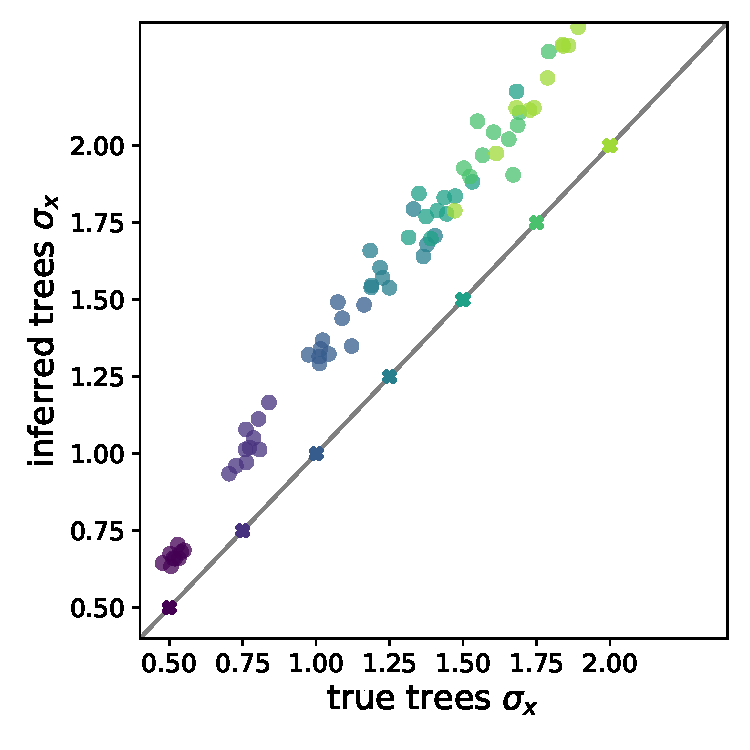
\includegraphics[height=0.32\linewidth, trim = {0cm 0 0cm 0}, clip]{plots/sim_sigmax_5numiter_100tCutoff.pdf}    
  };
  \node[left = 0cm of sigmax-corr.north west, anchor = north west, yshift = -0.15cm] (A) {
    \textbf{A}
  };

  % 2 epoch dispersal mcles: small -> large
  \node[right = -0.2cm of sigmax-corr] (sigmax-corr-2epoch) {
    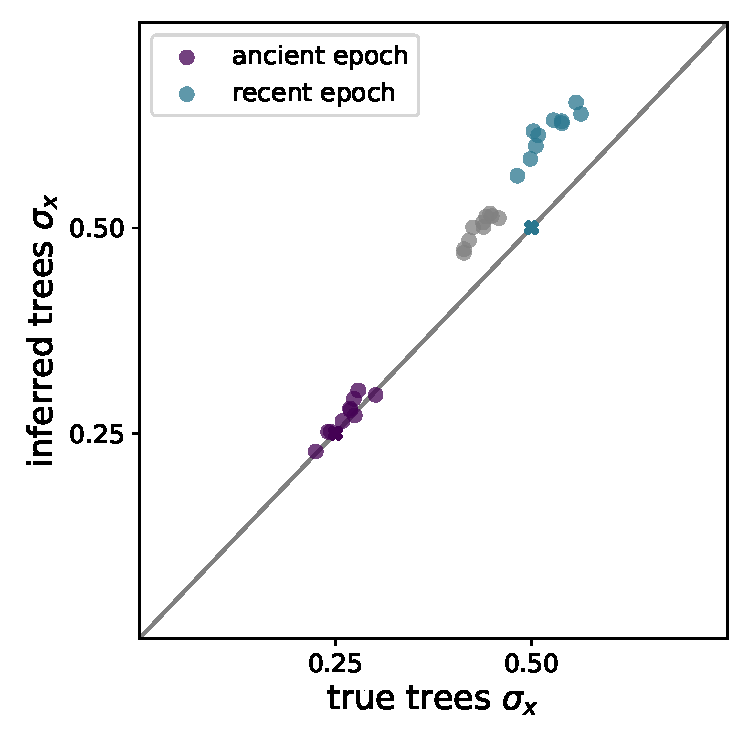
\includegraphics[height=0.32\linewidth, trim = {0cm 0 0cm 0}, clip]{plots/sim_2epoch_mcles_tsplits[0.25, 0.5].pdf}
  };
  \node[left = 0cm of sigmax-corr-2epoch.north west, anchor = north west, yshift = -0.15cm] (B) {
    \textbf{B}
  };

  % 2 epoch dispersal mcles: large -> small
  \node[right = -0.2cm of sigmax-corr-2epoch] (sigmax-corr-2epoch-2) {
    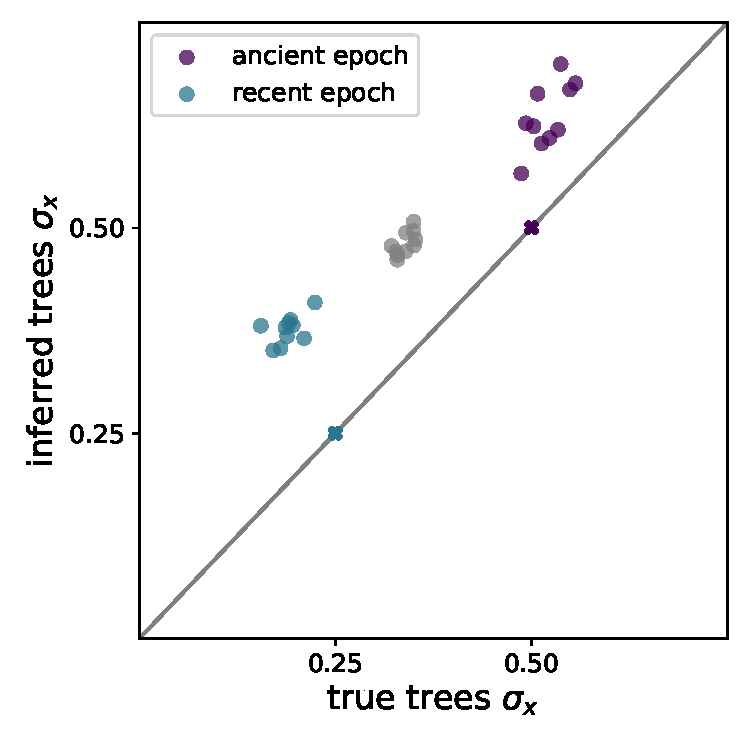
\includegraphics[height=0.32\linewidth, trim = {0cm 0 0cm 0}, clip]{plots/sim_2epoch_mcles_tsplits[0.5, 0.25].pdf}
  };
  \node[left = 0cm of sigmax-corr-2epoch-2.north west, anchor = north west, yshift = -0.15cm] (C) {
    \textbf{C}
  };

  % RMSE
  \node[below = -0.6cm of sigmax-corr.south west, anchor = north west] (RMSE) {
    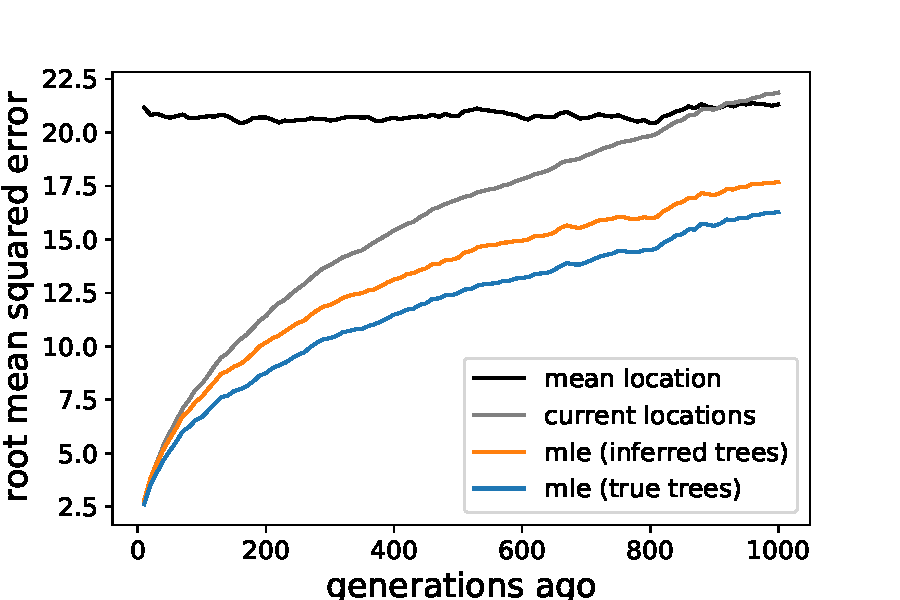
\includegraphics[height=0.25\linewidth, trim = {0cm 0 0.75cm 0cm}, clip]{plots/rmse_5numiter.pdf}
  };
  \node[left = 0cm of RMSE.north west, anchor = north west, yshift = -0.05cm] (D) {
    \textbf{D}
  };  

  % confidence ellipses
  \node[right = -0.5cm of RMSE, yshift=-0.1cm] (CI-1) {
    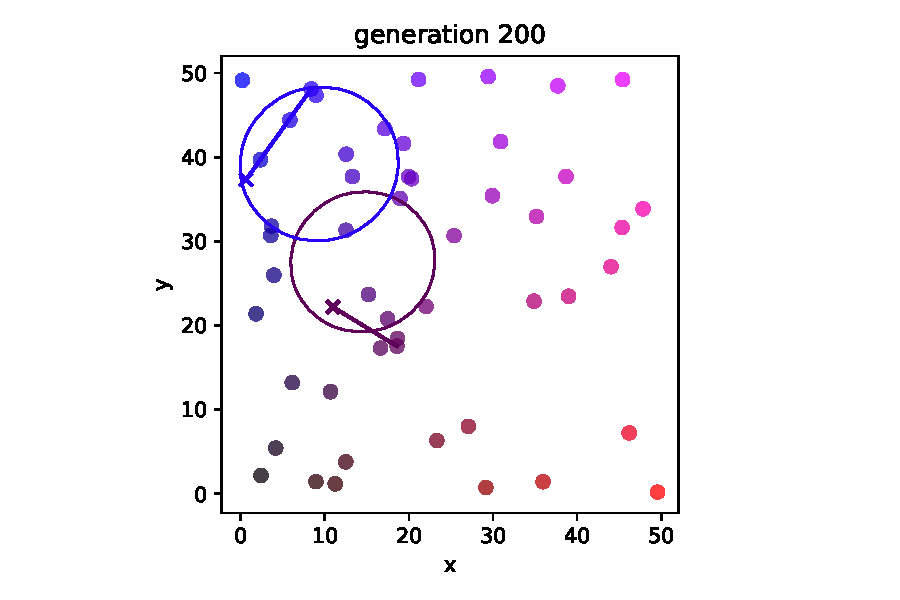
\includegraphics[height=0.25\linewidth, trim = {2.5cm 0 0cm 0}, clip]{plots/CIs-coalesce-true_trees_time200.pdf}
  };
  \node[right = -1.5cm of CI-1] (CI-2) {
    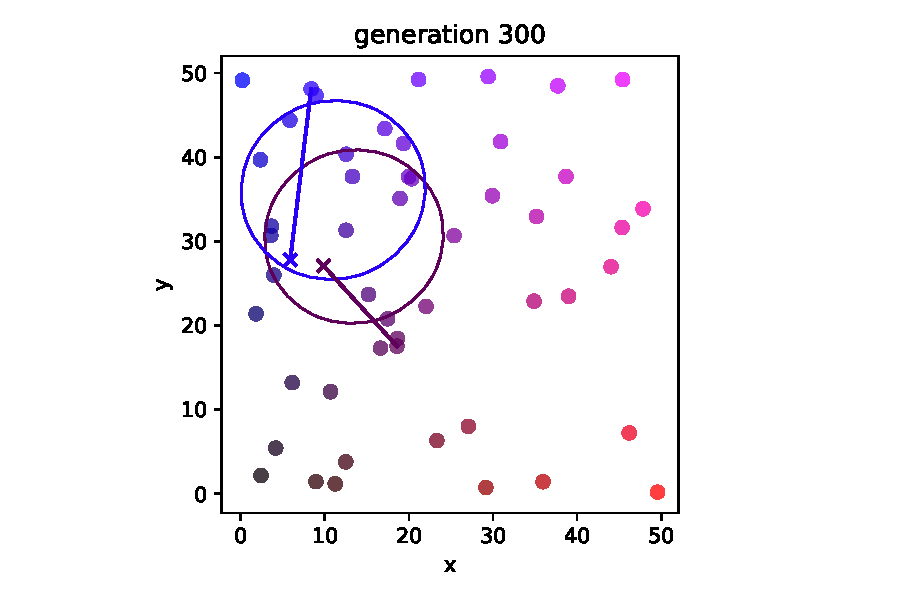
\includegraphics[height=0.25\linewidth, trim = {3.5cm 0 0cm 0}, clip]{plots/CIs-coalesce-true_trees_time300.pdf}
  };
  \node[right = -1.5cm of CI-2] (CI-3) {
    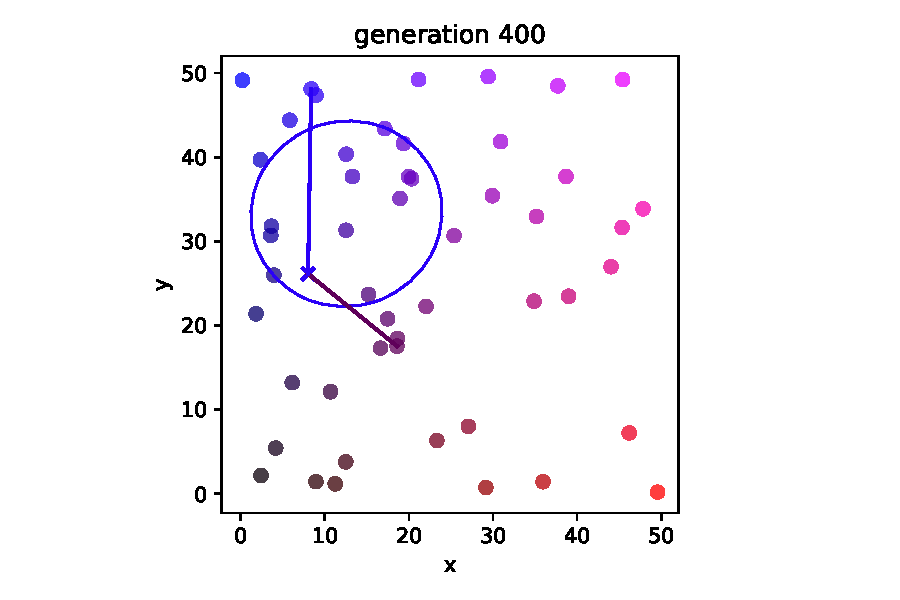
\includegraphics[height=0.25\linewidth, trim = {3.5cm 0 0cm 0}, clip]{plots/CIs-coalesce-true_trees_time400.pdf}
  };  
  \node[above left = 0cm of CI-1.north west, anchor = north west, yshift = 0.05cm] (E) {
    \textbf{E}
  };

  % mean RMSE
  \node[below = -0.5cm of RMSE] (RMSE-mean) {
    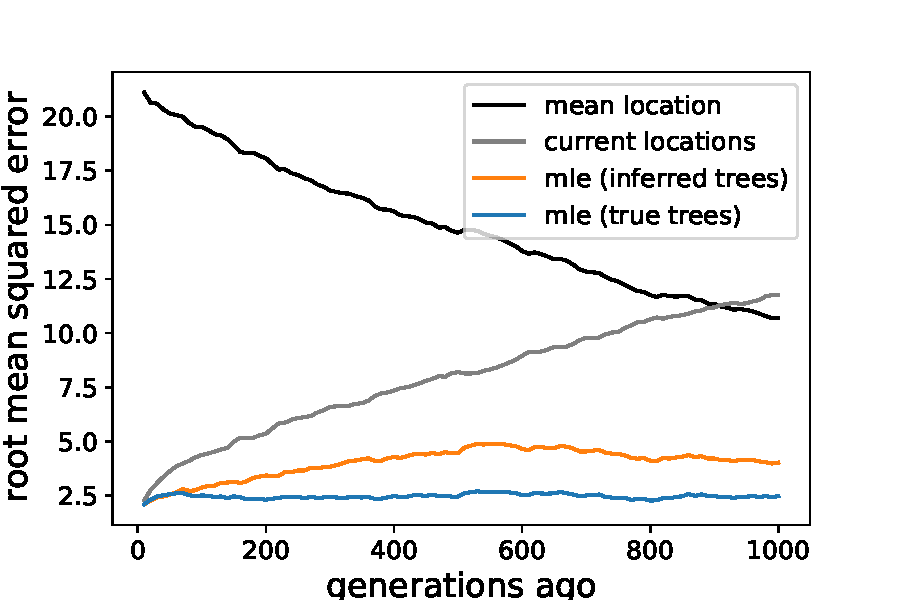
\includegraphics[height=0.25\linewidth, trim = {0cm 0 0.75cm 0cm}, clip]{plots/rmse_mean_5numiter.pdf}
  };
  \node[left = 0cm of RMSE-mean.north west, anchor = north west, yshift = -0.05cm] (F) {
    \textbf{F}
  };  

  % MLEs
  \node[below = -0.5cm of CI-1] (BLUP-1) {
    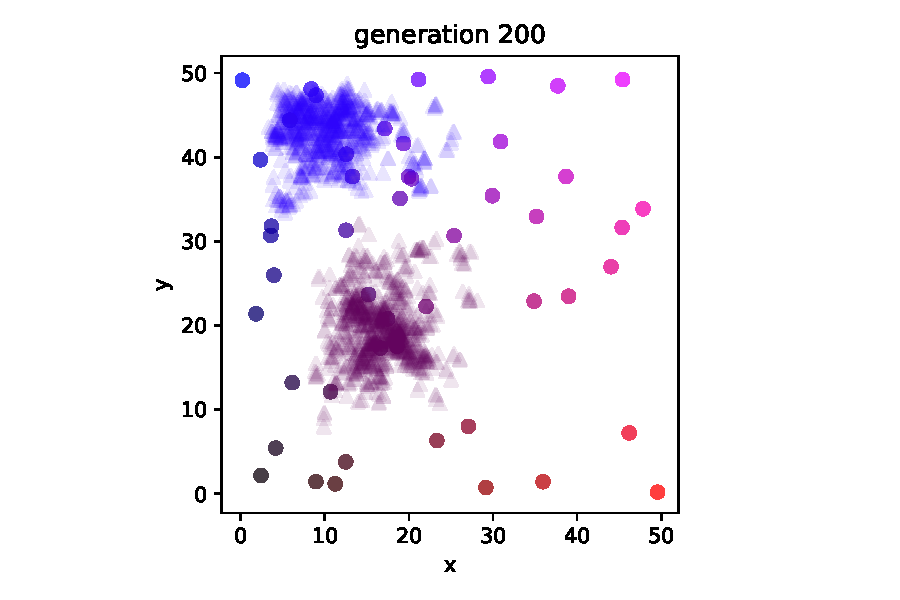
\includegraphics[height=0.25\linewidth, trim = {2.5cm 0 0cm 0}, clip]{plots/BLUPs-coalesce-true_trees_time200.pdf}
  };
  \node[below = -0.5cm of CI-2] (BLUP-2) {
    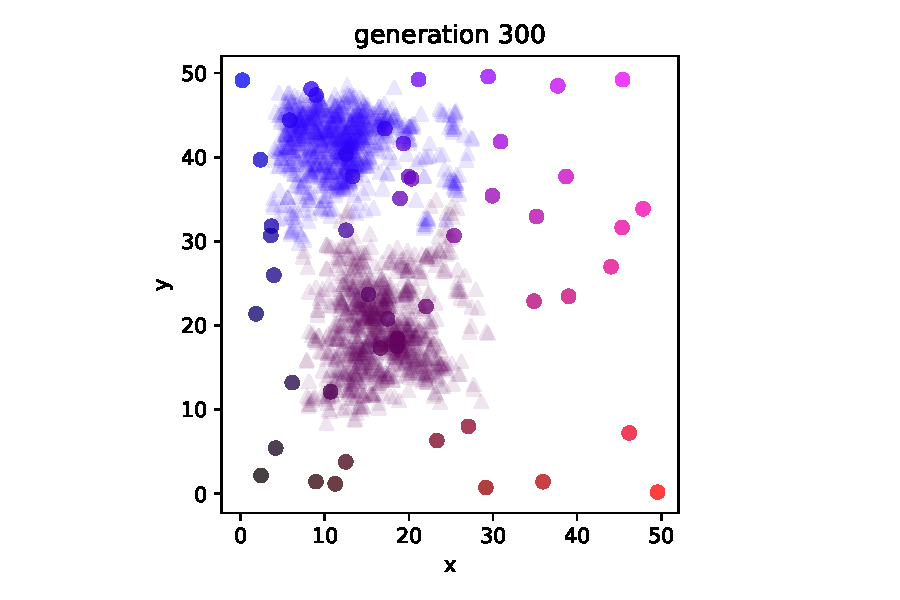
\includegraphics[height=0.25\linewidth, trim = {3.5cm 0 0cm 0}, clip]{plots/BLUPs-coalesce-true_trees_time300.pdf}
  };
  \node[below = -0.5cm of CI-3] (BLUP-3) {
    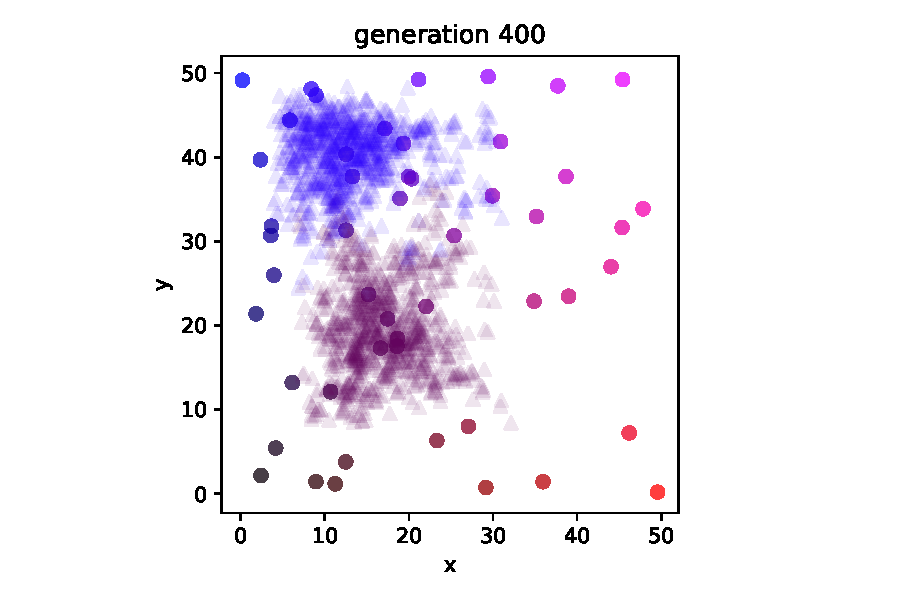
\includegraphics[height=0.25\linewidth, trim = {3.5cm 0 0cm 0}, clip]{plots/BLUPs-coalesce-true_trees_time400.pdf}
  };  
  \node[above left = 0cm of BLUP-1.north west, anchor = north west, yshift = 0.05cm] (G) {
    \textbf{G}
  };

\end{tikzpicture}  
\end{center}
%%%%%%%%%%%%%%%%%%%%%%%%%%%%%%%%%%%%%%%%%%%%%%%%%
%\caption{}
%\end{figure}
%%\clearpage
%\begin{figure}[!t]
%  \ContinuedFloat
%  \caption{
%}
%\label{fig:sims}
%\end{figure}
  \caption{
  (Continued on the following page.)
}
\label{fig:sims}
\end{figure}
%\clearpage
\begin{figure}[!t]
  \contcaption{
\textbf{Simulations.}
\textbf{(A) Accuracy of genome-wide dispersal rates.}
Maximum composite likelihood estimates (over $10^2$ evenly-spaced loci (trees)) of dispersal rate (only showing the standard deviation in the x dimension) using true trees vs.\ \texttt{Relate}-inferred trees (10 importance samples/locus, time cutoff of $10^2$ generations). 
Each dot is a single simulation and the colours represent the simulated dispersal rates (value indicated by `x' along diagonal; 10 replicates of each).
\textbf{(B-C) Ability to detect time-varying dispersal rates.}
Maximum composite likelihood estimates of dispersal rate using true trees vs.\ \texttt{Relate}-inferred trees in a two-epoch model (time cutoff of $10^3$ generations).
In B, the simulated dispersal rate switched from $\sigma^2 = 0.25^2$ in the deeper past to $0.5^2$ in the most recent $10^2$ generations.
In C, the dispersal rates in the two epochs are flipped.
Ten replicates are shown, with one dot of each colour for each epoch.
The grey dots are the dispersal estimates under the assumption of a one-epoch model.
\textbf{(D) Accuracy of locating genetic ancestors at individual loci.}
Root mean squared errors between the true locations of ancestors (for $10^2$ samples at $10^2$ loci at $10^2$ times) and the mean location of the samples, the current locations of the samples, and the maximum likelihood estimates from the inferred and true trees.
\textbf{(E) Locating genetic ancestors at a particular locus.}
95\% confidence ellipses for the locations of genetic ancestors for two samples at a single locus (using the true trees and the maximum likelihood dispersal rate).
The `x's are the true ancestral locations and the lines connect the true ancestral locations with the location of the contemporary descendant sample.
\textbf{(F) Accuracy of mean genetic ancestor locations.}
Root mean squared errors between the true mean (over $10^2$ loci) location of ancestors (for $10^2$ samples at $10^2$ times) and the mean location of the samples, the current locations of the samples, and the mean (over $10^2$ loci) maximum likelihood estimates from the inferred and true trees.
\textbf{(G) Locating genetic ancestors at many loci.}
Maximum likelihood estimates for the locations of genetic ancestors for the same two samples at $10^3$ loci, here using true trees and the maximum likelihood dispersal rate.
Panels D-G are simulated with $\sigma_x=\sigma_y=0.5$ and $\rho=0$.
  }% Continued caption
\end{figure}
%%%%%%%%%%%%%%%%%%%%%%%%%%%%%%%%%%%%%%%%%%%%%%%%%

In natural populations dispersal rates likely vary through time and so we also simulated a two-epoch scenario, where the dispersal rate switched $100$ generations ago. 
Figure \ref{fig:sims}B,C shows the cases where the dispersal rate switched from $\sigma^2 = 0.25^2$ to $\sigma^2 = 0.5^2$, and vice-versa. 
As expected, our estimates of the single dispersal rate fell in between the two different rates of dispersal (grey dots), averaging over the two epochs. 
We then applied our extension of the likelihood-based inference to allow for different dispersal rates in different epochs (with \textit{a priori} switch times between epochs, see \nameref{sec:methods}) to these simulations. 
Our multi-epoch dispersal estimates using both the true and inferred trees captured the switch in dispersal rates (when supplied with the correct switch time), again with an upward bias when using the inferred trees. 
Ideally we would use likelihood ratio tests to test for significantly different dispersal rates between epochs, however, our simulations show that our dispersal estimates are not well calibrated under the null model of no change (Figure \ref{fig:sup_sigma_2epochs}A,D, \nameref{sec:appendix}). 
Instead we use the point estimates as a useful heuristic to detect broad patterns of dispersal rate change.

%%%%%%%%%%%%%%%%%%%%%%%%%%%%%%%%%%%%%%%%%%%%%%%%%
\subsubsection*{Locating ancestors}

We next wanted to test our ability to locate the genetic ancestor of a sampled genome at a given locus and a given time.
Our likelihood-based method gives both point estimates (maximum likelihood estimate, MLE) and 95\% confidence ellipses (under the Brownian motion model), constructed based on the MLE of the genome-wide dispersal rate. 
We also have developed a best linear unbiased predictor (BLUP) of ancestral locations -- importance sampling over analytically calculated MLE locations, rather than numerically finding the maximum of importance sampled likelihoods -- that is faster to calculate, makes fewer assumptions, and is less reliant on the estimated dispersal rates (and completely independent of them when only one epoch), but this method does not give measures of uncertainty. 
Here we focus on the MLE-based method for estimating ancestral locations, but both methods are implemented in our software and both give essentially identical point estimates for ancestral locations in our simulations.

Figure \ref{fig:sims}D shows the error in the MLE ancestor locations, using the true or inferred trees, and compares this to sensible straw-man estimates (the current location of each sample and the mean location across samples).
We see that the true trees give the best estimates and that the inferred trees do only slightly worse. 
That said, the mean squared error in our inferred location of the ancestor at a locus grows relatively rapidly back in time.
To illustrate the cause of this increase in error, Figure \ref{fig:sims}D shows the 95\% confidence ellipses for the locations of the ancestors of two samples at one particular locus at three different times in the past.
In this example the lineages coalesce between generation 300 and 400, so the ellipses merge.
While the ellipses do a good job of capturing true ancestral locations (the `x's), the size of an ellipse at any one locus grows as we move back in time, 
meaning at deeper times (and higher dispersal rates) any one locus contains little information about an ancestor's location.
Given the large uncertainty of an ancestor's location at any one locus, we combine information across loci and consider a cloud of MLE ancestor locations from loci across the genome for a particular sample at a particular time in the past (Figure \ref{fig:sims}G).
The genome-wide mean of the MLE locations is able to predict the true mean location of genetic ancestors with much lower error (Figure \ref{fig:sims}F), even with the inferred trees, suggesting our method can successfully trace major geographic ancestries of a sample back into the past.

%%%%%%%%%%%%%%%%%%%%%%%%%%%%%%%%%%%%%%%%%%%%%%%%%
\subsection*{Empirical application: \textit{Arabidopsis thaliana}}
%%%%%%%%%%%%%%%%%%%%%%%%%%%%%%%%%%%%%%%%%%%%%%%%%

We next applied our method to 1135 \textit{Arabidopsis thaliana} accessions from a wide geographic range \citep{alonso2016}.
\textit{A. thaliana} has a complex, and not yet fully resolved, population history \citep{fulgione2018archaic,hsu2019postglacial}.
The samples in this 1001 Genomes dataset are thought to have descended from individuals from at least two glacial refugia, including one refuge in north Africa that contributed substantial ancestry to the `Iberian Relict' samples \citep{alonso2016,durvasula2017african,fulgione2018madeiran} and one refuge near the Balkans that contributed substantial ancestry to the more weedy and cosmopolitan `Non-Relict' samples \citep{lee2017post}.
It is thought that populations from both refuges first expanded northwards, followed by a fast east and west expansion of the Balkan population across most of Eurasia  \citep{alonso2016,lee2017post,fulgione2018archaic,hsu2019postglacial}.   
Extensive admixture between the expanding populations appears to have obscured the timing of the most recent east-west expansion, with some estimates before \citep{durvasula2017african,fulgione2018madeiran} and some after \citep{alonso2016,lee2017post,hsu2019postglacial} the last glaciation, which ended $\sim11,000$ years ago.
The 1001 Genomes dataset contains a relatively good spatial sampling of individuals with extensive Non-Relict ancestry while about $2\%$ of the samples are considered Iberian Relicts, mostly in Spain but also two samples in Morocco \citep{alonso2016}.
The dataset also contains one `Relict' sample from each of Cabo Verde, the Canary Islands, Sicily, and Lebanon \citep{alonso2016}, all of which have been found to contain substantial Non-Relict ancestry \citep{alonso2016,lee2017post,zeng2017discovery}.
The 1001 Genomes dataset does not include more recent samples from Madeira \citep{fulgione2018madeiran}, Africa \citep{durvasula2017african}, and East Asia \citep{zeng2017discovery,zou2017adaptation}, which likely contain ancestry from additional refugia \citep{fulgione2018archaic,hsu2019postglacial}. 
We did not attempt to include these more recent samples in this application because, while an important part of the puzzle, their spatial sampling is relatively sparse.
Finally, the dataset includes 125 samples from across North America, a range expansion resulting of multiple recent human introductions \citep{exposito2018rate,shirsekar2021fine}.

%%%%%%%%%%%%%%%%%%%%%%%%%%%%%%%%%%%%%%%%%%%%%%%%%
\subsubsection*{\textit{A.\ thaliana} tree sequences}

We used \texttt{Relate} \citep{speidel2019method} to infer the tree sequence, estimate the panmictic effective population size through time, and resample branch lengths for importance sampling (see \nameref{sec:methods}).
After dropping the $50\%$ of trees with the fewest number of mutations, per chromosome, the tree sequence contains 213,481 trees across the 5 autosomes.
The tree sequences (in both anc/mut and \texttt{tskit} formats) and the code to generate them are publicly available \mo{link}, which we hope will facilitate additional analyses (e.g., inferring selection \citep{stern2019approximate,stern2020disentangling}).

\textit{A. thaliana} is a selfer with a relatively low rate of outcrossing \citep{bomblies2010local,platt2010scale}, thus it is worth taking a moment to consider the impact of selfing on our inferences. 
We chose the 1001 Genomes panel because of its large size and broad geographic sampling.
Further, the availability of inbred accessions means that the samples have been well-studied and from our perspective remove the complications of obtaining phased haplotypes to run \texttt{Relate}. 
On the other hand, the high rate of selfing lowers the effective recombination rate and so is expected to increase the correlation in genealogies along the genome \citep{nordborg2000linkage}. 
However, in practice, linkage disequilibrium breaks down relatively rapidly in \textit{A. thaliana}, on the scales of tens of kilobases \citep{kim2007recombination}, such that many trees along the genome should be relatively independent from each other. 
A related issue is that the individuals with recent inbreeding (selfing) in their family tree will have fewer genealogical and genetic ancestors than outbred individuals. 
Thus in any recent time-slice there are a reduced number of independent genetic ancestors of a individual from a selfing population, but even with relatively low rates of outbreeding the number of ancestors still grows rapidly \citep{lachance2009inbreeding}. 
Finally, while the effective recombination rate may vary through time along with rates of selfing, \texttt{Relate} uses a mutational clock to estimate branch lengths, and thus they should be well calibrated to a generational time scale.

%%%%%%%%%%%%%%%%%%%%%%%%%%%%%%%%%%%%%%%%%%%%%%%%%
\subsubsection*{Rapid recent east-west dispersal}

We first used the tree sequence to estimate dispersal rates. 
In doing this we ignored the locations of 199 genetically near-identical samples \citep[$<10^3$ basepairs different, as in][]{alonso2016}, the 125 samples from North America, and the 2 samples from Japan (see \nameref{sec:methods}).
The latter two groups are outliers for dispersal as they are thought to have been carried large distances by humans in the recent past \citep{exposito2018rate,zou2017adaptation}. 
The near-identical samples may also represent recent rare long-distance dispersal, but could alternatively be due to mis-assignments or mix-ups after collection \citep{alonso2016}, and so we remove them in case of the latter. 
Removing near-identical samples that are true long-distance migrants will cause us to underestimate dispersal rates.
However, most near-identical samples are very near one another and are likely from the same inbred lineage \citep{alonso2016}; excluding these will have little effect on our inference.
In estimating dispersal we use 10 importance samples of branch lengths per tree and a time cutoff of $10^4$ generations (equivalently, years).
Estimates with a cutoff of $10^3$ were essentially identical, suggesting most of the information on dispersal comes from movements in the last $10^3$  years, but having trees that go back $10^4$ generations allows us to locate ancestors more reliably at deeper times.
    
We first estimate a single, constant dispersal rate, i.e., assuming one epoch.
Figure \ref{fig:thal_sigma}A shows both the per-locus (dots) and the composite per-chromosome (horizontal lines, with gray denoting the standard error) estimates.
We find that the per-generation rate of dispersal is $\sim10$ times larger across longitude than across latitude (i.e., $\sigma_\mathrm{long}^2 \sim 10 \sigma_\mathrm{lat}^2$, with units $\mathrm{km}^2/\mathrm{generation}$). 
This high rate of longitudinal dispersal is consistent with the hypothesis of rapid expansion along the east-west axis of Eurasia from glacial refugia, facilitated by relatively weak environmental gradients and, potentially, human movements and disturbance \citep{alonso2016,lee2017post}.
{As discussed in \nameref{sec:methods}, our approach does not condition on the sample locations, which means that the distribution of sample locations may influence dispersal estimates.
This is a particular worry here where we have samples from a wider range of longitudes than latitudes and we find a larger longitudinal dispersal rate.
Fortunately, we can check our result by estimating dispersal separately in longitude and latitude (assuming no covariance), where conditioning on sample locations is much weaker \citep{meligkotsidou2007postprocessing}.
Doing this we find essentially identical dispersal rates as before (mean dispersal rates across chromosomes: $\sigma_\mathrm{long}\approx259\;\mathrm{km}/\sqrt{\mathrm{gen}}$, $\sigma_\mathrm{lat}\approx81\;\mathrm{km}/\sqrt{\mathrm{gen}}$), supporting our finding of faster dispersal across longitude ($\sigma_\mathrm{long}^2 \sim 10 \sigma_\mathrm{lat}^2$).}

%%%%%%%%%%%%%%%%%%%%%%%%%%%%%%%%%%%%%%%%%%%%%%%%%
%1001g dispersal figure%
%%%%%%%%%%%%%%%%%%%%%%%%%%%%%%%%%%%%%%%%%%%%%%%%%

\begin{figure}[!htb]

\begin{center}

\begin{tikzpicture}

  \node[] (1epoch) {
    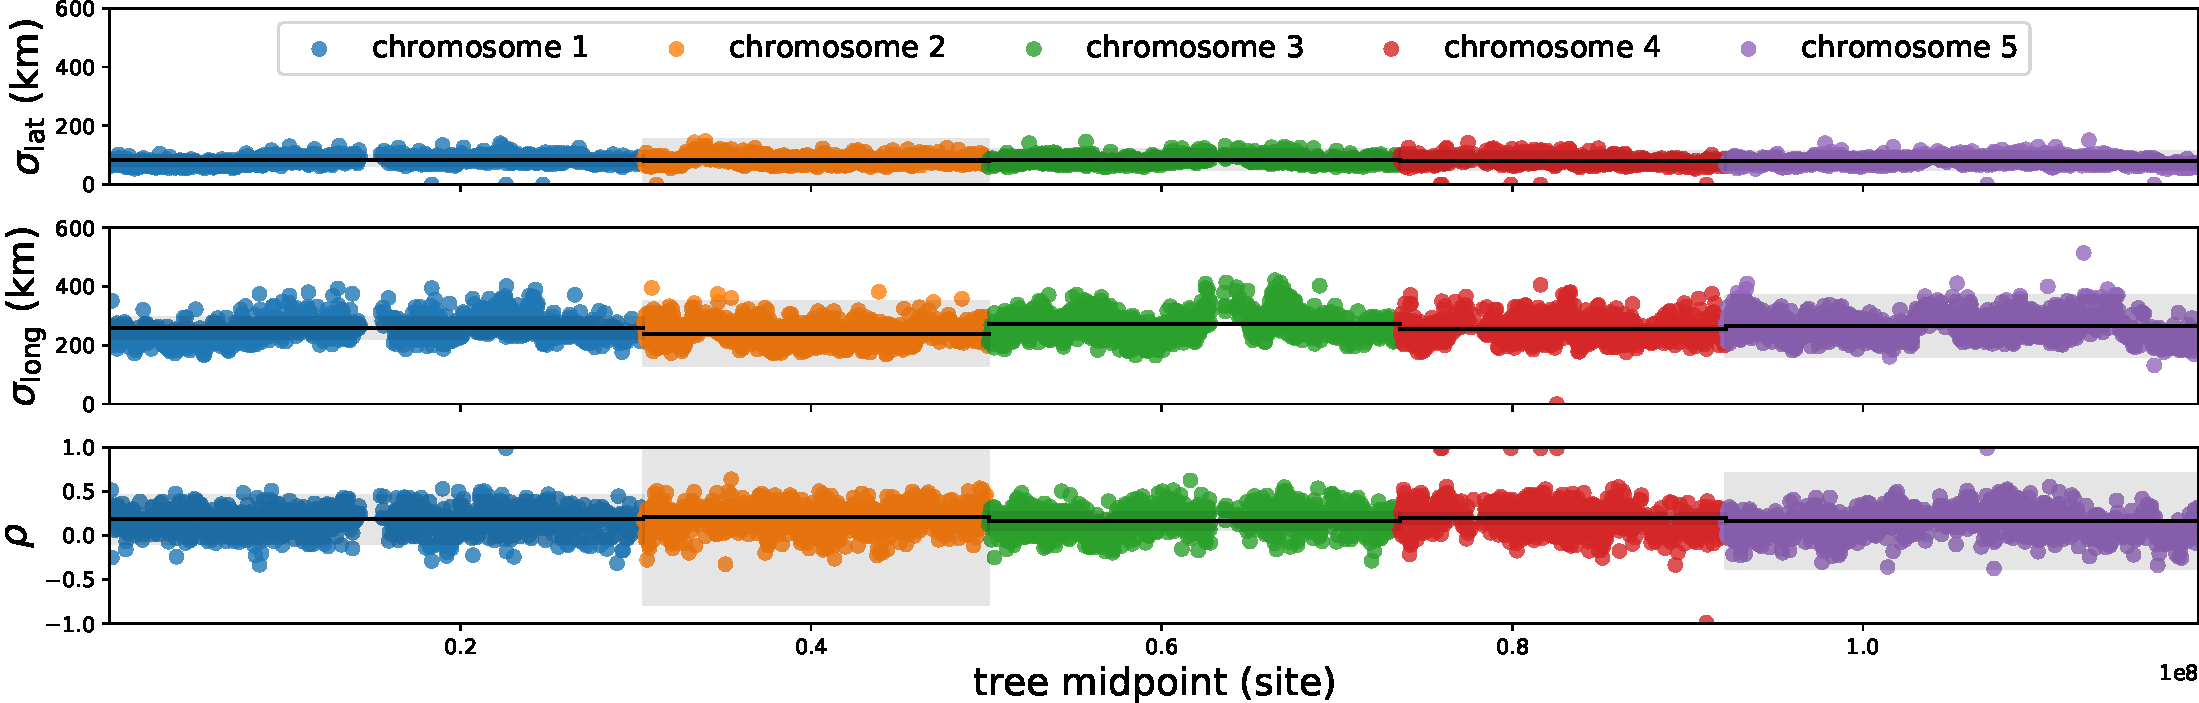
\includegraphics[width=\linewidth]{{plots/1001G_tCutoff10000_tsplits[]_groupEurasia-no-Japan_mle-dispersal.pdf}}
  };
  \node[anchor = south west] (1) at (1epoch.north west) {
    \textbf{A) One-epoch model (per-locus and per-chromosome estimates)}
  };   

  \node[below = 0.5cm of 1epoch.south west, anchor=north west] (allepoch) {
    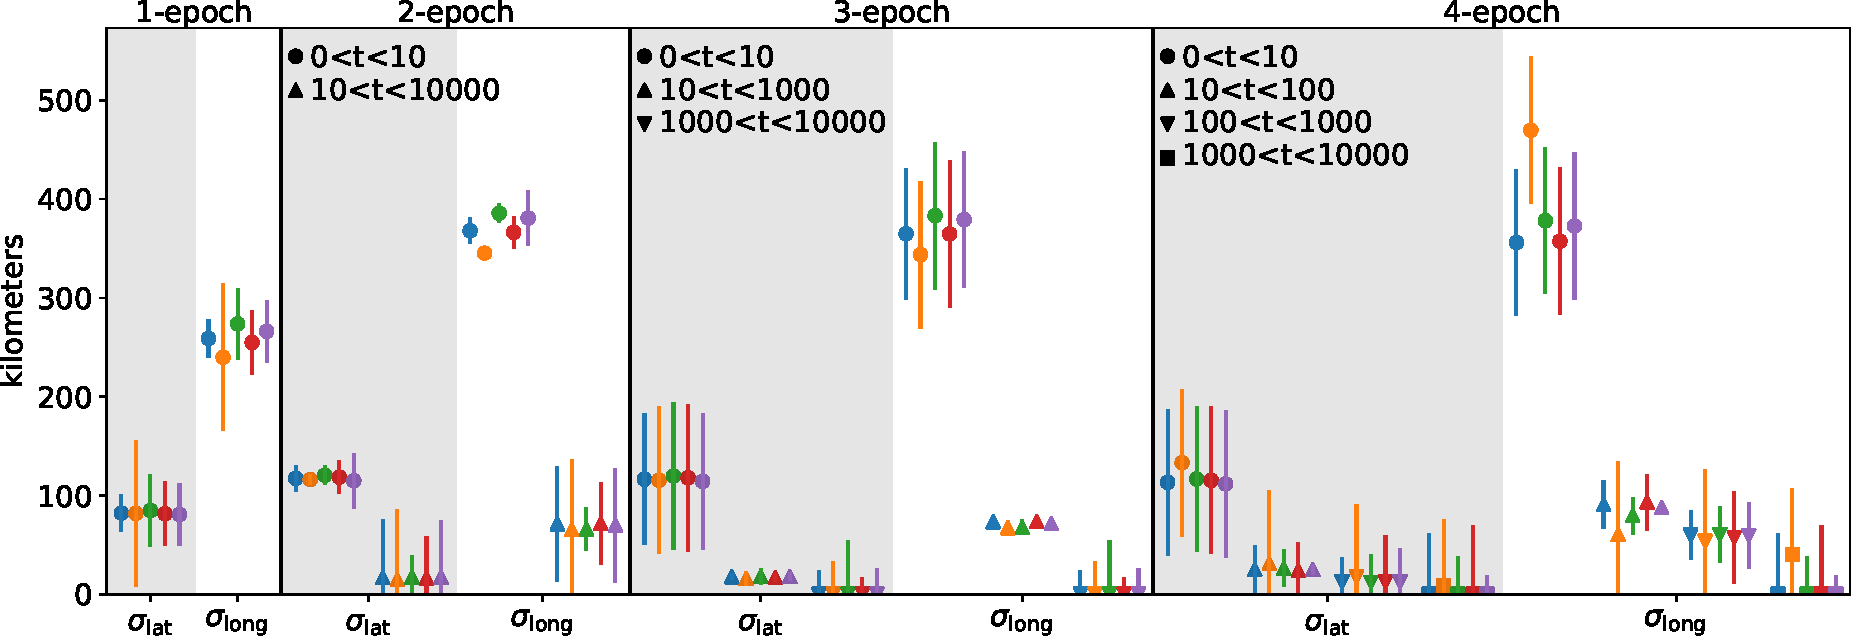
\includegraphics[width=\linewidth]{{plots/1001G_tCutoff10000_groupEurasia-no-Japan_mcle-dispersal.pdf}}
  };
  \node[anchor = south west] (3) at (allepoch.north west) {
    \textbf{B) Multi-epoch models (per-chromosome estimates only)}
  };  
  
\end{tikzpicture}  

\end{center}

\caption{
\textbf{Dispersal rate estimates in \textit{Arabidopsis thaliana}.}
\textbf{(A) One-epoch model.}
The dots are maximum likelihood estimates of dispersal rate ($\sigma$, in units of km/$\sqrt{\mathrm{generation}}$) at $10^3$ evenly-spaced loci (trees) per chromosome.
The black lines are maximum composite likelihood estimates for each chromosome (using $10^2$ evenly-spaced loci) and the grey shading is the standard error (estimated from the Hessian at the maximum). 
\textbf{(B) Multi-epoch models.}
The maximum composite likelihood dispersal rate estimates ($\pm$ standard error) across each chromosome ($10^2$ evenly-spaced loci) for models with multiple epochs (and the one-epoch model again for comparison).  
For two- and three-epoch models with alternative (and less likely) split times, see Figures \ref{fig:thal_two_epoch_dispersal} and \ref{fig:thal_three_epoch_dispersal}.
}

\label{fig:thal_sigma}
\end{figure}

%%%%%%%%%%%%%%%%%%%%%%%%%%%%%%%%%%%%%%%%%%%%%%%%%

To explore the idea that environmental changes, such as human movements and disturbance, have affected the rate of spread of \textit{A.\ thaliana}, we next estimated per-chromosome dispersal rates under a two-epoch model.
Regardless of whether the more recent epoch ends 10, $10^2$, or $10^3$ generations ago, dispersal rates in the recent epoch are greater than those under the one-epoch model (Figure \ref{fig:thal_two_epoch_dispersal}). 
Figure \ref{fig:thal_sigma}B shows the dispersal estimates under the split time with the highest likelihood (10 generations ago), suggesting very rapid dispersal along the east-west axis in very recent times (on the order of decades).
We also ran three-epoch models that allow dispersal to change at 10 and $10^2$, 10 and $10^3$, or $10^2$ and $10^3$ generations ago (Figure \ref{fig:thal_three_epoch_dispersal}). 
The model with the highest likelihood (split times of 10 and $10^3$ generations ago, Figure \ref{fig:thal_sigma}B) further supports the idea that the signal of very rapid dispersal comes from movements on the timescale of decades. 
Finally, we ran a four-epoch model with split times of 10, $10^2$, and $10^3$ generations ago (Figure \ref{fig:thal_sigma}B).
This had the highest likelihood of any model we ran and reiterates the main conclusion -- there appears to have been very rapid recent east-west dispersal. 
While it is tempting to compare dispersal rates across epochs, one caveat here is that finite habitat boundaries may disproportionally depress more ancient estimates; in essence, while we need a large recent dispersal rate to account for the large distances between relatively closely related samples, if such a dispersal rate continued far into the past the samples would be expected to cover a much wider geographic range than is possible given the constraints of habitat.

%%%%%%%%%%%%%%%%%%%%%%%%%%%%%%%%%%%%%%%%%%%%%%%%%
\subsubsection*{Identifying interesting dispersal outliers}

We next used the tree sequence and dispersal estimates to locate genetic ancestors (see \nameref{sec:methods}).
We can locate ancestors at every locus for every individual at any time, which represents an incredibly rich resource for understanding population movement.
As a first step, we visualize the mean ancestral location, averaged over loci, for every individual to detect samples with unusual geographic ancestries.
To do this we estimated the locations of recent ancestors of all samples at $100$ evenly-spaced loci per chromosome and averaged over loci to give a mean ancestral `displacement' (from the sample, backwards in time) for each sample. 

Figure \ref{fig:thal_displaced} shows these mean displacements as arrows, with colours emphasizing the length of the arrow, at 10 and $100$ generations ago.
As expected, most arrows point inwards, corresponding to the ancestors of the sample being geographically closer to one another than the samples are.
There are a few exceptions however.
For example, there is a sample in Romania (accession 9737) with a mean displacement far to the east.
This outlier appears to coalesce at many loci $\sim100$ generations ago with two samples in Russia near Kazakhstan's northeastern border (accessions 9627 and 9630), reflecting a recent long-distance dispersal event.
Taking a look at the coalescence times between accessions 9737 and 9627 along the tree sequence (Figure \ref{fig:thal_coalescence_times}A) there are many large blocks of recent coalescence ($<100$ generations), covering about $50\%$ of the genome, while the remainder of the genome coalesces more deeply.
This is consistent with the Romanian sample's previous placement in the `Asia' admixture group \citep{alonso2016}.
A second example is a sample from southern France (accession 9933) that quickly moves east to Romania/Ukraine.
Taking a look at coalescence times between this sample and those further to the east, we find this sample coalesces $<100$ generations ago with a sample from Afghanistan (accession 10015) over a few very large blocks of its genome, but is much further diverged elsewhere (Figure \ref{fig:thal_coalescence_times}B).
This is consistent with this French sample's previous `Admixed' admixture assignment \citep[including substantial ancestry from the `Central Asia' group;][]{alonso2016}. 

%%%%%%%%%%%%%%%%%%%%%%%%%%%%%%%%%%%%%%%%%%%%%%%%%
%1001g displacements%
%%%%%%%%%%%%%%%%%%%%%%%%%%%%%%%%%%%%%%%%%%%%%%%%%

\begin{figure}[!htb]

\begin{center}

\begin{tikzpicture}

  \node[text width = \linewidth] (A) {
    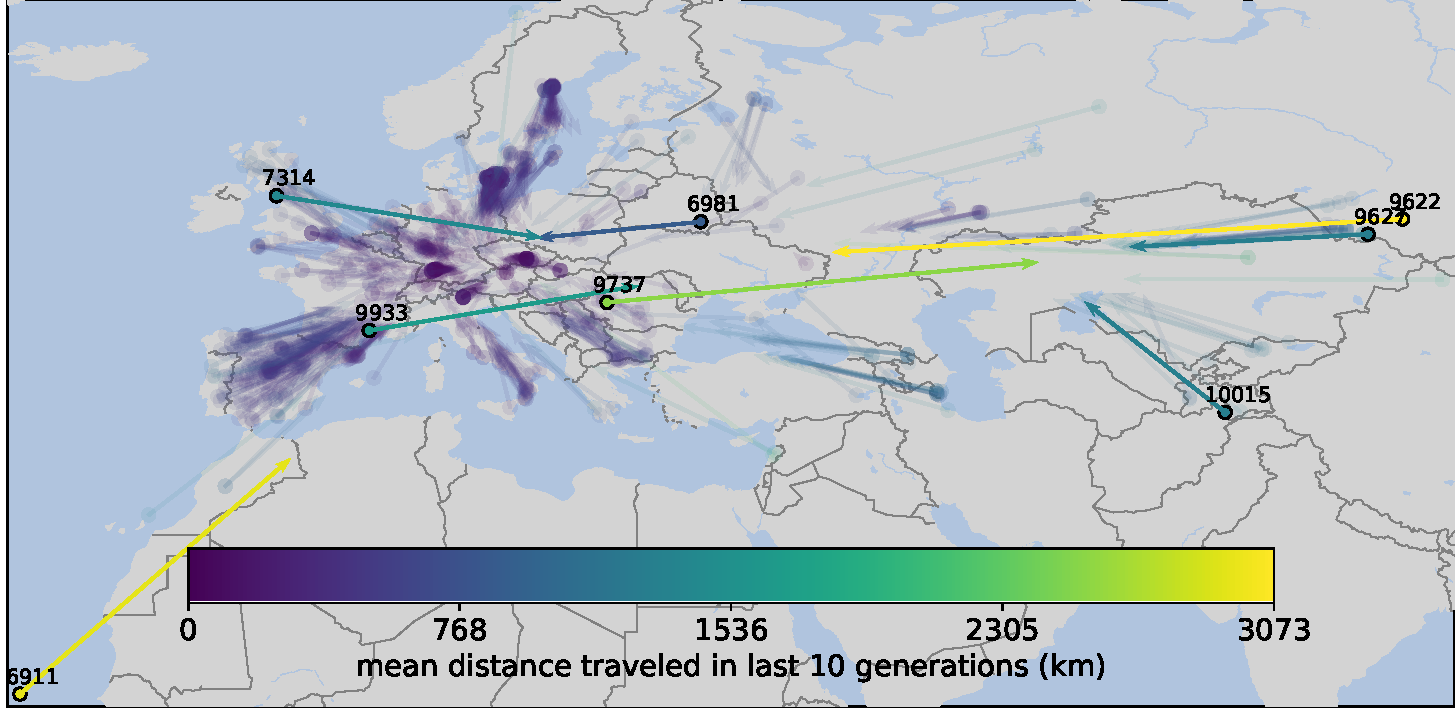
\includegraphics[width=\linewidth]{plots/1001G_mean_displacements_time10_highlights.pdf}
  };
  \node[anchor = north west, xshift = 0.5cm, yshift = -0.5cm] at (A.north west) {
    \textbf{A}
  };

 \node[text width = \linewidth, below = 0cm of A] (B) {
    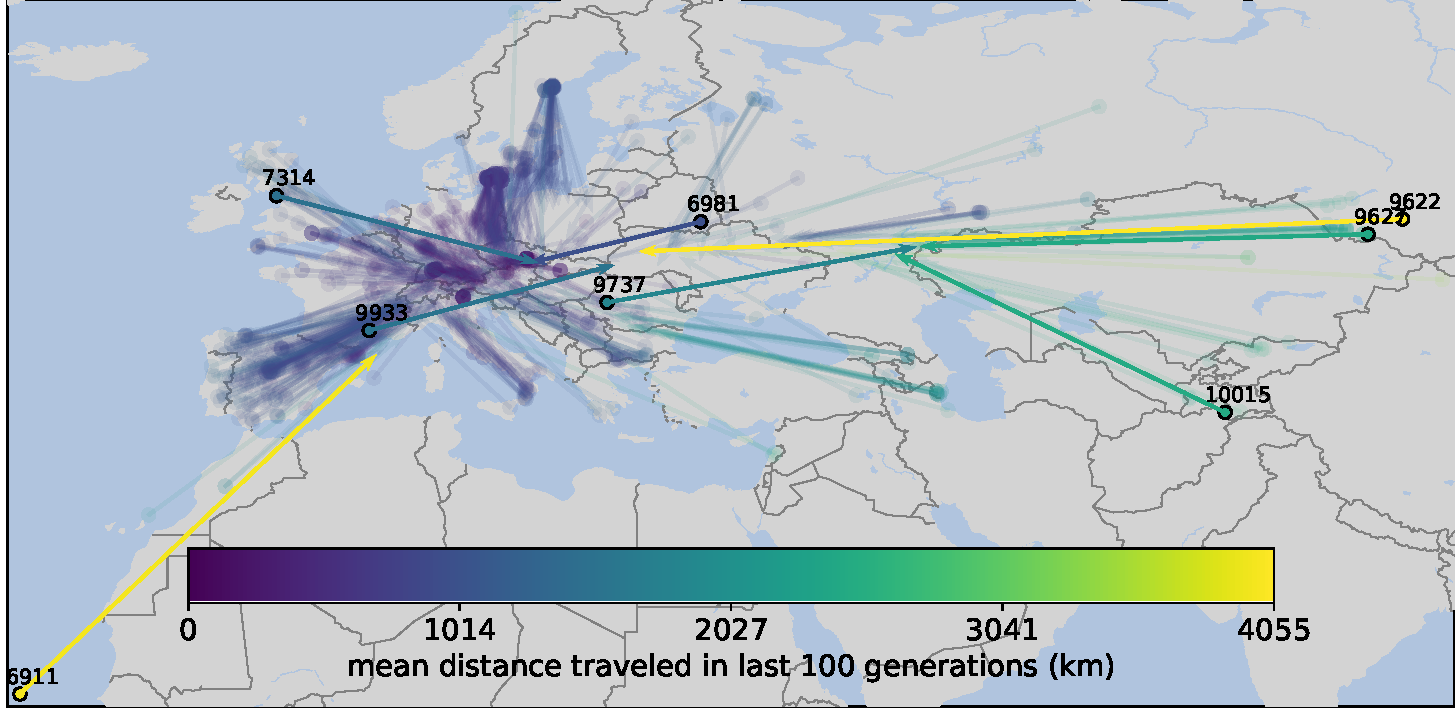
\includegraphics[width=\linewidth]{plots/1001G_mean_displacements_time100_highlights.pdf}
  };
  \node[anchor = north west, xshift = 0.5cm, yshift = -0.5cm] at (B.north west) {
    \textbf{B}
  };  
    
\end{tikzpicture}  

\end{center}

\caption{
\textbf{Locating genetic ancestors to identify interesting outliers.}
Mean maximum likelihood genetic ancestor locations (averaged over $10^2$ evenly-spaced loci per chromosome) (\textbf{A}) 10 and (\textbf{B}) $100$ generations ago.
The samples discussed in the text are highlighted and labeled (accession numbers).
Maximum likelihood locations calculated using per-chromosome four-epoch dispersal rates (Figure \ref{fig:thal_sigma}B).
}

\label{fig:thal_displaced}
\end{figure}

%%%%%%%%%%%%%%%%%%%%%%%%%%%%%%%%%%%%%%%%%%%%%%%%%

There are also some samples that are outliers in terms of distance traveled by their ancestors.
For example, there are two samples, one from the UK (accession 7314) and the other from Belarus (accession 6981), that travel long distances towards one another in the past $\sim10$ generations (see also Figure 3B in \citep{alonso2016}). 
A look at the coalescence times between these two samples shows that these two individuals are extremely closely related along almost all of their genome except the first $\approx700$kb of chromosome 5 (Figure \ref{fig:thal_coalescence_times}C).
Other outliers include the sample from Cabo Verde (accession 6911), which is classified as a Relict but includes a large amount of European ancestry \citep{alonso2016} and the most eastward Russian sample (accession 9622), which has substantial European ancestry \citep{alonso2016}.
More generally, we also see greater rates of movement, on average, from samples from further east, consistent with the previous finding of reduced genetic distance between `Asian' samples up to $\sim$250km apart \citep{alonso2016}, the signal of a rapid eastward expansion. 

%%%%%%%%%%%%%%%%%%%%%%%%%%%%%%%%%%%%%%%%%%%%%%%%%
\subsubsection*{Detecting the existence and source of rare long-distant migrants and misplaced samples}

We next looked in more detail at some of the largest outliers in recent ancestral movements.
As mentioned above, the two accessions from Japan are thought to be recent long-distance migrants.
When we include these samples' locations and locate their ancestors, these samples are the largest outliers in their inferred rate of recent movement (result not shown).
Creating a smooth kernel from $10^3$ inferred ancestral locations per chromosome, Figure \ref{fig:thal_outliers}A shows an extremely rapid transition between Japan and Europe in the last $\sim10-100$ generations (only accession 7207 shown).
This is consistent with the hypothesis that humans moved the ancestors of these samples from Europe to Japan in the last few hundred years \citep{zou2017adaptation}. 

%%%%%%%%%%%%%%%%%%%%%%%%%%%%%%%%%%%%%%%%%%%%%%%%%
%long-distant dispersal and misplaced samples%
%%%%%%%%%%%%%%%%%%%%%%%%%%%%%%%%%%%%%%%%%%%%%%%%%

\begin{figure}[!b]

\begin{center}

\begin{tikzpicture}

  % long distance dispersal
  \node[] (jpn_time1) {
    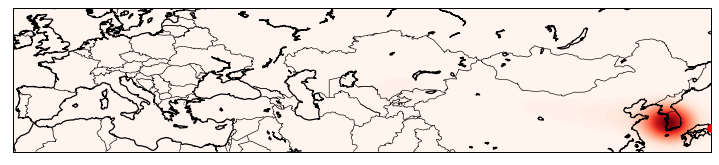
\includegraphics[width=\linewidth]{plots/1001G_ancestor-location-density-map_node431_time1_tsplits[10,100,1000].png} 
  };
  \node[below = -0.25cm of jpn_time1] (jpn_time2) {
    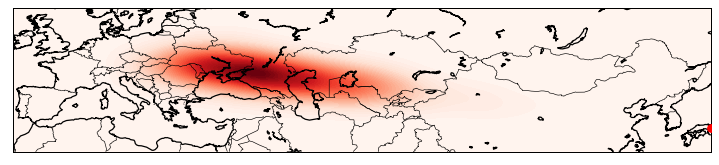
\includegraphics[width=\linewidth]{plots/1001G_ancestor-location-density-map_node431_time10_tsplits[10,100,1000].png} 
  };
  \node[below = -0.25cm of jpn_time2] (jpn_time3) {
    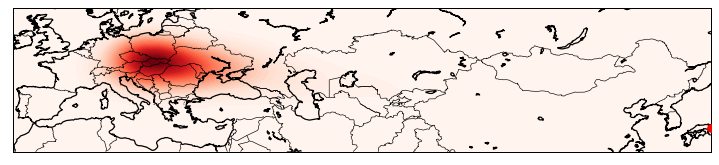
\includegraphics[width=\linewidth]{plots/1001G_ancestor-location-density-map_node431_time100_tsplits[10,100,1000].png} 
  };
  \node[left = 0cm of jpn_time1, rotate = 90, anchor=center, ] {\small 1 years ago};
  \node[left = 0cm of jpn_time2, rotate = 90, anchor=center] {\small 10 years ago};
  \node[left = 0cm of jpn_time3, rotate = 90, anchor=center] {\small $100$ years ago};
  \node[above = 0cm of jpn_time1.north west, anchor= west, color = red, xshift=0.25cm] {\textbf{A} Long-distance dispersal \scriptsize(accession 7207)};
  
  % misplaced sample
  \node[below = 0.25cm of jpn_time3.south west, anchor = north west] (misplaced_time1) {
    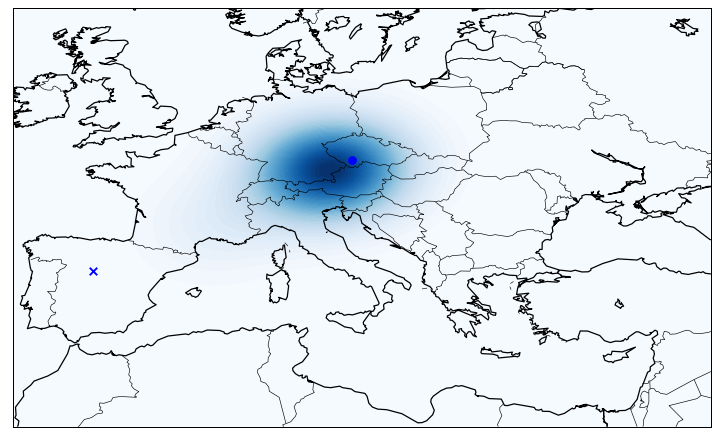
\includegraphics[width=0.5\linewidth]{plots/1001G_misplaced-ancestor-location-density-map_node697_time1_tsplits[10,100,1000].png}
  };
  \node[right = -0.25cm of misplaced_time1] (misplaced_time2) {
    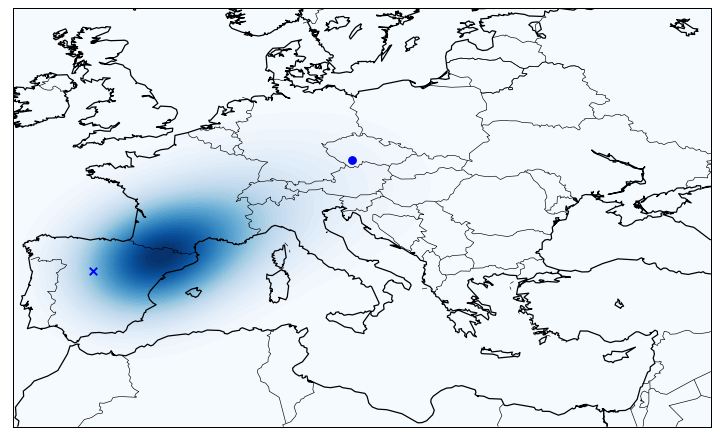
\includegraphics[width=0.5\linewidth]{plots/1001G_misplaced-ancestor-location-density-map_node697_time10_tsplits[10,100,1000].png}
  };
  \node[left = 0cm of misplaced_time1, rotate = 90, anchor=center] {\small 1 years ago};
  \node[right = 0cm of misplaced_time2, rotate = 270, anchor=center] {\small 10 years ago};
  \node[above = 0cm of misplaced_time1.north west, anchor= west, color = blue, xshift=0.25cm] {\textbf{B} Misplaced sample \scriptsize(accession 9533)};

\end{tikzpicture}  
\end{center}
\caption{(Continued on the following page.)}
\label{fig:thal_outliers}
\end{figure}

\begin{figure}[!t]
\contcaption{
\textbf{Locating genetic ancestors to detect the existence and source of (A) recent long-distance dispersal and (B) misplaced samples}.
Shown are density kernels of the maximum likelihood ancestral locations at $10^3$ evenly-spaced loci per chromosome for (\textbf{A}) a Japanese accession (100\% `Central Europe' ancestry) and (\textbf{B}) an Iberian Relict (100\% Relict ancestry) from Spain that we misplaced to the mean location of all samples (Czech Republic).
The dots show the assumed sample locations (at the edge of the panes in \textbf{A}) and the `x' in \textbf{B} shows the true sample location.
Maximum likelihood locations calculated using per-chromosome four-epoch dispersal rates (Figure \ref{fig:thal_sigma}B).
}
\end{figure}
%%%%%%%%%%%%%%%%%%%%%%%%%%%%%%%%%%%%%%%%%%%%%%%%%

The Japanese samples, while spatial outliers, are relatively closely related to the majority of the other samples \citep{alonso2016}. 
Thus, our method has the power to locate their ancestors and detect them as recent migrants.
To see if the our method, and the data, have the power to detect a recent migrant from a less well represented ancestry, we deliberately misplaced the location of an Iberian Relict from Spain (accession 9533) to the mean location of the Eurasian samples after filtering (southern Czech Republic).
Since this is an Iberian Relict, it is most closely related to the 21 other Iberian Relict samples (only $\approx2\%$ of the samples), with much of its ancestry likely coming from a refuge in north Africa \citep{alonso2016,durvasula2017african,fulgione2018madeiran}.
Figure \ref{fig:thal_outliers}B shows that, despite the rarity of this ancestry in this dataset, our method correctly puts the misplaced Relict back into Spain at most loci in $\sim10$ generations.

The examples above show that our method has the power to detect many recent long-distant migrants and misplaced samples, and identify their source.
Note that, because we assume a model of continuous migration, the ancestors of recent migrants and misplaced samples have to migrate through intermediate locations to reach their likely source location. 
However, if, after inspection, an investigator suspects that a sample was likely misplaced, or dispersed a long distance suddenly, they could choose to ignore that sample's location and use the trees alone to estimate its source. 

%%%%%%%%%%%%%%%%%%%%%%%%%%%%%%%%%%%%%%%%%%%%%%%%%
\subsubsection*{Inferring the origin and ancestry of a recent invasion}

To illustrate how we can use our method to identify the source location of a subset of samples (e.g., recent migrants or misplaced samples), we used our method to infer the origin and ancestry of the 125 accessions from the recent expansion of \textit{A. thaliana} into North America.
We did this by ignoring the locations of these samples and predicting their current and ancestral locations based only on the trees and the locations of the remaining samples. 
Figure \ref{fig:thal_NA} shows the predicted current (purple) and ancestral locations, averaged over $10^2$ loci per chromosome, for each North American accession.
This does two things. 
First, if we knew the time of colonization, we could read off where we expect the colonization to have originated from.
Instead of simply asking where are the most closely related samples, we allow all the lineages to move backwards in time, naturally correcting for the movement of lineages between the time of sampling and the time of colonization.
In this case, the colonization of North America by \textit{A. thaliana} is thought to be about 400 years ago \citep{exposito2018rate}, suggesting that the majority of the North American accessions came from southern Germany, despite being more closely related, in many cases, to samples in north eastern France today.
Second, Figure \ref{fig:thal_NA} helps visualize the high degree of relatedness among the North American samples. 
For instance, a large group of closely related North American samples are also closely related to current-day samples in north eastern France, and appear to coalesce with one another at many loci in the last few hundred years, near the purported time of colonization.
On the other hand, there is a handful of more distantly related North American samples, most closely related to present-day samples ranging from northern Germany to Russia, that do not coalesce at most loci in the past $10^3$ years, suggesting multiple colonizations of North America, as previously hypothesized \citep{exposito2018rate}.
Encouragingly, connecting the sample and inferred locations (Figure \ref{fig:thal_NA_connected}), we find that the samples placed in Russia and Slovakia are from near Manistee, Michigan (accessions 1890 and 2202) and the sample placed near northern Germany is the reference, Col-0, from Missouri (accession 6909), consistent with recent independent findings \citep{shirsekar2021fine}.

%%%%%%%%%%%%%%%%%%%%%%%%%%%%%%%%%%%%%%%%%%%%%%%%%
%1001g locating NAs figure%
%%%%%%%%%%%%%%%%%%%%%%%%%%%%%%%%%%%%%%%%%%%%%%%%%

\begin{figure}[!b]
\begin{center}
\begin{tikzpicture}

  \node[] (time1000) {
    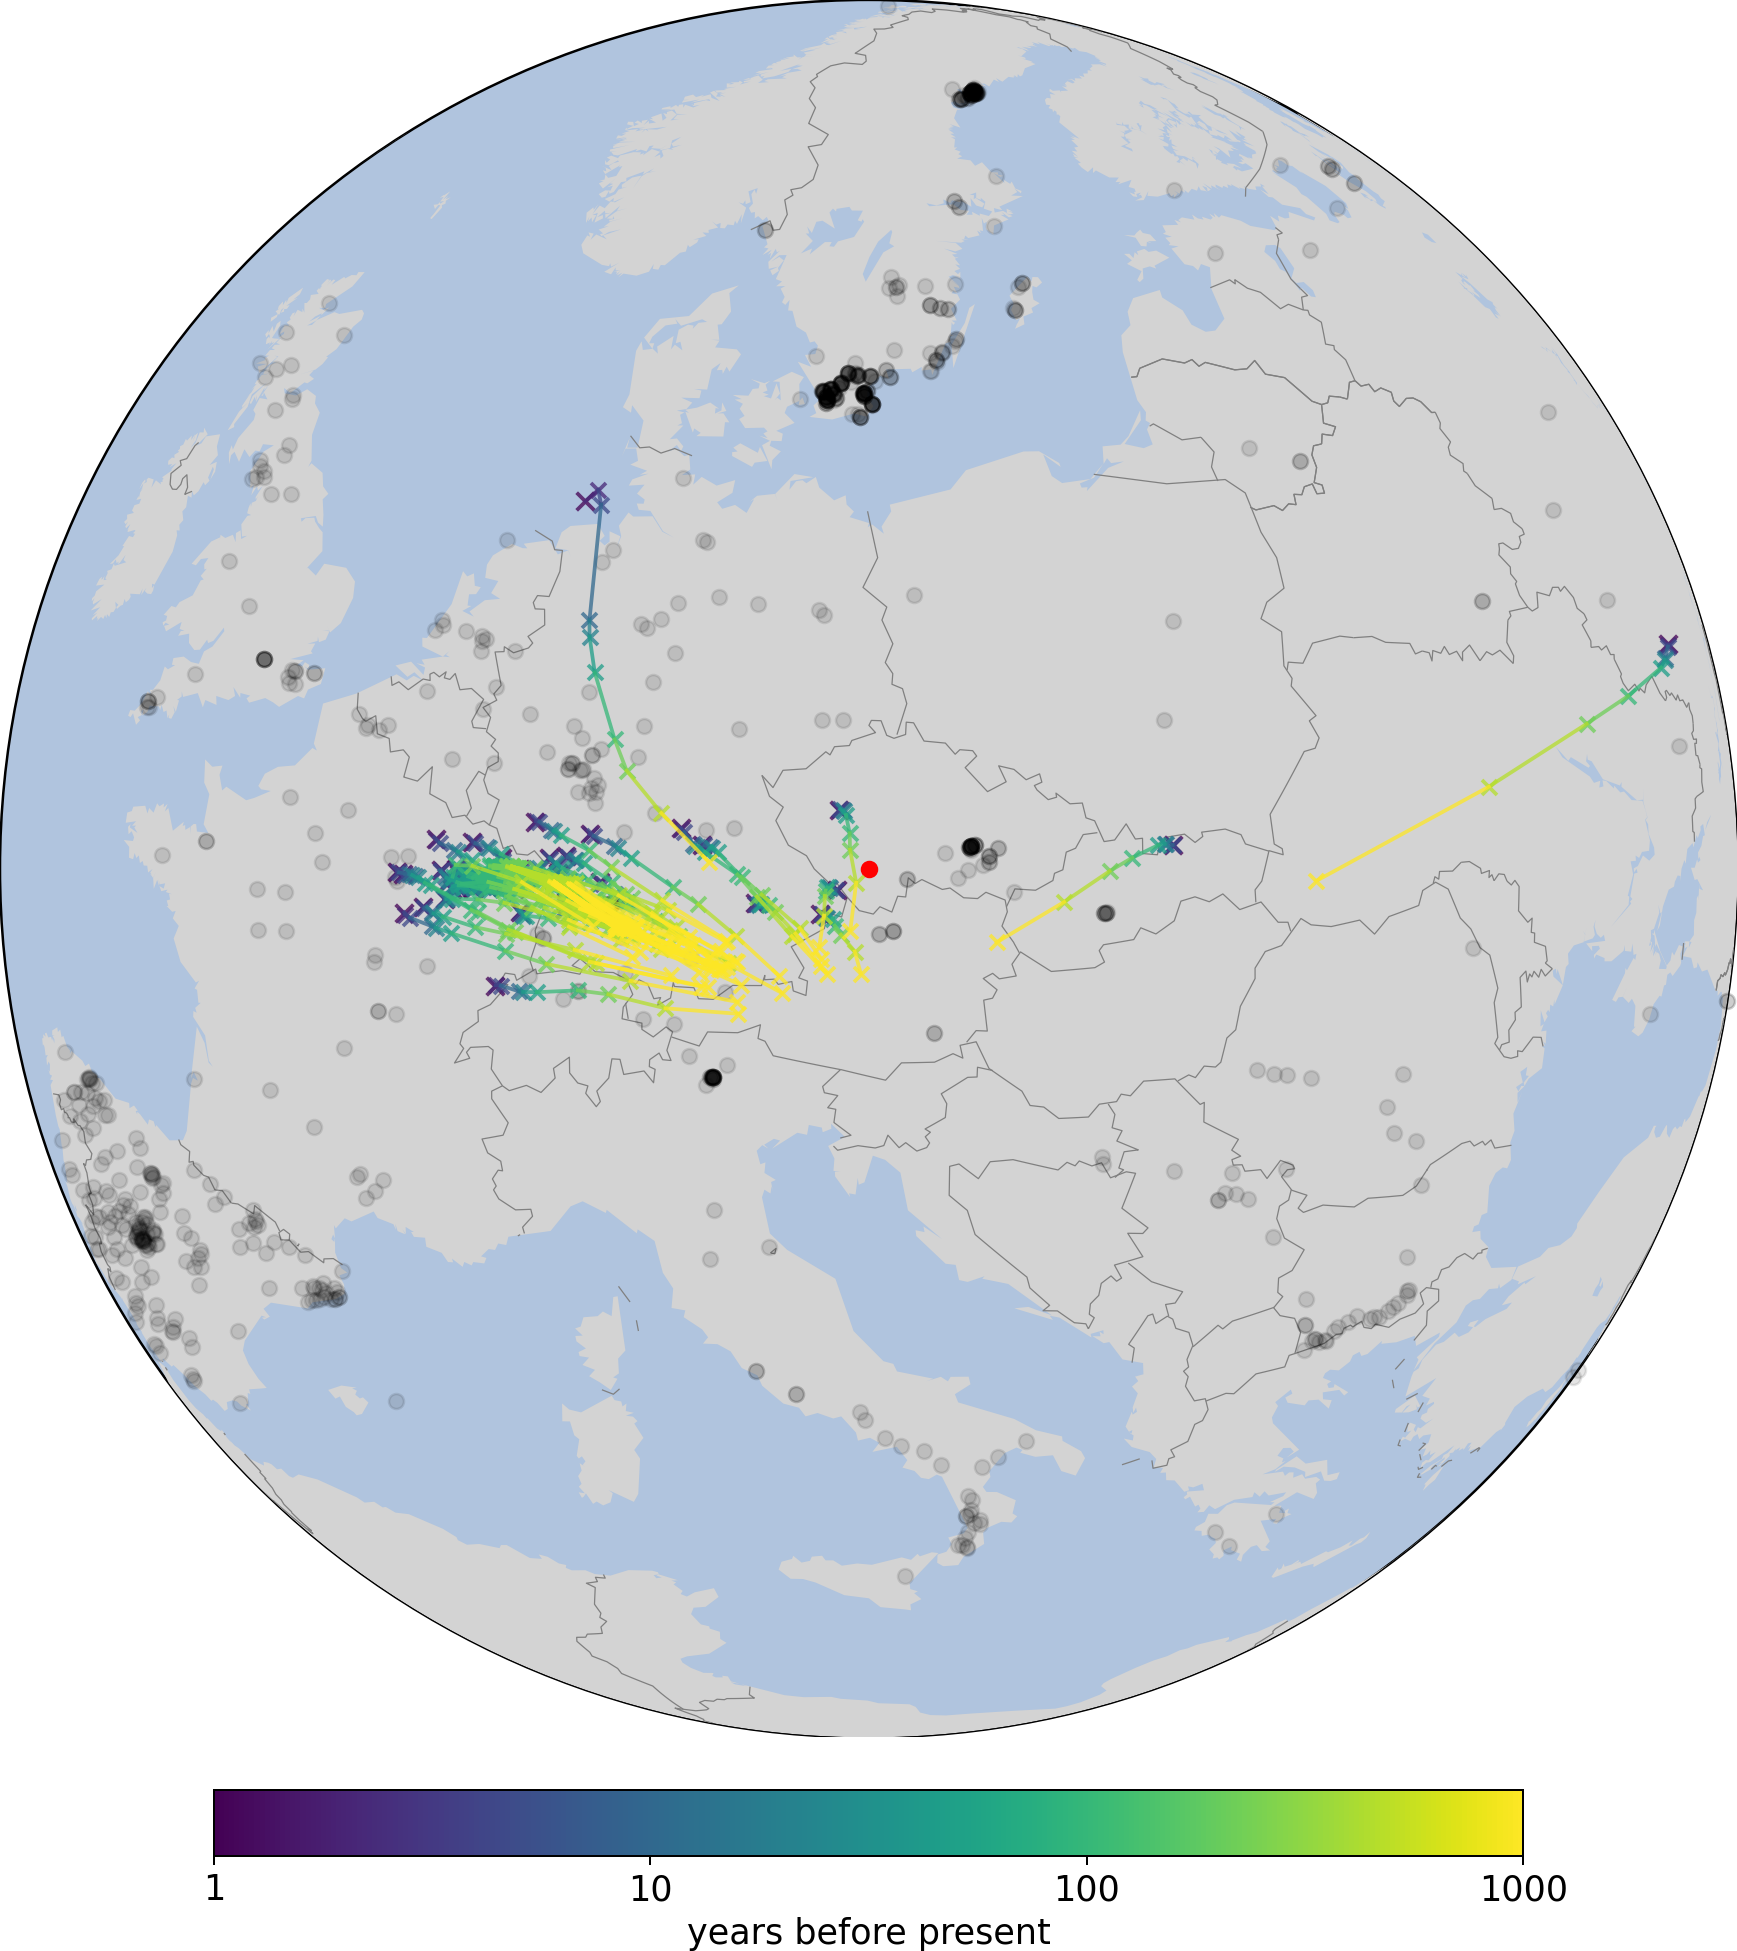
\includegraphics[width=1\linewidth]{1001G_NA-locations_tsplits[10,100,1000].png}
  };
  
\end{tikzpicture}  
\end{center}
\caption{(Continued on the following page.)}
\label{fig:thal_NA}
\end{figure}
\begin{figure}[!t]
\contcaption{
\textbf{Locating genetic ancestors to identify the source and ancestry of recent expansions/colonizations.}
Mean maximum likelihood genetic ancestor locations (averaged over $10^2$ evenly-spaced loci per chromosome) of the 125 North American accessions over the last $10^3$ years.
The black dots are sample locations and the red dot is their mean.
Maximum likelihood locations calculated using per-chromosome four-epoch dispersal rates (Figure \ref{fig:thal_sigma}B).
}
\end{figure}

%%%%%%%%%%%%%%%%%%%%%%%%%%%%%%%%%%%%%%%%%%%%%%%%%

%%%%%%%%%%%%%%%%%%%%%%%%%%%%%%%%%%%%%%%%%%%%%%%%%
\subsubsection*{Visualizing alternative geographic ancestries}

As mentioned above, the 1001 Genomes dataset is thought to contain samples drawing ancestors from at least two different glacial refugia, including the Non-Relict samples with ancestry predominately from a Balkan refuge \citep{lee2017post} and the Iberian Relict samples with substantial ancestry from a refuge in north Africa \citep{alonso2016,durvasula2017african,fulgione2018madeiran}.
We therefore sought to use our method to visualize these alternative geographic ancestries.

We first compared the geographic ancestries of three representative accessions from Spain (Figure \ref{fig:thal_ancestries}): one from a Non-Relict admixture group (accession 6933; 100\% `Spain' ancestry); one from the Relict admixture group (accession 9533; 100\% Relict ancestry); and one drawing roughly equal ancestry from both these groups (accession 9530; 57\% Relict and 43\% `Spain' ancestry).
As expected given the glacial refuge of the Non-Relict lineages is thought to be near the Balkans \citep{lee2017post}, the Non-Relict sample's genetic ancestors move gradually and coherently north east, out of the Iberian Peninsula by 200 years ago and into northern Italy/Austria by 500 years ago. 
In contrast, a large proportion of the Relict sample's ancestors remain on the Iberian Peninsula for the last 500 years, where the rest of the closely related Iberian Relict samples are clustered.
The Admixed sample's genetic ancestors display much more variability, with the rate of return to the east depending on the ancestry at each locus, with many ancestors still remaining in Spain but many already in Italy $\approx200$ years ago. 

%%%%%%%%%%%%%%%%%%%%%%%%%%%%%%%%%%%%%%%%%%%%%%%%%
%Non-Relict - Admixed  - Relict%
%%%%%%%%%%%%%%%%%%%%%%%%%%%%%%%%%%%%%%%%%%%%%%%%%

\begin{figure}[!htb]

\begin{center}

\begin{tikzpicture}

  % plots
  \node[] (time1) {
    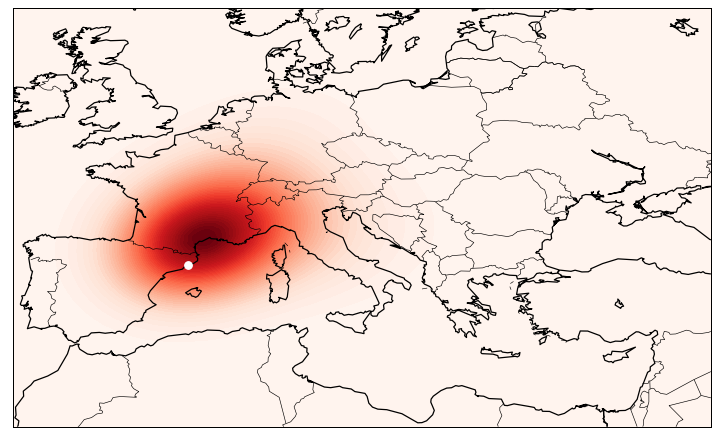
\includegraphics[width=0.33\linewidth]{plots/1001G_ancestor-location-density-map_node338_time10_tsplits[10,100,1000].png}
    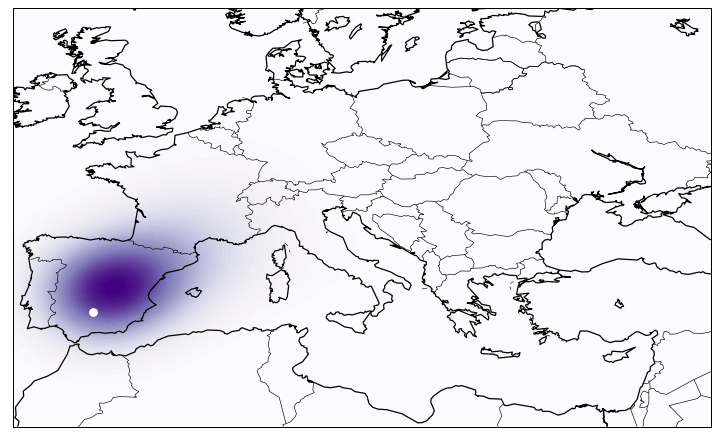
\includegraphics[width=0.33\linewidth]{plots/1001G_ancestor-location-density-map_node694_time10_tsplits[10,100,1000].png}
    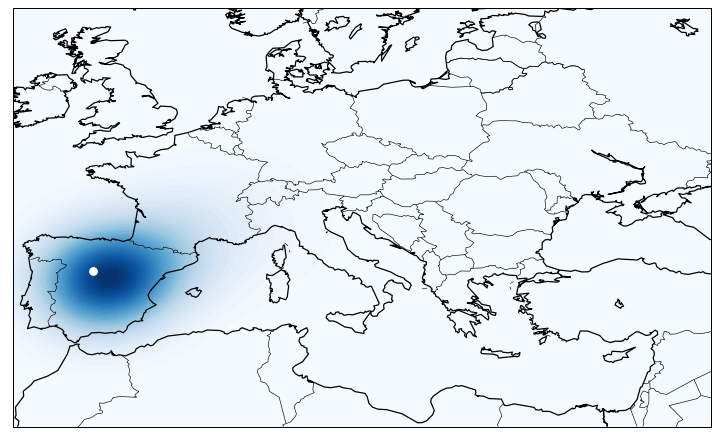
\includegraphics[width=0.33\linewidth]{plots/1001G_ancestor-location-density-map_node697_time10_tsplits[10,100,1000].png}
  };
  \node[below = -0.25cm of time1] (time2) {
    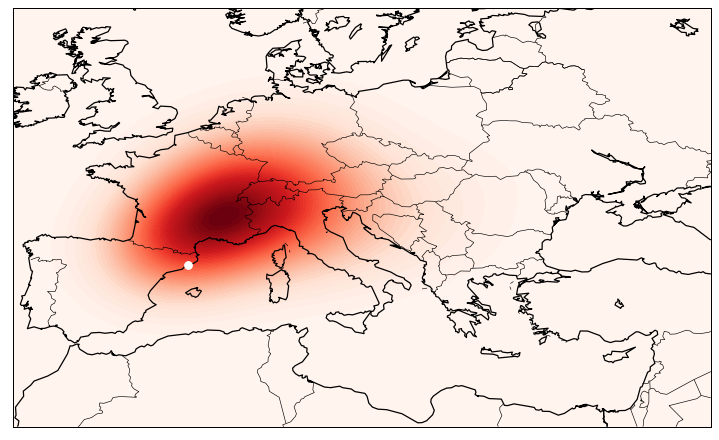
\includegraphics[width=0.33\linewidth]{plots/1001G_ancestor-location-density-map_node338_time100_tsplits[10,100,1000].png}
    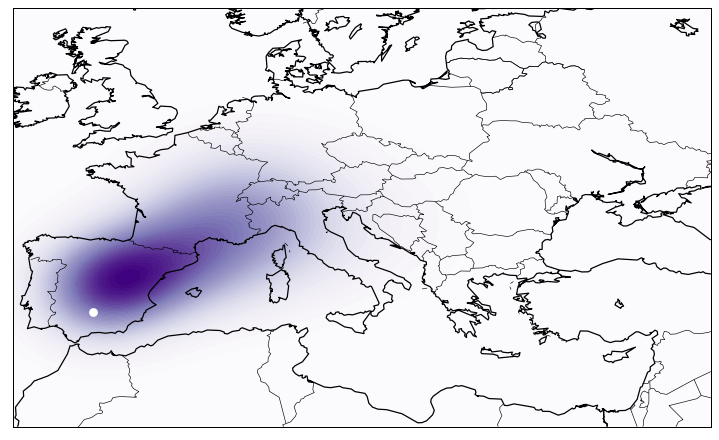
\includegraphics[width=0.33\linewidth]{plots/1001G_ancestor-location-density-map_node694_time100_tsplits[10,100,1000].png}
    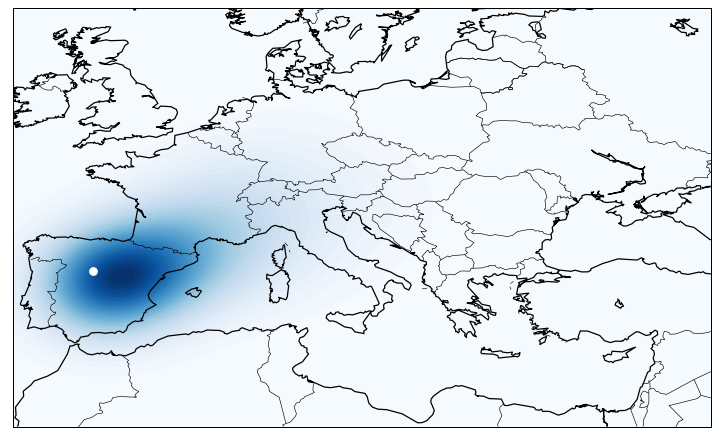
\includegraphics[width=0.33\linewidth]{plots/1001G_ancestor-location-density-map_node697_time100_tsplits[10,100,1000].png}
  };
  \node[below = -0.25cm of time2] (time3) {
    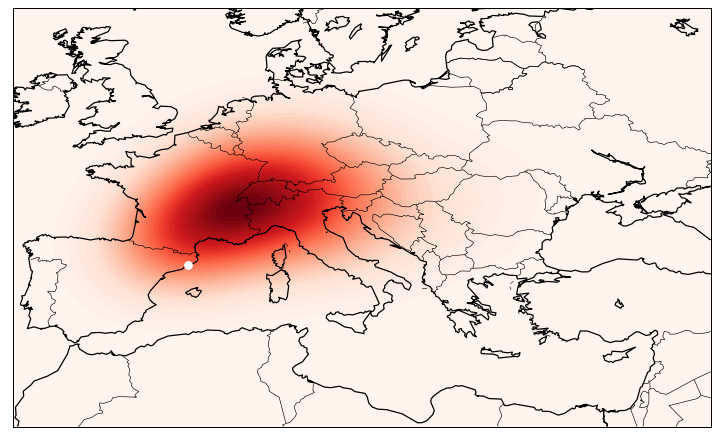
\includegraphics[width=0.33\linewidth]{plots/1001G_ancestor-location-density-map_node338_time215_tsplits[10,100,1000].png}
    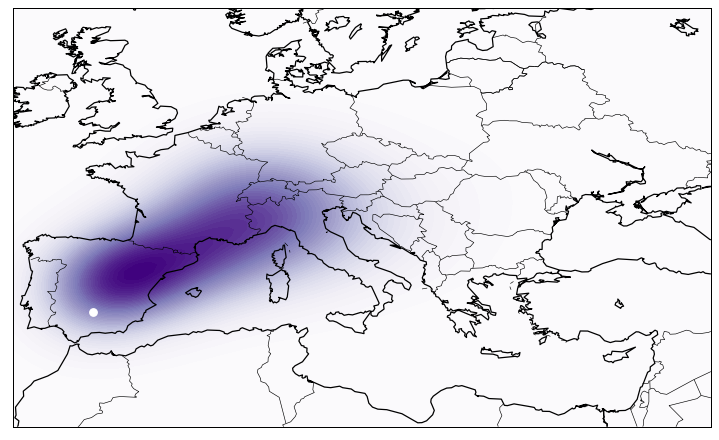
\includegraphics[width=0.33\linewidth]{plots/1001G_ancestor-location-density-map_node694_time215_tsplits[10,100,1000].png}
    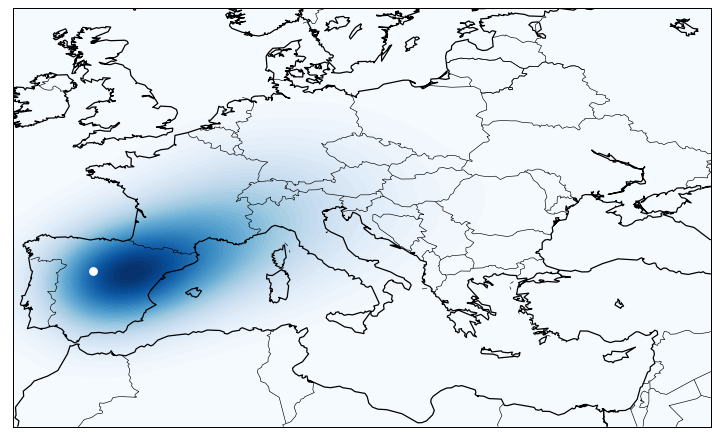
\includegraphics[width=0.33\linewidth]{plots/1001G_ancestor-location-density-map_node697_time215_tsplits[10,100,1000].png}
  };
  \node[below = -0.25cm of time3] (time4) {
    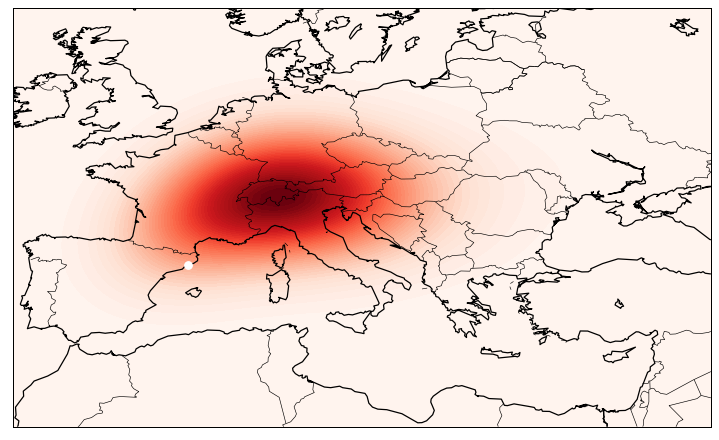
\includegraphics[width=0.33\linewidth]{plots/1001G_ancestor-location-density-map_node338_time464_tsplits[10,100,1000].png}
    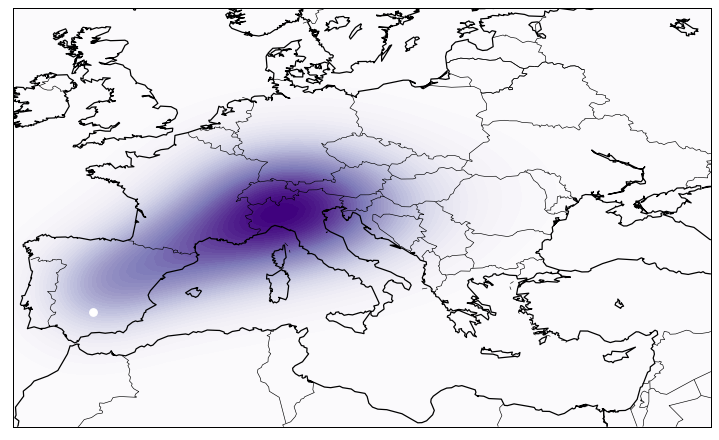
\includegraphics[width=0.33\linewidth]{plots/1001G_ancestor-location-density-map_node694_time464_tsplits[10,100,1000].png}
    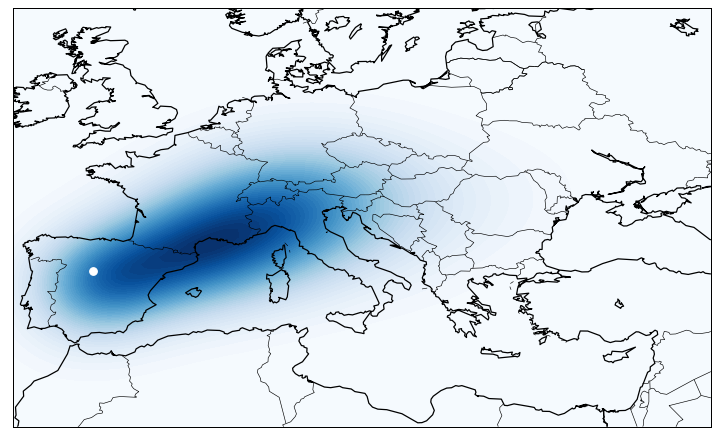
\includegraphics[width=0.33\linewidth]{plots/1001G_ancestor-location-density-map_node697_time464_tsplits[10,100,1000].png}
  };

  % column labels
  \node[above = 0cm of time1.north west, anchor = west, color = red] {Non-Relict \scriptsize(accession 6933)};
  \node[above = 0cm of time1.north west, anchor = west, color = red!50!blue, xshift = 0.34\linewidth] {Admixed \scriptsize(accession 9530)};
  \node[above = 0cm of time1.north west, anchor = west, color = blue, xshift = 0.68\linewidth] {Relict \scriptsize(accession 9533)};

  % row labels
  \node[left = 0cm of time1, rotate = 90, anchor=center, ] {\small 10 years ago};
  \node[left = 0cm of time2, rotate = 90, anchor=center] {\small 100 years ago};
  \node[left = 0cm of time3, rotate = 90, anchor=center] {\small 215 years ago};
  \node[left = 0cm of time4, rotate = 90, anchor=center] {\small 464 years ago};
  
\end{tikzpicture}  

\end{center}

\caption{
\textbf{Locating genetic ancestors to depict alternative geographic histories}.
Genetic ancestors of three samples from Spain from three different admixture groups: a Non-Relict (100\% `Spain'), an Admixed (43\% `Spain', 57\% Relict), and an Iberian Relict (100\% Relict).
Shown are density kernels of the maximum likelihood ancestral locations using $10^3$ evenly-spaced loci per chromosome.
White dots show the sample locations.
Maximum likelihood locations calculated using per-chromosome four-epoch dispersal rates (Figure \ref{fig:thal_sigma}B).
}

\label{fig:thal_ancestries}
\end{figure}
%%%%%%%%%%%%%%%%%%%%%%%%%%%%%%%%%%%%%%%%%%%%%%%%%

To confirm this is a general pattern beyond these three representative samples, we also looked at the mean ancestral displacements (over $10^2$ loci per chromosome) of all mainland Spanish samples from each of the three groups (Relict, Non-Relict, and Admixed; Figure \ref{fig:thal_spanish_moves}).
We see that, on average, Non-Relict samples tend to move both further north and further east than the Relict samples, in the direction of the mean sample location and towards the Balkans (the same conclusions are reached if we compare just the `Spain' and Relict groups, results not shown).
The Admixed  samples show much more variation in the amount of northward displacement, as expected given these samples could have ancestries from any two or more groups, including two Non-Relict groups (e.g., `Spain' and `North Sweden').

%%%%%%%%%%%%%%%%%%%%%%%%%%%%%%%%%%%%%%%%%%%%%%%%%
%1001g spanish displacements%
%%%%%%%%%%%%%%%%%%%%%%%%%%%%%%%%%%%%%%%%%%%%%%%%%

\begin{figure}[!htb]
\begin{center}

\begin{tikzpicture}
  
  \node[] (A) {  
    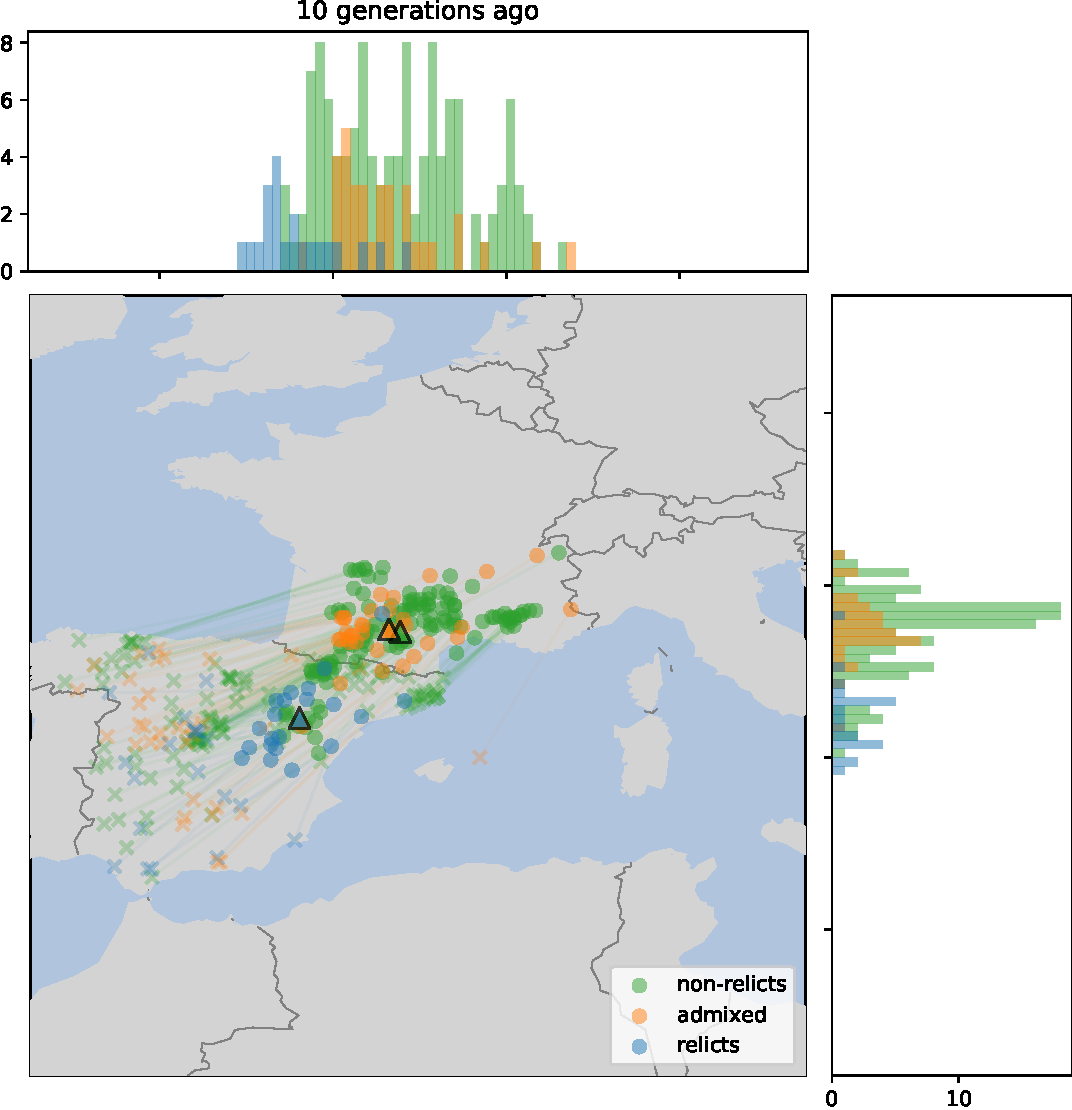
\includegraphics[width=0.5\linewidth]{{plots/1001G_spanish-moves_time10.pdf}}
  };
  \node[anchor = north east] at ($(A.north east) + (-0.75, -0.75)$) {
    \textbf{A}
  };


  \node[right = 0cm of A] (B) {  
    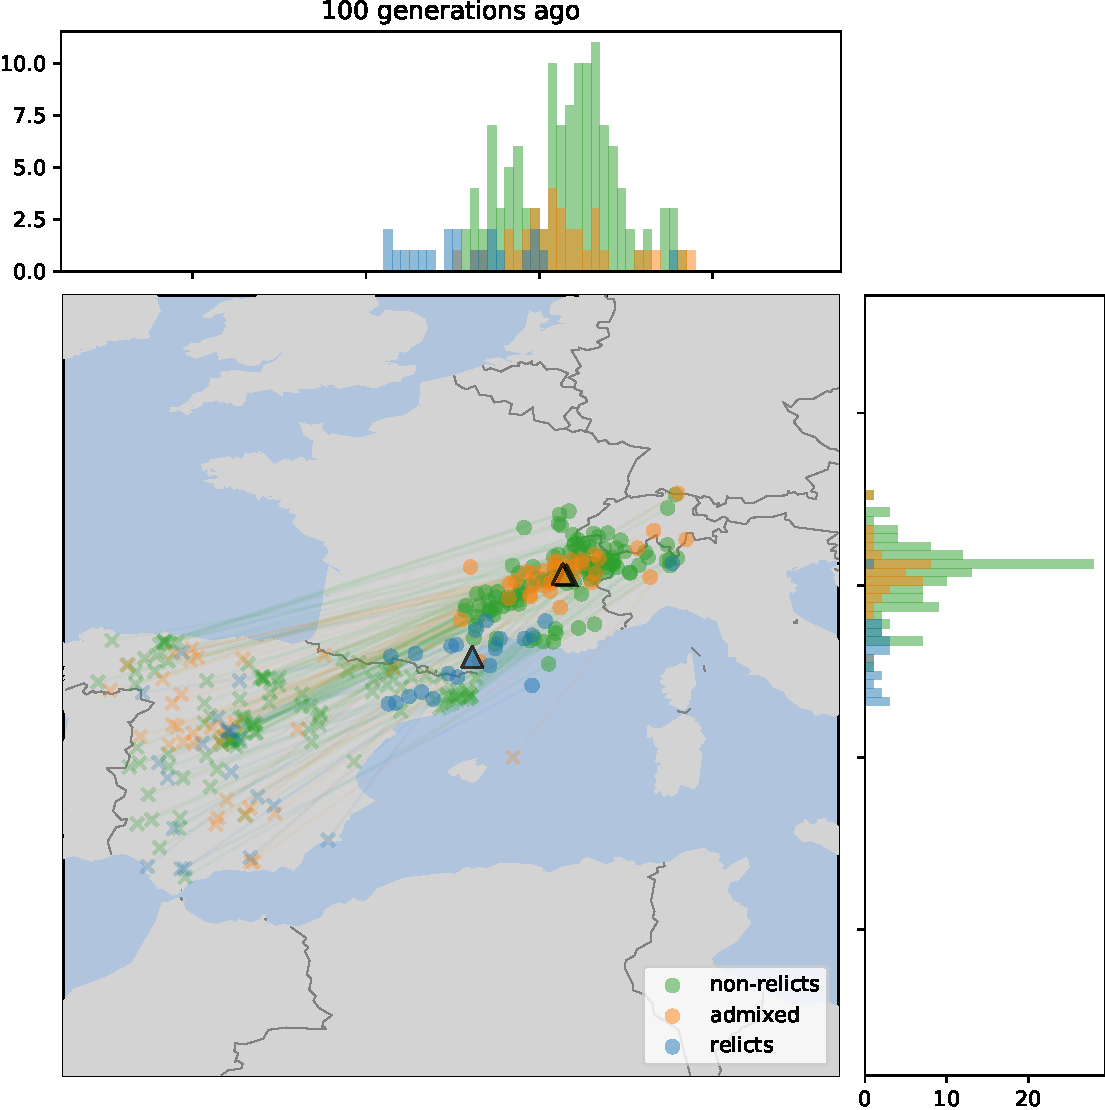
\includegraphics[width=0.5\linewidth]{{plots/1001G_spanish-moves_time100.pdf}}
  };
  \node[anchor = north east] at ($(B.north east) + (-0.75, -0.75)$) {
    \textbf{B}
  };


\end{tikzpicture}

\end{center}

\caption{
\textbf{Relict samples display an alternative geographic history.}
Mean genetic ancestor locations of all samples from Spain (excluding the Canary Islands) by admixture group.
Data as in Figure \ref{fig:thal_displaced}, with `x's the sample locations and `o's the mean ancestor location and lines connecting them.
Colours indicate admixture group (Non-Relict is any group besides Relict or Admixed; Admixed is any sample with $<60\%$ ancestry in all groups \citep{alonso2016}).
Triangles indicate mean locations for each admixture group.
Maximum likelihood locations calculated using per-chromosome four-epoch dispersal rates (Figure \ref{fig:thal_sigma}B).
}
\label{fig:thal_spanish_moves}
\end{figure}

%%%%%%%%%%%%%%%%%%%%%%%%%%%%%%%%%%%%%%%%%%%%%%%%%%%%%%%

Eventually nearly all of an Iberian Relict sample's ancestors are pulled east, perhaps because the Iberian Relict ancestry is only represented by $\sim2\%$ of the samples, but perhaps also because the Iberian Relicts are through to have extensive admixture with the Non-Relicts  \citep{fulgione2018madeiran}.
There are only three samples from Africa in the 1001 Genomes dataset (accessions 6911, 9606, and 9939), all of which show admixture with European groups and are inferred to have geographic ancestries eventually tracing north east (Figure \ref{fig:thal_displaced}).
It would be interesting to see if adding the $\sim80$ more African genomes currently available \citep{durvasula2017african} would pull some of the ancestors of these Iberian Relicts towards a possible north African refuge \citep{durvasula2017african,fulgione2018madeiran}, and help better visualize the Relict-Non-Relict admixture.

%%%%%%%%%%%%%%%%%%%%%%%%%%%%%%%%%%%%%%%%%%%%%%%%%
\subsubsection*{Visualizing the sources of admixture}

As we have seen, the 1001 Genomes dataset contains a number previously identified Admixed samples \citep{alonso2016}.
This provides a nice opportunity to explore how locating recent ancestors can help visualize admixed ancestry and its geographic sources. 
To do this we plot recent ancestral displacements, as in Figure \ref{fig:thal_displaced}, but this time without averaging over loci, instead plotting the displacement for each locus. 
Figure \ref{fig:thal_chr_displaced}A shows the inferred displacements (in the past 10 generations) for 6 of the more striking Admixed samples, both in terms of the direction and magnitude of ancestral displacements. 
To help summarize the range of displacements from each sample, the `windrose' insets show a histogram of displacement directions, weighted by displacement length and coloured by chromosome.
In many cases there is a large spread in the direction of the displacements, illustrating multiple contributing geographic ancestries.
For example, the sample from France discussed earlier (accession 9933) appears to coalesce recently with lineages from both relatively near north east and relatively far east (consistent with its previous admixture assignment containing substantial `Germany' and `Central Asia' ancestry) and the sample from Romania (accession 9743) appears to get ancestry from both the west and east (consistent with its previous admixture assignment containing substantial `Italy, Balkans, \& Caucasus' and `Central Asia' ancestry). 

%%%%%%%%%%%%%%%%%%%%%%%%%%%%%%%%%%%%%%%%%%%%%%%%%
%1001g chromosome displacements%
%%%%%%%%%%%%%%%%%%%%%%%%%%%%%%%%%%%%%%%%%%%%%%%%%

\begin{figure}[!htb]

\begin{center}

\begin{tikzpicture}

% map
  \node[] (A) {
     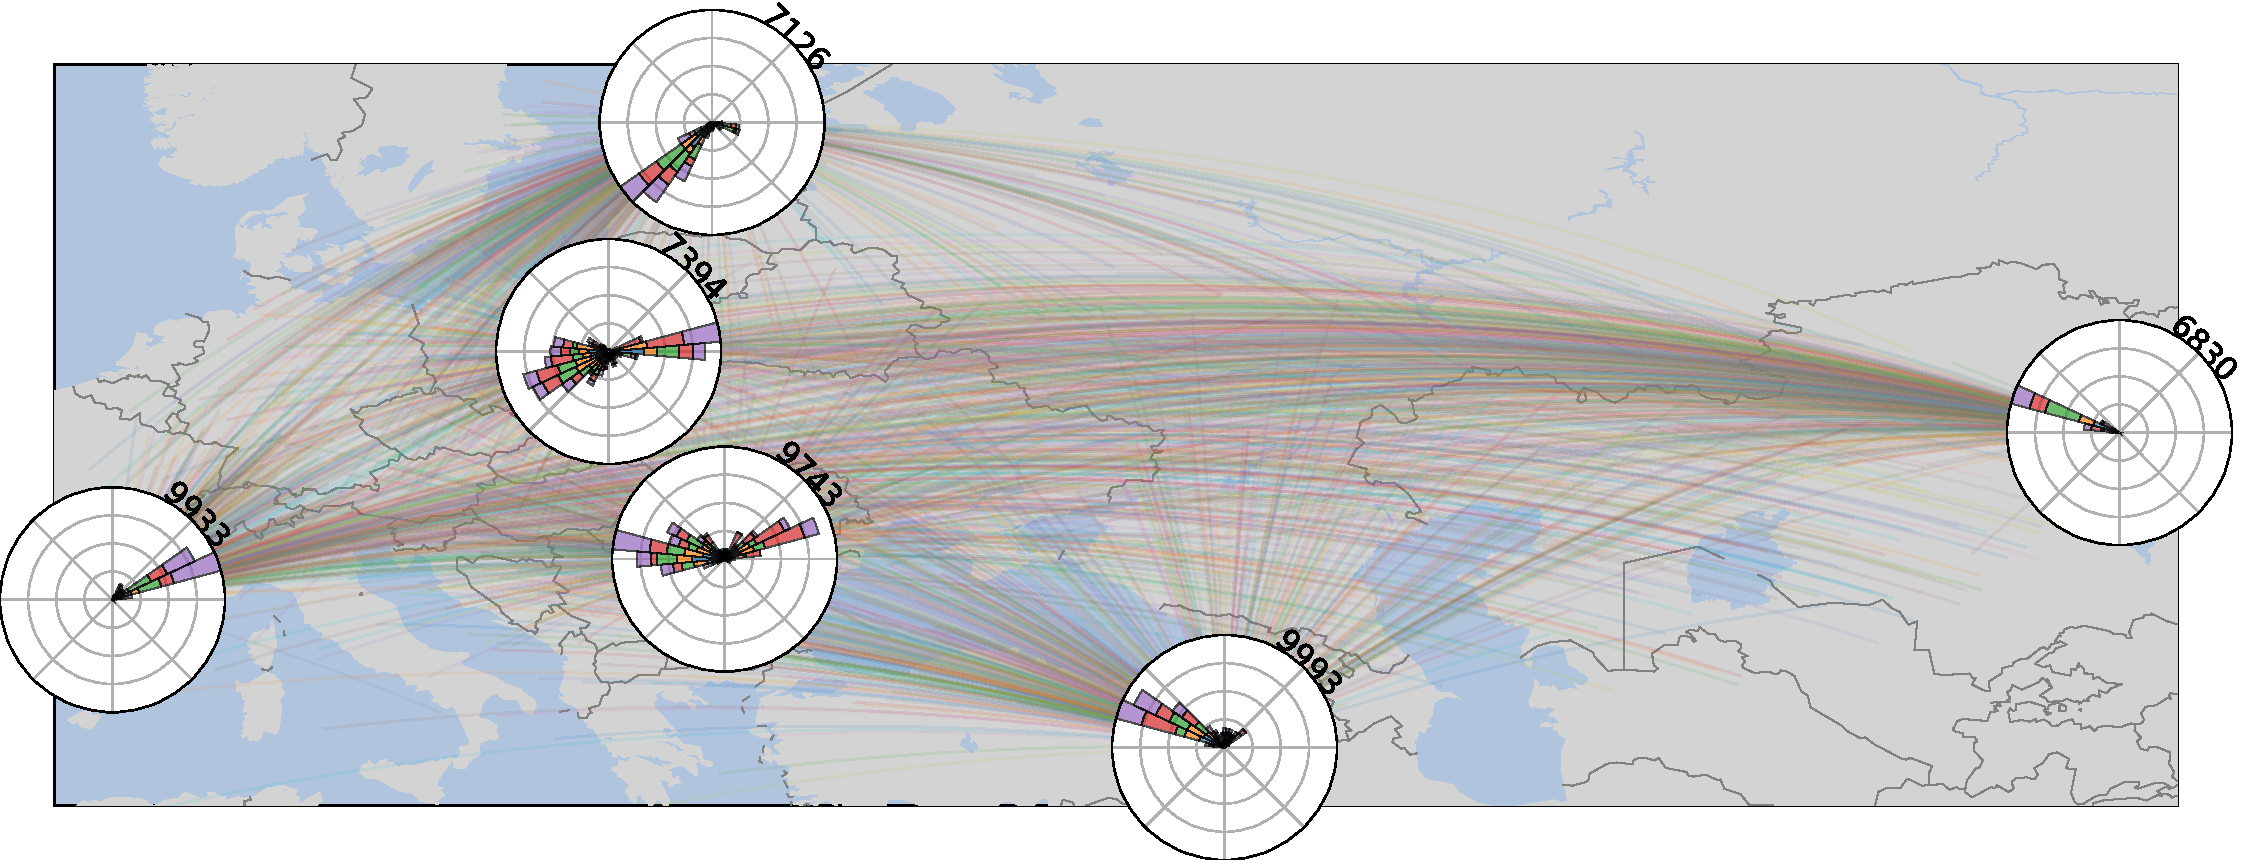
\includegraphics[width=\linewidth]{plots/1001G_windrose_admixed_weighted.pdf}
  };
  \node[anchor = north west] at ($(A.north west) + (0.5, -0.5)$) {
    \textbf{A}
  };

% genomes
  \node[below = 0cm of A] (B) {  
    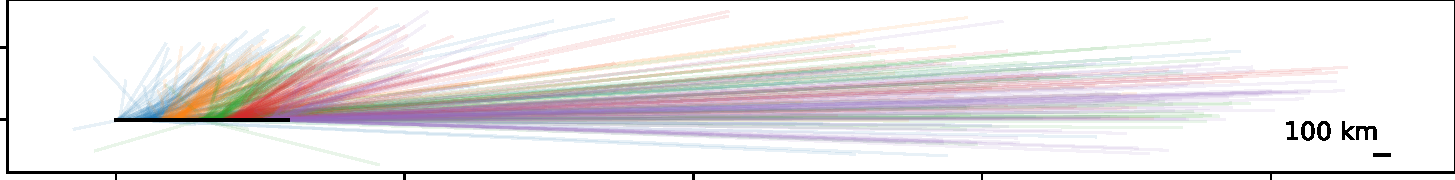
\includegraphics[width=1\linewidth]{{plots/1001G_genome-displacements_tsplits[10,100,1000]_node1044_time10.pdf}}
  };
  \node[anchor = north west] at ($(B.north west) + (0.2,-0.1)$) {
    \footnotesize 9933
  };
  \node[below = 0cm of B, text width = \linewidth] (C) {  
    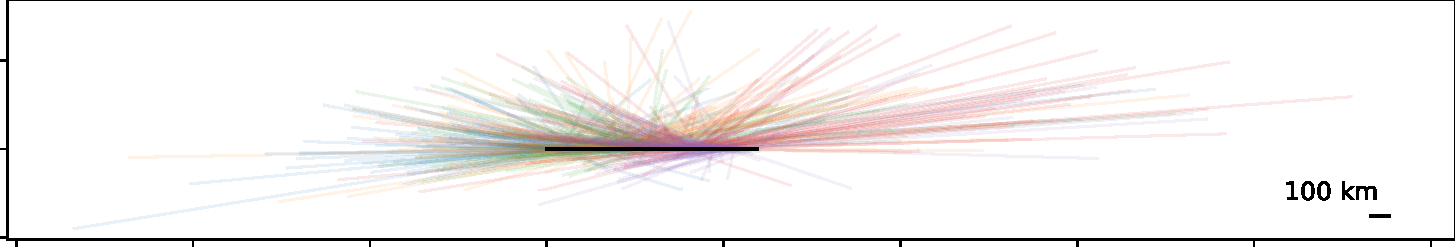
\includegraphics[width=1\linewidth]{{plots/1001G_genome-displacements_tsplits[10,100,1000]_node881_time10.pdf}}
  };
  \node[anchor = north west] at ($(C.north west) + (0.2,-0.1)$) {
    \footnotesize 9743
  };
  \node[anchor = south west] at ($(B.north west) + (0.5, -0.1)$) {
    \textbf{B}
  };
  
  
\end{tikzpicture}  

\end{center}

\caption{
\textbf{Locating genetic ancestors to visualize admixture and its sources}.
\textbf{(A)} The curves on the map are great circle paths connecting the sample locations (center of `windrose' insets) to the maximum likelihood ancestor locations 10 generations ago at $10^2$ evenly-spaced loci per chromosome for 6 striking Admixed samples (accession numbers as labels).
The windrose insets show a histogram of directions from the sample to the ancestors, weighted by distance.
Colours indicate chromosomes, as in Figure \ref{fig:thal_sigma}.
\textbf{(B)} The black horizontal line represents the genome and the coloured lines show the ancestral displacements in longitude and latitude (converted to kms) from that position of the genome.
See Figure \ref{fig:thal_admixed_genome_displacements} for the genome-view of ancestral displacements of all 6 samples.
Maximum likelihood locations calculated using per-chromosome four-epoch dispersal rates (Figure \ref{fig:thal_sigma}B).
}

\label{fig:thal_chr_displaced}
\end{figure}

There is also information contained in the correlation of ancestral movements across the genome. 
To demonstrate how geographic ancestries are correlated across the genome, Figure \ref{fig:thal_chr_displaced}B shows each displacement emanating from it's location along a linear representation of the genome (rather than all emanating from the same place, as in the map) for the French and Romanian sample (see Figure \ref{fig:thal_admixed_genome_displacements} for the other 4 samples).
With this visual we see that the French sample gets much of its most eastern ancestry from chromosomes 3 and 5 (green and purple) while the Romanian sample gets most of its eastern ancestry from chromosome 4 (red).
This figure also serves to illustrate just how much information is being inferred -- at any time in the past, we can estimate the locations of thousands of genetic ancestors for thousands of samples, providing a rich source of information to explore and use to test hypotheses.

%%%%%%%%%%%%%%%%%%%%%%%%%%%%%%%%%%%%%%%%%%%%%%%%%
%%%%%%%%%%%%%%%%%%%%%%%%%%%%%%%%%%%%%%%%%%%%%%%%%
\section*{Discussion}
%%%%%%%%%%%%%%%%%%%%%%%%%%%%%%%%%%%%%%%%%%%%%%%%%
%%%%%%%%%%%%%%%%%%%%%%%%%%%%%%%%%%%%%%%%%%%%%%%%%

%%%%%%%%%%%%%%%%%%%%%%%%%%%%%%%%%%%%%%%%%%%%%%%%%
\subsection*{Summary of main results}

We have developed a method that uses a sequence of trees along a recombining genome -- a genome-wide genealogy -- to estimate individual-level dispersal rates and locate genetic ancestors (Figure \ref{fig:overview}). 
At the core of our method is a simple model of Brownian motion, allowing likelihoods to be quickly calculated from shared evolutionary times and sample locations.
On top of this we layer on importance sampling to correct for bias in inferred branch lengths, a time cutoff to ignore strong violations of the model in the deep past, and multiple epochs to allow the dispersal rate to vary through time. 
Simulation tests show that our method can accurately infer dispersal rate (with a slight overestimate caused by errors in tree inference), detect shifts in the dispersal rate over time, and trace major geographic ancestries hundreds of generations into the past (Figure \ref{fig:sims}).
Applying our method to more than one thousand \textit{Arabidopsis thaliana} genomes across a huge geographic expanse \citep{alonso2016}, we find strong evidence for very rapid recent dispersal (Figure \ref{fig:thal_sigma}), especially across longitude, and show how locating genetic ancestors can detect and visualize \textit{i}) long-distance dispersal events (Figures \ref{fig:thal_displaced}-\ref{fig:thal_outliers}), \textit{ii}) the source of population expansions (Figure \ref{fig:thal_NA}), \textit{iii}) alternative geographic ancestries (Figures \ref{fig:thal_ancestries}-\ref{fig:thal_spanish_moves}), and \textit{iv}) admixture (Figure \ref{fig:thal_chr_displaced}).

%%%%%%%%%%%%%%%%%%%%%%%%%%%%%%%%%%%%%%%%%%%%%%%%%
\subsection*{Comparison with previous methods}

% history
The idea of using trees to estimate continuous ancestral characters and their rate of change is an old one.
This was originally applied to population-level characters, such as the frequency of genes in a population and their rate of genetic drift, in a phylogenetic context \citep{cavalli1964analysis,cavalli1967phylogenetic,edwards1970estimation,felsenstein1973maximum,felsenstein1985phylogenies,grafen1989phylogenetic}.
DNA sequencing later allowed the inference of a single tree relating individual samples for a sufficiently long non-recombining sequence (as found on the human Y chromosome, in a mitochondrial genome, or in the nuclear genome of a predominately non-recombining species), which led to estimates of dispersal rates and ancestral locations under the banner of `phylogeography' 
\citep{avise2009phylogeography,knowles2009statistical}.
Phylogeography has proven incredibly useful, especially to infer the geographic origin and spread of viruses \citep{biek2007high,lemey2009bayesian,lemey2010phylogeography,bedford2010global,volz2013viral}, such as SARS-CoV-2 \citep{worobey2020emergence,lemey2020accommodating,dellicour2021phylodynamic,dellicour2021dispersal,martin2021insights}.
% tree sequences
Extending phylogeography to frequently-recombining sequences is not straightforward as there are then many true trees that relate the samples.
Only recently has it become feasible to infer the sequence of trees, and their branch lengths, along a recombining genome \citep{rasmussen2014genome,speidel2019method,wohns2021unified}.
Our method capitalizes on this advance to use some of the enormous amount of information contained in a tree sequence of a large sample in a recombining species.

% wohns
A related method was recently demonstrated by \cite{wohns2021unified}, who inferred the geographic location of coalescent nodes in a \texttt{tskit} tree sequence \citep{kelleher2018efficient}, where information about nodes and branches are shared between trees.
Our approach differs from theirs in a number of ways. 
First, they utilize the sharing of information about nodes and branches across trees to very efficiently geographically locate every node exactly once, by locating a `parent' node at the midpoint between its two `child' nodes geographic locations and iterating up the entire tree sequence simultaneously (rather than up each local tree individually).
In addition to being fast this has the advantage of using information from all the trees in a tree sequence.
In contrast, we locate ancestors independently at each local tree we consider.
As some ancestors (represented as nodes and branches) are shared between nearby trees along the genome (though we don't know precisely for how long since we lose that information when converting the \texttt{Relate}-inferred genealogy into a tree sequence), we avoid locating the same ancestors multiple times by using only a sample of the trees (e.g., for \textit{A.\ thaliana} we uniformly sampled 5000 of the $\sim$200,000 trees, $\sim2.5\%$).
Our approach therefore uses less of the information in the tree sequence, in this sense.
(Note that while we choose trees that have low linkage disequilibrium with one another and are therefore essentially unlinked, in the very recent past they will share ancestors but will quickly become independent \citep{wakeley2012gene}.)
On the other hand, when locating an ancestor we not only use information `below' this ancestor (i.e., its descendants' locations and relations) but also the information `above' the ancestor, due to the ancestor's lineage sharing evolutionary time and a recent common ancestor with non-descendant lineages.
Further advantages of our method include the ability to estimate dispersal rates and uncertainties in ancestor locations (as we have taken a parametric approach), the ability to locate ancestors at any time (not just at coalescent nodes but also at any point along a branch), and accounting for uncertainty in the branch lengths (using importance sampling; this could be extended to capture uncertainty in the topologies as well once they can be efficiently sampled).

%ARGs
An exciting possibility is a merger of these two methods, to efficiently use information from all the trees in the tree sequence and all the information above and below ancestors. 
One approach might be to use something like the inside-outside algorithm in \citep{wohns2021unified}, which they use for node times but not locations.
A second approach would be to model Brownian motion on the full ancestral recombination graph \citep[e.g. using a program like \texttt{ARGweaver;}][]{rasmussen2014genome}. 
The latter approach would allow one to visualize the geographic splitting and coalescence of the ancestors of a genome backwards in time.

%%%%%%%%%%%%%%%%%%%%%%%%%%%%%%%%%%%%%%%%%%%%%%%%%
\subsection*{Future directions}

% alternative likelihood models
We have chosen to stick with a very simple model of Brownian motion with a piecewise-constant dispersal rate over time.
There are a number of extensions that could readily be applied.
For instance, we could allow dispersal rates to vary between branches \citep{o2006testing}, e.g., to compare dispersal rates in different parts of a species' range.
Or we could model dispersal under a more complex model, like the Early Burst \citep{harmon2010early} or a L{\'e}vy process 
\citep{landis2013phylogenetic}, which may help identify periods of range expansion or sudden long-range dispersal.
% Bayesian models
Alternatively we could take a Bayesian approach, allowing much greater flexibility and the incorporation of many recent advances in phylogeography.
For example, one could then model dispersal as a relaxed random walk \citep{lemey2010phylogeography}, which may be more appropriate for sample locations that are very non-normal and could incorporate habitat boundaries.
Second, given that there is large variance in the inferred locations of distant ancestors at any one locus \citep{schluter1997likelihood}, but very many loci, we could take an `empirical Bayes' approach and use the posteriors on ancestral locations over many loci to set a prior for a given locus.
This might be especially helpful at deeper times, e.g., tracing human ancestors back 100s of thousands of years, where the noise in the ancestral location at any one locus is large, yet we can be relatively certain that the majority of lineages are in Africa.
We might alternatively set priors to test hypotheses, e.g., if we surmise there were multiple glacial refugia during the last glaciation we can set a prior on ancestral location with peaks at these hypothesized locations and infer what percent of a sample's lineages descended from each.
Models of ancestral locations based on past climatic- and ecological-niche models could provide a rich source of data for building such priors, and given the large amounts data available in recombining sequences these models could be subject to rigorous model choice.
% machine learning
Finally, it might also be interesting to take a more model-agnostic approach and use machine learning.
For example, \texttt{Locator} \citep{battey2020predicting} uses deep neural networks to infer the locations of extant individuals from unphased genotype data.
In essence this means \texttt{Locator} is both determining the relationships between samples and locating them.
Separating these two steps by first inferring a tree sequence and then supplying information from this tree sequence to the deep neural network may both improve location estimates for extant individuals and allow such a method to locate genetic ancestors.

% ancient samples
Our approach relies on the locations of the current-day samples. 
While we have shown that we can learn much about the geographical history of a species with this approach, its accuracy is necessarily limited. 
For example, if historical parts of the range are undersampled in a particular dataset the method will struggle to locate ancestors in these regions, particularly further into the past, as we saw with the Iberian Relicit samples with ancestry from the putative north African refugia.
Similarly, if a species' range has shifted such that few present day individuals exist in portions of the historic range, we will often not infer ancestors to be in the currently sparsely-occupied portions. 
Other large scale population movements, such as one population replacing another, may also partially obscure the geographic locations of ancestors. 
Over the past decade we have learned about numerous large-scale movements of human populations alongside the expansions of archaeological cultures, a fact fairly hidden from view by contemporary samples that only ancient DNA could bring to light \citep{slatkin2016ancient,reich2018we}.
One obvious way to improve our method then, is to include ancient samples. 
Given that it is now possible to include high-coverage ancient genomes in tree sequences \citep{speidel2021inferring,wohns2021unified}, it is straightforward to include this information in our likelihoods (ancient samples are treated as any other, we calculate the shared times of these lineages with themselves and with all other sample lineages), influencing both our dispersal estimates and inferred ancestral locations.
This should help, in particular, in locating ancestors that are closely related to the ancient samples and for detecting population-scale movements, such as range shifts, contractions, and replacements.

%%%%%%%%%%%%%%%%%%%%%%%%%%%%%%%%%%%%%%%%%%%%%%%%%
%%%%%%%%%%%%%%%%%%%%%%%%%%%%%%%%%%%%%%%%%%%%%%%%%
\section*{Materials and Methods}
\label{sec:methods}
%%%%%%%%%%%%%%%%%%%%%%%%%%%%%%%%%%%%%%%%%%%%%%%%%
%%%%%%%%%%%%%%%%%%%%%%%%%%%%%%%%%%%%%%%%%%%%%%%%%

Here we describe our methods to estimate dispersal rates and locate genetic ancestors and how we applied these to simulations and \textit{Arabidopsis thaliana}.

%%%%%%%%%%%%%%%%%%%%%%%%%%%%%%%%%%%%%%%%%%%%%%%%%
\subsection*{The probability of the sampled locations given a tree and the dispersal rate}
%%%%%%%%%%%%%%%%%%%%%%%%%%%%%%%%%%%%%%%%%%%%%%%%%

We first derive the probability of the sampled locations, $\mathbf{L}$, given a bifurcating tree topology (genealogy), $\mathcal{G}$, and associated branch lengths (times), $\mathcal{T}$, which describe the coalescent history of the sample, and the dispersal rate (covariance matrix), $\mathbf{\Sigma}$. 
We derive this probability, $\mathbb{P}(\mathbf{L} | \mathcal{G},\mathcal{T},\mathbf{\Sigma})$, compounding the normally-distributed dispersal events each generation to give Brownian motion down the tree in a similar manner to phylogenetic least squares regression \citep{grafen1989phylogenetic,harmon2019phylogenetic}.

Let $\bm{\ell}_i = [\ell_{i,1} \; \ell_{i,2} \; ... \;\ell_{i,m}]^\intercal$ be the $m$-dimensional location of sample $i$, $\mathbf{L} = [\bm{\ell}_1\; \bm{\ell}_2\; \dots \; \bm{\ell}_n]^\intercal$ the $n\times m$ matrix of spatial locations for all $n$ samples, and $\bm{\ell} = [\ell_{1,1} \; \ell_{2,1} \; ... \; \ell_{n,1} \; \ell_{1,2} \; \ell_{2,2} \; ... \; \ell_{n,2} \; ... \; \ell_{1,m} \; \ell_{2,m} \; ... \; \ell_{n,m}]^\intercal$ the matrix of locations represented as a vector of length $nm$.
Let $\mathbf{S}_{\mathcal{G},\mathcal{T}}$ be the $n\times n$ matrix of shared evolutionary time (in generations) between each sample lineage in the tree defined by $\mathcal{G}$ and $\mathcal{T}$.

Then, assuming per generation dispersal is multivariate normal with mean displacement $\mathbf{0}$ and covariance matrix $\mathbf{\Sigma}$, the probability of the locations given the tree is
%
\begin{equation}\label{eq:PS}
\mathbb{P}(\mathbf{L} | \mathcal{G},\mathcal{T}, \mathbf{\Sigma}) = \mathbb{P}(\bm{\ell} | \mathbf{S}_{\mathcal{G},\mathcal{T}}, \mathbf{\Sigma}) \sim \mathcal{N}\left(\mathbf{D} \widehat{\bm{\ell}_A}, \mathbf{S}_{\mathcal{G},\mathcal{T}} \otimes \mathbf{\Sigma} \right),
\end{equation}
%
where
%
\begin{equation}\label{eq:sa}
\widehat{\bm{\ell}_A} = [(\mathbf{1}^\intercal \mathbf{S}_{\mathcal{G},\mathcal{T}}^{-1} \mathbf{1})^{-1}(\mathbf{1}^\intercal \mathbf{S}_{\mathcal{G},\mathcal{T}}^{-1} \mathbf{L})]^\intercal
\end{equation}
%
is the maximum likelihood estimate for the location of the most recent common ancestor given the tree, $\mathbf{1}$ is a column vector of $n$ ones, and $\mathbf{D}$ is a $nm\times m$ design matrix whose $i,j^\mathrm{th}$ entry is 1 if $(j-1) n < i \leq j n$ and 0 otherwise.

%%%%%%%%%%%%%%%%%%%%%%%%%%%%%%%%%%%%%%%%%%%%%%%%%
\subsubsection*{Mean centering the locations}
%%%%%%%%%%%%%%%%%%%%%%%%%%%%%%%%%%%%%%%%%%%%%%%%%

We can remove any dependence on the (unknown) location of the most recent common ancestor by mean centering the data. 
The mean centered locations and associated matrix of shared times are $\mathbf{X}=\mathbf{M}\mathbf{L}$ and $\mathbf{V}_{\mathcal{G},\mathcal{T}}=\mathbf{M}\mathbf{S}_{\mathcal{G},\mathcal{T}}\mathbf{M}^\intercal$, where $\mathbf{M}$ is an $(n-1)\times n$ matrix with $n-1/n$ on the diagonal and $-1/n$ elsewhere. %= n \mathbf{I} - \tfrac{1}{n}\mathbf{1}^\intercal \mathbf{1}$ with $\mathbf{I}$ an $n\times n$ identity matrix.
We only use those (sub)trees (see below) with $n>1$ samples (i.e., trees with only one sample contain no information about the dispersal rate if we do not know where the ancestor was).
We then have
%
\begin{equation}\label{eq:PScentered}
\mathbb{P}(\mathbf{X} | \mathcal{G},\mathcal{T}, \mathbf{\Sigma}) = \mathbb{P}(\mathbf{x} | \mathbf{V}_{\mathcal{G},\mathcal{T}}, \mathbf{\Sigma}) \sim \mathcal{N}\left(\mathbf{0}, \mathbf{V}_{\mathcal{G},\mathcal{T}} \otimes \mathbf{\Sigma} \right),
\end{equation}
%
where $\mathbf{x}$ is the vector representation of $\mathbf{X}$ (as $\bm{\ell}$ is to $\mathbf{L}$).


%%%%%%%%%%%%%%%%%%%%%%%%%%%%%%%%%%%%%%%%%%%%%%%%%
\subsubsection*{Chopping the tree into subtrees}
%%%%%%%%%%%%%%%%%%%%%%%%%%%%%%%%%%%%%%%%%%%%%%%%%

We will usually want to only consider dispersal more recently than some cutoff time, $T$, since deeper genealogical history may contain little geographic information \citep{wilkins2004separation}.
When this is the case we cut the full tree of at $T$, leaving us with $n_T \in [1, n ] $ subtrees, where all coalescent times are $<T$, and we then calculate the shared times in each subtree independently.
Letting $\mathbb{P}(\mathbf{x}_i | \mathbf{V}_{\mathcal{G}_i,\mathcal{T}_i}, \mathbf{\Sigma})$ be the probability of the (mean centered and vectorized) locations of the samples in subtree $i$ given the (mean centered) matrix of shared evolutionary times in that subtree and the dispersal rate, the probability of the locations of all samples is
%
\begin{equation}\label{eq:PScentered_chopped}
\mathbb{P}(\mathbf{X} | \mathcal{G},\mathcal{T}, \mathbf{\Sigma}, T) = \prod_{i=1}^{n_T} \mathbb{P}(\mathbf{x}_i | \mathbf{V}_{\mathcal{G}_i,\mathcal{T}_i}, \mathbf{\Sigma}) \sim \prod_{i=1}^{n_T} \mathcal{N}\left(\mathbf{0}, \mathbf{V}_{\mathcal{G}_i,\mathcal{T}_i} \otimes \mathbf{\Sigma} \right). %= \mathcal{N}\left(\mathbf{0}, \mathbf{V}_{\mathcal{G},\mathcal{T}}_T \otimes \mathbf{\Sigma} \right),
\end{equation} 
This has the added benefit of expressing the probability as a function of smaller submatrices of shared evolutionary times, which are faster to invert.
%where $\mathbf{V}_{\mathcal{G},\mathcal{T}}_T = \sum_{i=1}^{\eta} \mathbf{V}_{\mathcal{G},\mathcal{T}}_i^{-1}$.

%%%%%%%%%%%%%%%%%%%%%%%%%%%%%%%%%%%%%%%%%%%%%%%%%
\subsubsection*{Dividing time into epochs}
%%%%%%%%%%%%%%%%%%%%%%%%%%%%%%%%%%%%%%%%%%%%%%%%%

We can extend this model to allow dispersal to vary through time by dividing time into epochs and assuming dispersal is only constant within each. 
If we divide time into $K$ epochs (as described by a vector of split times, $\mathbf{t}$), so that the (mean centered) shared time matrix in the $i^\mathrm{th}$ epoch is $\mathbf{V}_{\mathcal{G},\mathcal{T}}^{(i)}$, then
%
\begin{equation}\label{eq:PScentered_epochs}
\begin{aligned}
\mathbb{P}(\mathbf{X} | \mathcal{G},\mathcal{T}, \mathbf{\Sigma}_1, ..., \mathbf{\Sigma}_K, \mathbf{t}) &= \mathbb{P}(\mathbf{x} | \mathbf{V}_{\mathcal{G},\mathcal{T}}^{(1)}, ..., \mathbf{V}_{\mathcal{G},\mathcal{T}}^{(E)}, \mathbf{\Sigma}_1, ..., \mathbf{\Sigma}_E)\\
& \sim \mathcal{N}\left(\mathbf{0}, \sum_{i=1}^{K} ( \mathbf{V}_{\mathcal{G},\mathcal{T}}^{(i)} \otimes \mathbf{\Sigma}_i ) \right).
\end{aligned}
\end{equation}
Thus different dispersal epochs are easily accounted for.

%%%%%%%%%%%%%%%%%%%%%%%%%%%%%%%%%%%%%%%%%%%%%%%%% 
\subsubsection*{Importance sampling}
%%%%%%%%%%%%%%%%%%%%%%%%%%%%%%%%%%%%%%%%%%%%%%%%%

The calculations above, which give the likelihood of the dispersal rate given the sample locations, were all predicated on knowing the tree with certainty, which will not be the case when inferring trees from genetic data.
Further, inferring a tree may involve assumptions (such as panmixia) that are inconsistent with the model we are using.
To deal with the uncertainty and bias we calculate the likelihood of our parameters given the data using importance sampling, a likelihood ratio, and Monte Carlo approximation.
Importance sampling corrects the expectation of the likelihood by reweighting draws from an `incorrect' (proposal) distribution to match the `correct' (target) distribution. 
These importance weights downweight draws from the proposal distribution that are likely under the proposal distribution but unlikely under the target distribution and upweight draws that are likely in the target distribution and unlikely under the proposal distribution. 
Importance sampling techniques to sample genealogies in population genetics have been applied a number of settings as coalescent models provide convenient priors on trees and it is often challenging to sample genealogies consistent with data \citep{griffiths1997computational,stephens2000inference,meligkotsidou2007postprocessing}. 
See \cite{stern2019approximate,stern2020disentangling} for recent applications of these ideas to marginal trees inferred along a recombining sequence, whose general approach we follow below.  

The data we have are the locations of the samples, $\mathbf{L}$, and their haplotypes, $\mathbf{H}$.
From this data we want to infer two unknowns, a tree topology, $\mathcal{G}$, and associated branch lengths, $\mathcal{T}$, and use these to estimate the likelihood the dispersal rate, $\mathbf{\Sigma}$.
Put another way, we want to estimate $\mathbb{E}_{\mathcal{G},\mathcal{T} | \mathbf{\Sigma}} \left[ \mathbb{P}(\mathbf{L},\mathbf{H} | \mathcal{G},\mathcal{T},\mathbf{\Sigma}) \right]$, which is the likelihood of our parameters given the data, integrated over the unknowns. 

Current methods to infer tree topologies and times along a recombining sequence \citep{rasmussen2014genome,speidel2019method,kelleher2019inferring,wohns2021unified} assume panmictic, well-mixed populations. 
This implies we cannot sample topologies and branch lengths, $\mathcal{G}$ and $\mathcal{T}$, under our spatial model, creating potential bias.
To correct for this bias we use importance sampling,
%
\begin{equation}
\begin{aligned}
\mathrm{L}(\mathbf{\Sigma}) &:= \mathbb{E}_{\mathcal{G}, \mathcal{T} | \mathbf{\Sigma}} \left[ \mathbb{P}(\mathbf{L},\mathbf{H} | \mathcal{G},\mathcal{T},\mathbf{\Sigma}) \right] \\
&= \mathbb{E}_{ \mathcal{G}, \mathcal{T} | \mathbf{H}, \mathrm{panmixia}} \left[ \frac{\mathbb{P}(\mathbf{L},\mathbf{H} | \mathcal{G}, \mathcal{T},\mathbf{\Sigma}) \mathbb{P}(\mathcal{G}, \mathcal{T} | \mathbf{\Sigma})}{\mathbb{P}(\mathcal{G}, \mathcal{T} | \mathbf{H}, \mathrm{panmixia})} \right],
\end{aligned}
\end{equation}
%
where $\mathbb{P}(\mathcal{G}, \mathcal{T} | \mathbf{H}, \mathrm{panmixia})$ is the distribution of topologies and branch lengths we sample from.

The probabilities containing the genetic data, $\mathbf{H}$, are complicated to calculate. 
To simplify we divide by the likelihood of panmixia given the data, $\mathrm{L}(\mathrm{panmixia}) = \mathbb{P}(\mathbf{H}|\mathrm{panmixia})$, to work with the likelihood ratio
%
\begin{equation}
\begin{aligned}
\mathrm{LR}(\mathbf{\Sigma}) &:= \frac{\mathrm{L}(\mathbf{\Sigma})}{\mathrm{L}(\mathrm{panmixia})}\\
&= \mathbb{E}_{\mathcal{G}, \mathcal{T} | \mathbf{H}, \mathrm{panmixia}} \left[ \frac{\mathbb{P}(\mathbf{L}, \mathbf{H} | \mathcal{G}, \mathcal{T},\mathbf{\Sigma}) \mathbb{P}(\mathcal{G}, \mathcal{T} | \mathbf{\Sigma})}{\mathbb{P}(\mathcal{G}, \mathcal{T} | \mathbf{H}, \mathrm{panmixia}) \mathbb{P}(\mathbf{H} | \mathrm{panmixia})} \right] \\
&= \mathbb{E}_{\mathcal{G}, \mathcal{T} | \mathbf{H}, \mathrm{panmixia}} \left[ \frac{\mathbb{P}(\mathbf{L},\mathbf{H} | \mathcal{G}, \mathcal{T},\mathbf{\Sigma}) \mathbb{P}(\mathcal{G}, \mathcal{T} | \mathbf{\Sigma})}{\mathbb{P}(\mathbf{H}, \mathcal{G}, \mathcal{T} | \mathrm{panmixia})} \right] \\
&= \mathbb{E}_{\mathcal{G}, \mathcal{T} | \mathbf{H}, \mathrm{panmixia}} \left[ \frac{\mathbb{P}(\mathbf{H} | \mathcal{G}, \mathcal{T}) \mathbb{P}(\mathbf{L} | \mathcal{G}, \mathcal{T},\mathbf{\Sigma}) \mathbb{P}(\mathcal{G}, \mathcal{T} | \mathbf{\Sigma})}{\mathbb{P}(\mathbf{H} | \mathcal{G},\mathcal{T})\mathbb{P}(\mathcal{G}, \mathcal{T} | \mathrm{panmixia})} \right] \\
&= \mathbb{E}_{\mathcal{G}, \mathcal{T} | \mathbf{H}, \mathrm{panmixia}} \left[ \frac{ \mathbb{P}(\mathbf{L} | \mathcal{G}, \mathcal{T}, \mathbf{\Sigma}) \mathbb{P}(\mathcal{G}, \mathcal{T} | \mathbf{\Sigma})}{\mathbb{P}(\mathcal{G}, \mathcal{T} | \mathrm{panmixia})} \right],
%&= \mathbb{E}_{T|\mathbf{H},G,\mathrm{panmixia}} \left[ \frac{ \mathbb{P}(\mathbf{L}, T | G, P)}{\mathbb{P}(\mathcal{T} | \mathcal{G},\mathrm{panmixia})} \right],
\end{aligned}
\end{equation}
%
where the third step assumes the genetic data ($\mathbf{H}$) is conditionally independent of the spatial parameters ($\mathbf{\Sigma}$ or panmixia) and locations ($\mathbf{L}$) given the tree ($\mathcal{G}$ and $\mathcal{T}$).
We can approximate this expectation using Monte Carlo sampling
%
\begin{equation}\label{eq:LRmontecarlo1}
\widehat{\mathrm{LR}(\mathbf{\Sigma})} = \frac{1}{M} \sum_{m=1}^{M} \frac{ \mathbb{P}(\mathbf{L} | \mathcal{G}_m, \mathcal{T}_m, \mathbf{\Sigma}) \mathbb{P}(\mathcal{G}_m, \mathcal{T}_m | \mathbf{\Sigma})}{\mathbb{P}(\mathcal{G}_m, \mathcal{T}_m | \mathrm{panmixia})},
\end{equation}
%
where $\mathcal{G}_m, \mathcal{T}_m \sim \mathbb{P}(\mathcal{G}, \mathcal{T} | \mathbf{H}, \mathrm{panmixia})$ is sampled using Markov chain Monte Carlo.

We make two final simplifications.
First, we will use a model of branching Brownian motion for $\mathbb{P}(\mathcal{G}, \mathcal{T} | \mathbf{\Sigma})$ and the standard neutral coalescent for $\mathbb{P}(\mathcal{G}, \mathcal{T} | \mathrm{panmixia})$.
Under both of these models the probability of the topology, $\mathbb{P}(\mathcal{G} | \mathrm{panmixia})$, is equivalent (and uniform).
Second, we will use \texttt{Relate} \citep{speidel2019method} to infer topologies and branch lengths.
\texttt{Relate} returns a single topology and allows resampling over branch lengths conditional on this topology.
We therefore take the topology as given and integrate only over branch lengths.
Putting these two simplifications together,
%
\begin{equation}\label{eq:LRmontecarlo}
\begin{aligned}
\widehat{\mathrm{LR}(\mathbf{\Sigma})} &= \frac{1}{M} \sum_{m=1}^{M} \frac{ \mathbb{P}(\mathbf{L} | \mathcal{G}_m, \mathcal{T}_m, \mathbf{\Sigma}) \mathbb{P}(\mathcal{G}_m, \mathcal{T}_m | \mathbf{\Sigma})}{\mathbb{P}(\mathcal{G}_m, \mathcal{T}_m | \mathrm{panmixia})}\\
&= \frac{1}{M} \sum_{m=1}^{M} \frac{ \mathbb{P}(\mathbf{L} | \mathcal{G}_m, \mathcal{T}_m, \mathbf{\Sigma}) \mathbb{P}(\mathcal{T}_m | \mathcal{G}_m, \mathbf{\Sigma}) \mathbb{P}(\mathcal{G}_m | \mathbf{\Sigma})}{\mathbb{P}(\mathcal{T}_m | \mathcal{G}_m, \mathrm{panmixia}) \mathbb{P}(\mathcal{G}_m | \mathrm{panmixia})}\\
&= \frac{1}{M} \sum_{m=1}^{M} \frac{ \mathbb{P}(\mathbf{L} | \mathcal{G}_m, \mathcal{T}_m, \mathbf{\Sigma}) \mathbb{P}(\mathcal{T}_m | \mathcal{G}_m, \mathbf{\Sigma})}{\mathbb{P}(\mathcal{T}_m | \mathcal{G}_m, \mathrm{panmixia}) }\\
&\approx \frac{1}{M} \sum_{m=1}^{M} \frac{ \mathbb{P}(\mathbf{L} | \mathcal{G}, \mathcal{T}_m, \mathbf{\Sigma}) \mathbb{P}(\mathcal{T}_m | \mathcal{G}, \mathbf{\Sigma})}{\mathbb{P}(\mathcal{T}_m | \mathcal{G}, \mathrm{panmixia})},
\end{aligned}
\end{equation}
%
where $\mathcal{T}_m \sim \mathbb{P}(\mathcal{T} | \mathbf{H}, \mathrm{panmixia}, \mathcal{G})$ is sampled using Markov chain Monte Carlo.
Note that because the probability of a topology is the same in the two models, and therefore cancels out, our method can immediately be extended to integrate over both topologies and branch lengths.


To find the maximum likelihood estimate of $\mathbf{\Sigma}$ we numerically search for the $\mathbf{\Sigma}$ that maximizes this likelihood ratio. 
We measure the variance around this estimate with the Hessian matrix of the likelihood surface returned by the numerical search. 
To use information from multiple loci, e.g., to estimate a per-chromosome or genome-wide dispersal parameter, we can multiply the likelihood ratios together to give a composite likelihood ratio.
This is a composite likelihood because it ignores correlations in the trees between loci \citep{hudson2001two,larribe2011composite,varin2011overview}. The maximum likelihood of genome-wide parameters from composite likelihood are known to be statistically consistent in the presence of such correlations \citep{wiuf2006consistency}, but the likelihood surface is overly peaked due to ignoring the correlations in the data. 
However, in practice we take loci that are far enough apart that their trees are only weakly correlated more than a few tens of generations back.

We next show how we derive the probability distributions of the branch lengths in the tree that we use as the weights in the importance sampler, $\mathbb{P}(\mathcal{T} | \mathcal{G}, \mathrm{panmixia})$ and $\mathbb{P}(\mathcal{T} | \mathcal{G}, \mathbf{\Sigma})$.

%%%%%%%%%%%%%%%%%%%%%%%%%%%%%%%%%%%%%%%%%%%%%%%%%
\subsubsection*{The probability of the coalescence times given the tree topology and panmixia}
%%%%%%%%%%%%%%%%%%%%%%%%%%%%%%%%%%%%%%%%%%%%%%%%%

\texttt{Relate} and other tree construction methods infer the times in the trees under a model of panmixia with variable population size through time (with this demographic history inferred genomes as part of the method). 
The probability of the coalescence times given the tree topology and panmixia, $\mathbb{P}(\mathcal{T} | \mathcal{G}, \mathrm{panmixia})$, can be derived from the standard neutral coalescent allowing for (stepwise) changing effective population size \citep{griffiths1994sampling,meligkotsidou2007postprocessing}.
 
Let the number of samples be $n$ and let $\mathbf{U}$ be the $n-1$ coalescence times, ordered from most recent to most historic.
Then
%
\begin{equation}
\mathbb{P}(\mathcal{T} | \mathcal{G},\mathrm{panmixia}) = \prod_{i=1}^{n-1} \mathbb{P}(U_i = u_i | U_{i-1} = u_{i-1}),
\end{equation}
%
where
%
\begin{equation}
\begin{aligned}
& \mathbb{P}(U_i = u_i | U_{i-1} = u_{i-1})\\
& = \binom{n-(i-1)}{2}\frac{1}{2N(u_i)}\exp\left[ -\binom{n-(i-1)}{2} [\Lambda(u_i) - \Lambda(u_{i-1})] \right]
\end{aligned}
\end{equation}
%
with
%
\begin{equation}
\Lambda(u) = \int_0^u \frac{1}{2N(t)} \mathrm{d}t,
\end{equation}
%
where $N(t)$ is the effective population size at time $t$ in the past.

This says that the coalescence times are produced by a Markov process, so that the probability of the $i^{th}$ coalescence being at time $u_i$ is independent of $\mathbf{U}$ once conditioned on the time of the previous coalescence, $u_{i-1}$.
Between time $u_{i-1}$ and $u_i$ we have $n-(i-1)$ lineages.
The probability of coalescence at time $u_i$ is then approximately distributed as a time-inhomogeneous exponential random variable with instantaneous rate $\lambda(u) = \binom{n-(i-1)}{2}/[2N(u)]$.
%The probability of no coalescence between time $u_{i-1}$ and $u$ is then $\exp[-\int_{u_{i-1}}^u \lambda(t) \mathrm{d}t] = \binom{n-(i-1)] [\Lambda(u) - \Lambda(u_{i-1})]/2$.

When effective population size is piecewise constant, split into $K$ epochs with effective population size $N_k$ between time $\tau_k$ and $\tau_{k+1}$, then \citep[see Appendix A of][]{stern2020disentangling}
%
\begin{equation}
\Lambda(u) = \left[ \sum_{k=0}^{b(u)} \frac{1}{2N_k} (\tau_{k+1} - \tau_k) \right] + \frac{1}{2N_{b(u)+1}} (u - \tau_{b(u)+1}),
\end{equation}
%
where $b(u) = \mathrm{max}(k \in \{0,1,2,...,K-1\} : u > \tau_{k+1} )$ is the last epoch to end before time $u$.

If we only want the probability of coalescence times back as far as time $T$, we consider only these $m \leq n-1$ coalescence times and multiply the probability of these times by the probability of no coalescence between time $u_m$ and $T$,
%
\begin{equation}
\begin{aligned}
& \mathbb{P}(\mathcal{T} | \mathcal{G},\mathrm{panmixia},T)\\
& = \exp\left[ -\binom{n-m}{2} [\Lambda(T) - \Lambda(u_m)] \right] \prod_{i=1}^{m} \mathbb{P}(U_i = u_i | U_{i-1} = u_{i-1}).
\end{aligned}
\end{equation}

%%%%%%%%%%%%%%%%%%%%%%%%%%%%%%%%%%%%%%%%%%%%%%%%%
\subsubsection*{The probability of the coalescence times given the tree topology and spatial model}
%%%%%%%%%%%%%%%%%%%%%%%%%%%%%%%%%%%%%%%%%%%%%%%%%

A number of different fully spatial models of the coalescent have been developed. 
However, for our purposes they are computational challenging to work with and so we pursue a simpler analytically-tractable approximation called branching Brownian motion (BBM), or the Brownian-Yule process. 
Such approximations have been used previously to approximate the short timescale dynamics of genealogies \citep{edwards1970estimation,rannala1996probability,meligkotsidou2007postprocessing}. 
We view the rate of branching ($\lambda$) in the BBM process as a nuisance parameter, but informally it is proportional to the inverse of the local population density and so it might be a useful parameter to explore for future work \citep[for a recent application see][]{ringbauer2017inferring}.

Let $T$ be the time in the past we wish to start the process (which can be no greater than the time to the most recent common ancestor in the tree).
Let $n_0$ be the number of ancestral lineages at this time (which can be no smaller than 2).
Taking a forward in time perspective, let $\mathbf{U}'$ be the birth times, $U_i' = T - U_{n - i}$, i.e., $U'_i$ is the $i^\mathrm{th}$ split time, measured forward in time from $T$, transitioning from $i$ to $i+1$ lineages. 
Then under a pure birth (Yule) process with per capita birth rate $\lambda$ the joint probability density of the $n-n_0$ split times and ending up with $n$ samples (i.e., no birth once $n$ lineages existed) is 
%
\begin{equation}\label{eq:fun}
\begin{aligned}
f(\mathbf{u}', n | \lambda, n_0, T) &=  \left( \prod_{i=n_0}^{n-1} \lambda i \exp[-\lambda i (u_i' - u_{i-1}')] \right)   \exp[-\lambda n (T - u_{n-1}')] \\
& = \lambda^{n-n_0} \frac{(n-1)!}{(n_0-1)!} \exp \left[-\lambda \left( n T + \sum_{i=n_0}^{n-1}u'_i \right) \right],
\end{aligned}
\end{equation}
%
where we have set $u_{n_0-1}' = 0$. 
Now, the probability that $n_0$ lineages produce exactly $n$ lineages in time $T$ under a pure birth process is given by a negative binomial with $n-n_0$ successes, $n_0$ failures, and success probability $1 - \exp(-\lambda T)$,
%
\begin{equation}\label{eq:pn}
\mathbb{P}(n|\lambda,n_0,T) = \binom{n-1}{n-n_0} \exp(-\lambda T n_0) [1-\exp(-\lambda T)]^{n-n_0}.
\end{equation}
%
The probability of the coalescence times under the Yule process, which we take to be the probability of the times given the topology and spatial model, is therefore proportional to the ratio of Equations \eqref{eq:fun} and \eqref{eq:pn},
%
\begin{equation}\label{eq:pTSigma}
\begin{aligned}
\mathbb{P}(T | G, \mathbf{\Sigma}) &= \mathbb{P}(\mathbf{U'} = \mathbf{u'} | \lambda,n_0,T,n) \\
& \propto \frac{f(\mathbf{u}', n | \lambda, n_0, T)}{\mathbb{P}(n|\lambda,n_0,T)} \\
& = (n-n_0)! \left(\frac{\lambda \exp(-\lambda T)}{1-\exp(-\lambda T)}\right)^{n-n_0} \exp\left(-\lambda \sum_{i=n_0}^{n-1}u'_i \right).
\end{aligned}
\end{equation}
%%
%When $\mathcal{T}$ is the time to the most recent common ancestor (so $n_0=2$) the ratio in \eqref{eq:pTSigma} reduces to 
%%
%\begin{equation}
%(n-2)! \left(\frac{\lambda \exp(-\lambda T)}{1-\exp(-\lambda T)}\right)^{n-2} \exp\left(-\lambda \sum_{i=2}^{n-1}u_i \right).
%\end{equation}
%%
See \cite{edwards1970estimation,rannala1996probability,meligkotsidou2007postprocessing} for more on the Yule process.

%%%%%%%%%%%%%%%%%%%%%%%%%%%%%%%%%%%%%%%%%%%%%%%%%
\subsubsection*{Conditioning on sampling locations}
%%%%%%%%%%%%%%%%%%%%%%%%%%%%%%%%%%%%%%%%%%%%%%%%%

As many studies choose sampling locations before choosing samples, we would like to condition on sampling locations in our inferences of dispersal rate, i.e., use the conditional likelihood $\mathbb{P}(\mathbf{L} | \mathcal{G},\mathcal{T}, \mathbf{\Sigma})/\mathbb{P}(\mathbf{L} | \mathbf{\Sigma})$.
The denominator, $\mathbb{P}(\mathbf{L} | \mathbf{\Sigma})$, is the probability of the locations of the descendent tips of a branching Brownian motion given the dispersal rate.
This is the numerator $\mathbb{P}(\mathbf{L} | \mathcal{G},\mathcal{T}, \mathbf{\Sigma})$ after the genealogy and branch times have been integrated out. 
Calculating the integrals over genealogies and branch times could be achieved by Monte Carlo simulation, but would be computationally intensive. However, as shown by \citep{meligkotsidou2007postprocessing}, in one dimension (say $x$) the probability of the locations, $\mathbb{P}(\mathbf{L} | \sigma_x)$, is independent of dispersal, $\sigma_x$, if a scale invariant prior is placed on the branching rate. 
Intuitively, this follows from the fact that if we do not {\it a priori} know the scale of the coalescent rate then we do not know {\it a priori} how long the branch lengths are, and so we do not know how fast lineages need to disperse to get to where they are today. 
Therefore, in that case, conditioning on the locations does not change the likelihood surface of $\sigma_x$ and so can be ignored in the inference of dispersal. 
This result also holds in two dimensions if we constrain $\sigma_x=\sigma_y$. 
Sadly it does not hold in general for arbitrary dispersal matrix $\mathbf{\Sigma}$. 
For example, if our samples (the end points of BBM) were distributed widely along the $x$ axis but varied little in displacement along the $y$ axis, this would be more likely if $\sigma_y/\sigma_x \ll 1$. 
Thus, while the overall magnitude of dispersal is not affected by conditioning on the sampling locations, the anisotropy of dispersal may be. 

As one of our results is that rates of longitudinal dispersal are higher than latitudinal rates, we wanted to make sure that the lack of conditioning on sampling location did not drive this result. 
To do this we ran our method looking at only longitudinal dispersal, ignoring the samples latitudes, and then again looking at only latitudinal dispersal, ignoring the samples longitudes. 
This reduces the problem back to one dimension where the conditioning does not matter \citep[as discussed above and in][]{meligkotsidou2007postprocessing}. 
Doing this we find essentially identical dispersal rates as before, justifying our result of a larger longitudinal dispersal rate despite not conditioning on the sample locations.  

%%%%%%%%%%%%%%%%%%%%%%%%%%%%%%%%%%%%%%%%%%%%%%%%%
\subsection*{Maximum likelihood estimates of the dispersal rate given a tree}
%%%%%%%%%%%%%%%%%%%%%%%%%%%%%%%%%%%%%%%%%%%%%%%%%

If we take the tree as fixed, Equation \eqref{eq:PS} gives the likelihood of the dispersal rate given the locations. 
This implies the maximum likelihood estimate (MLE) of the dispersal rate given the tree is
%
\begin{equation}
\widehat{\mathbf{\Sigma}} = \frac{(\bm{\ell} - \widehat{\bm{\ell}_A}\mathbf{1}^\intercal)^\intercal \mathbf{S}_{\mathcal{G},\mathcal{T}}^{-1}(\bm{\ell} - \widehat{\bm{\ell}_A}\mathbf{1}^\intercal)}{n}.
\end{equation}
%
This estimate is, however, biased. Using Equation \eqref{eq:PScentered}, the restricted maximum likelihood estimate of the dispersal rate given the tree is
%
\begin{equation}\label{eq:RMLEsigma}
\widehat{\mathbf{\Sigma}}^* = \frac{\mathbf{x}^\intercal \mathbf{V}_{\mathcal{G},\mathcal{T}}^{-1}\mathbf{x}}{n-1},
\end{equation}
%
which is unbiased and equivalent to $n\widehat{\mathbf{\Sigma}}/(n-1)$.

In practice, when the tree has been chopped into subtrees, dispersal is allowed to vary through time, or we importance sample then we do not have an analytical expression for the MLE dispersal rate and instead numerically search for the dispersal rate which maximizes the likelihood (Equations \eqref{eq:PScentered_chopped}, \eqref{eq:PScentered_epochs}, \eqref{eq:LRmontecarlo}).

%%%%%%%%%%%%%%%%%%%%%%%%%%%%%%%%%%%%%%%%%%%%%%%%%
\subsection*{Likelihood of the location of a genetic ancestor given the tree}
%%%%%%%%%%%%%%%%%%%%%%%%%%%%%%%%%%%%%%%%%%%%%%%%%

A point on a branch of a tree represents a genetic ancestor.
Choosing one such point, if the ancestor's lineage shares $\mathbf{s}_a$ evolutionary time the sample lineages and $s_a$ time with itself, then, by the properties of the conditional normal distribution, the probability that the ancestor was at location $\bm{\ell}_a$ is
%
\begin{equation}\label{eq:Psa}
\mathbb{P}(\bm{\ell}_a | \bm{\ell}, \mathbf{S}_{\mathcal{G},\mathcal{T}}, \mathbf{\Sigma}, \mathbf{s}_a) \sim \mathcal{N}\left(\widehat{\bm{\ell}_a}, \widehat{\mathbf{S}} \right),
\end{equation}
%
where
%
\begin{equation}\label{eq:sahat}
\widehat{\bm{\ell}_a} = \widehat{\bm{\ell}_A} + \mathbf{s}_a^\intercal \mathbf{S}_{\mathcal{G},\mathcal{T}}^{-1} (\bm{\ell} - \widehat{\bm{\ell}_A}\mathbf{1}^\intercal)
\end{equation}
%
is the maximum likelihood estimate of the ancestor's location and
%
\begin{equation}\label{eq:Chat}
\widehat{\mathbf{S}} = (s_a - \mathbf{s}_a^\intercal \mathbf{S}_{\mathcal{G},\mathcal{T}}^{-1} \mathbf{s}_a)\mathbf{\Sigma}
\end{equation}
%
is the uncertainty (covariance) in the maximum likelihood estimate.
Here $\mathbf{S}_{\mathcal{G},\mathcal{T}}^{-1}$ is the generalized inverse of $\mathbf{S}_{\mathcal{G},\mathcal{T}}$.

This approach gives the correct maximum likelihood estimate (Equation \eqref{eq:sahat}) but the uncertainty (Equation \eqref{eq:Chat}) is incorrect because the approach implicitly assumes we know with certainty where the most recent common ancestor was.
%For instance, when there is only a single sample, Equation \eqref{eq:Chat} says that the uncertainty of the ancestor's location is $s_a(1 - 2s_a/T) \mathbf{\Sigma}$, which is maximized at $s_a = T/2$, when we should instead have an uncertainty of $(T-s_a)\mathbf{\Sigma}$ (i.e., the variance increases linearly as we go back in time).

The correct uncertainty is derived by mean centering.
The mean centered matrices of sample locations, $\mathbf{X}$, and shared times among the samples, $\mathbf{V}_{\mathcal{G},\mathcal{T}}$ are derived as above.
The mean centered vector of shared times between the ancestor and the samples is $\mathbf{v}_a = \mathbf{M}(\mathbf{s}_a - \mathbf{S}_{\mathcal{G},\mathcal{T}}\mathbf{1}/n)$, with $M$ and $n$ the mean centering matrix and number of samples, as above.
The mean centered shared time of the ancestor with itself is $v_a = \mathbf{m}^\intercal \mathbf{S}_{\mathcal{G},\mathcal{T},a} \mathbf{m}$, where $\mathbf{m}$ is a $(n+1)$-column vector with $1$ as the first entry and $-1/n$ elsewhere and $\mathbf{S}_{\mathcal{G},\mathcal{T},a} = \begin{pmatrix} s_a & \mathbf{s}_a^\intercal \\\ \mathbf{s}_a & \mathbf{S}_{\mathcal{G},\mathcal{T}} \end{pmatrix}$.

The probability the ancestor was at location $\bm{\ell}_a$ is then
%
\begin{equation}\label{eq:PsaCentered}
\mathbb{P}(\bm{\ell}_a | \mathbf{x}, \mathbf{V}_{\mathcal{G},\mathcal{T}}, \mathbf{\Sigma}, \mathbf{v}_a, v_a) \sim \mathcal{N}\left(\widehat{\bm{\ell}_a}, \widehat{\mathbf{S}}^* \right),
\end{equation}
%
where the maximum likelihood estimate has not changed but can be rewritten
\begin{equation}\label{eq:sahatCentered}
\widehat{\bm{\ell}_a} = \bar{\mathbf{L}} + \mathbf{v}_a^\intercal \mathbf{V}_{\mathcal{G},\mathcal{T}}^{-1} \mathbf{x}, 
\end{equation}
%
with $\bar{\mathbf{L}}$ the mean location of the samples. 
The uncertainty in this estimate is
%
\begin{equation}\label{eq:ChatCentered}
\widehat{\mathbf{S}}^* = \left( v_a - \mathbf{v}_a^\intercal \mathbf{V}_{\mathcal{G},\mathcal{T}}^{-1} \mathbf{v}_a \right) \mathbf{\Sigma}.
\end{equation}
%
This uncertainty is the correct uncertainty.
For example, it produces a linear increase in the variance of the estimate as we move up from a sample when there is only a single sample, i.e., this is simple Brownian motion.
When there are two samples with a recent common ancestor at time $T$, the variance in ancestor location along this tree back to the most recent common ancestor is maximized at the most recent common ancestor, $T/2$, i.e., this is a Brownian bridge.
And so on.

As with the dispersal likelihood, to reduce dependencies on distant times we can chop the tree at some time $T$ and use only the subtree containing the ancestor of interest. 
Often the most recent common ancestor of the resulting subtree occurs more recently than $T$ but we want to infer the location all the way back to $T$, and so we need to infer the location of the common ancestral lineage past the most recent common ancestor. 
However, this method extends naturally to times beyond the most recent common ancestor, implicitly modelling simple Brownian motion (a fixed mean and linearly increasing variance) up the stem of the tree.
Similarly, the ancestor need not have descendants in the sample -- our method implicitly adds simple Brownian motion down the branch leading to the `hanging' ancestor (which is useful when we want to ignore the location of a sample and locate it or its ancestors using the remaining sample locations and the trees).
When there is only a single sample we cannot mean center and instead model simple Brownian motion up from the sample.

We want to allow dispersal rates to vary across epochs.
To account for this in locating ancestors, instead of simply calculating the shared evolutionary times between lineages (and then multiplying by a constant dispersal rate) we must explicitly calculate the covariance between each lineage.
The covariance between two lineages in any one epoch is the (Kronecker) product of their shared time in that epoch and the dispersal rate in that epoch.
The total covariance between the lineages is then the sum of these covariances over epochs.
We can then follow the approach above to get the probability distribution of ancestor locations (Equation \eqref{eq:PsaCentered}) after replacing $\mathbf{M}$ with $\mathbf{M} \otimes \mathbf{I}_d$, $\mathbf{m}$ with $\mathbf{m} \otimes \mathbf{I}_d$, $\mathbf{1}$ with $\mathbf{1} \otimes \mathbf{I}_d$, $\mathbf{x}$ (in Equation \eqref{eq:sahatCentered}) with $\mathbf{x} \otimes \mathbf{1}_d$, and $\mathbf{\Sigma}$ (in Equation \eqref{eq:ChatCentered}) with 1, where $\mathbf{I}_d$ is the identity matrix and $\mathbf{1}_d$ is a column vector of 1s, each with the same dimension ($d$) as $\mathbf{\Sigma}$.
   
Finally, to integrate over uncertainty and reduce bias we also want to use importance sampling.
We do this by replacing $\mathbb{P}(\mathbf{L} | \mathcal{G},\mathcal{T}, \mathbf{\Sigma})$ in Equation \eqref{eq:LRmontecarlo} with Equation \eqref{eq:PsaCentered},
%
\begin{equation}\label{eq:LRmontecarloAncestors}
\widehat{\mathrm{LR}(\bm{\ell}_a)} = \frac{1}{M} \sum_{m=1}^{M} \frac{ \mathbb{P}(\bm{\ell}_a | \mathbf{x}, \mathbf{V}_{\mathcal{G},\mathcal{T}_m}, \mathbf{\Sigma}, \mathbf{v}_a, v_a) \mathbb{P}(\mathcal{T}_m | \mathcal{G}, \mathbf{\Sigma})}{\mathbb{P}(\mathcal{T}_m | \mathcal{G},\mathrm{panmixia})},
\end{equation}
%
and generally use the maximum composite likelihood estimates of $\mathbf{\Sigma}$ and $\lambda$ (e.g., per-chromosome or genome-wide estimates).
We measure the variance around this estimate with the Hessian matrix returned by the numerical search.


%%%%%%%%%%%%%%%%%%%%%%%%%%%%%%%%%%%%%%%%%%%%%%%%%
\subsubsection*{Best Linear Unbiased Predictions of Locations.}

The above approach requires a numerical search for the maximum likelihood ancestor location because a sum of normal distributions (Equation \eqref{eq:LRmontecarloAncestors}) does not, in general, follow a tractable distribution.
An alternative approach, however, is to calculate the maximum likelihood ancestor location for each sampled tree (Equation \eqref{eq:sahatCentered}) and importance sample over these estimates.
Writing the maximum likelihood ancestor location given a sampled tree as $\widehat{\bm{\ell}_a}(\mathcal{T}_m)$, we then have another estimate of the ancestor's location,
\begin{equation}\label{eq:LRmontecarloAncestorsBLUP}
\widehat{\bm{\ell}_a}^* = \frac{1}{M} \sum_{m=1}^{M} \frac{ \widehat{\bm{\ell}_a}(\mathcal{T}_m) \mathbb{P}(\mathcal{T}_m | \mathcal{G}, \mathbf{\Sigma})}{\mathbb{P}(\mathcal{T}_m | \mathcal{G},\mathrm{panmixia})}.
\end{equation}
Equation \eqref{eq:LRmontecarloAncestorsBLUP} is a `Best Linear Unbiased Predictor' (BLUP) averaged over the importance weights. 
We can calculate this directly and it is therefore, in principle, faster to compute than the search over Equation \eqref{eq:LRmontecarloAncestors}. 
In practice we find that the MLE and weighted-BLUP estimators are very correlated. 
Throughout the paper we use the MLEs but both are implemented in our software.

%%%%%%%%%%%%%%%%%%%%%%%%%%%%%%%%%%%%%%%%%%%%%%%%%
\subsection*{Simulations}
%%%%%%%%%%%%%%%%%%%%%%%%%%%%%%%%%%%%%%%%%%%%%%%%%

\subsubsection*{Spatially-explicit forward-time simulations}

We performed simulations in \texttt{SLiM} v3.6 \citep{haller2019slim} with tree sequence recording \citep{haller2019tree}.
The \texttt{SLiM} code was adapted from the \texttt{pyslim} spatial vignette (\url{https://pyslim.readthedocs.io/en/latest/vignette_space.html}) to model non-overlapping generations. 

Individuals are diploid for a single chromosome with $L=10^8$ basepairs and per basepair recombination rate $r=5\times10^{-9}$.
Individuals exist in a two dimensional (2D) habitat, a square of width $W=50$ with reflecting boundaries.
Each generation begins with reproduction.
Each individual acts once as a `mother' and chooses a `father' at random (individuals are hermaphrodites), weighted by their mating weights.
The mating weight of an individual $d<3\sigma$ distance from a mother follows a 2D normal distribution centered on the mother with variance $\sigma^2$ in both directions and no covariance.
Individuals further than $3\sigma$ distance apart are ignored for efficiency (creating an Allee effect -- i.e., a mother is not guaranteed to find a mate).
Local density-dependence is modelled through competitive effects on fecundity.
The strength of competitive interaction between two individuals $d<3\sigma_c$ distance apart follows a 2D normal distribution centered on one of the individuals with variance $\sigma_c^2=0.5^2$ in both directions and no covariance (we again ignore more distant individuals).
The number of offspring produced by a mating is Poisson, with mean $R/(1 + C/K)$, where $C$ is the sum of interaction strengths the mother experiences, $R=2$ is the mean number of offspring in the absence of competition, and $K=2$ is the local carrying capacity. 
Each offspring disperses from its mother by a random 2D normal deviate with variance $\sigma^2$ in each dimension and no covariance. 
After reproduction all parents die and all offspring become adults in the next generation.
We begin the population with $N_0=W^2 K = 5\times10^3$ individuals distributed uniformly at random across space.
We end the simulation, and output the tree sequence, after $4N_0=2\times10^4$ generations.

\subsubsection*{True tree sequence of the sample}

Using \texttt{pyslim} v0.6, we load the tree sequence into \texttt{Python}, sample $k/2=50$ present-day individuals ($k=100$ chromosomes) at random, and simplify the tree sequence to lineages ancestral to the sample.
We next use \texttt{pyslim} to `recapitate' under the standard coalescent with recombination \citep{hudson2002generating}, with effective population size $N_0$, to ensure all sampled lineages have coalesced.
We then use \texttt{msprime} v1.0.1 \citep{kelleher2016efficient} to layer on neutral mutations with per basepair per generation mutation rate $U=1.25\times10^{-8}$.
This tree sequence represents the true genealogical history of the sample.

\subsubsection*{Inferred tree sequence of the sample}

Because we will not know the true tree sequence of any natural sample, we also write this true tree sequence out as a VCF and use \texttt{Relate} v1.1.4 \citep{speidel2019method} to infer the tree sequence.
We give \texttt{Relate} the true uniform recombination map and mutation rate and an effective population size of $\theta/(4U)$, where $\theta$ is the observed mean genetic diversity \citep[calculated from the tree sequence with \texttt{tskit} v0.3.5;][]{kelleher2018efficient,ralph2020efficiently}.
We then feed the resulting output to \texttt{Relate}'s `EstimatePopulationSize' function to iteratively estimate a piece-wise constant effective population size and branch lengths, using 5 iterations and keeping all of the trees.
We then use \texttt{Relate} to convert the anc/mut format to a \texttt{tskit} tree sequence for downstream processing. 

\subsubsection*{True locations of ancestors}

To analyze our ability to locate ancestors we also ran some \texttt{SLiM} simulations with \texttt{initializeTreeSeq(retainCoalescentOnly=F)} and\\ %custom linebreak
\texttt{treeSeqRememberIndividuals(permanent=F)} options, meaning we remember all individuals (including their location data) that are ancestors of the final population.
When simplifying the tree sequence we use the \texttt{keep\_unary$=$True} option, to keep all nodes (and their locations) that are ancestral to the sample (rather than just the coalescent nodes).

\subsubsection*{Processing the tree sequence}

Each simplified tree sequence contains on the order of $10^4$ trees.
Here we use only $10^2$ of these trees, uniformly sampled from the tree sequence, so that each is relatively independent of the others. 
For each of these trees we use \texttt{Relate}'s `SampleBranchLengths' function to sample branch lengths from the posterior $M=10$ times.
We load resulting newick trees with \texttt{DendroPy} v4.5.2 \citep{sukumaran2010dendropy} and process each sampled tree.
In processing, we first chop the trees off at $T$ generations to create subtrees and for each subtree record the coalescence times, the probability of these coalescence times under the neutral coalescent (given the estimated piecewise constant population size from \texttt{Relate}), and the shared evolutionary times between each sample. 
This pre-processing speeds up the numerical search for maximum likelihood parameters.

\subsubsection*{Dispersal estimates}

We approximate the maximum likelihood estimate (MLE) of dispersal rate at each tree by numerically searching for the maximum of Equation \eqref{eq:LRmontecarlo}.
We use the L-BFGS-B method of \texttt{SciPy} v1.6.2 \citep{2020SciPy-NMeth} to numerically find the MLEs, which allows us to put bounds on the parameters.
We search for the MLEs in terms of the standard deviation of dispersal in x (latitude) and y (longitude) (with a lower bound of $10^{-6}$ to prevent non-positive estimates) and the correlation between these two axes (with a lower bound of -0.99 and upper bound of 0.99 to prevent estimates with absolute value greater than 1). 
In the process we also find the MLE of the birth rate in the branching process (with a lower bound of $10^{-6}$ to prevent non-positive estimates).
As the likelihood was much more sensitive to a given change in birth rate than the other parameters, we instead search for $10^2$ times the MLE birth rate and then rescale back to the original parameters, which makes the search for the MLE more efficient.
We find the maximum composite likelihood estimate of dispersal and branching rate by searching for the parameters that maximize the product of the likelihoods over mulitple loci. 

\subsubsection*{Locating genetic ancestors}

To locate a genetic ancestor at a particular locus and time we numerically search for the location that maximizes Equation \eqref{eq:LRmontecarloAncestors}, following the same approach as above with bounds of $(0,W)$ in both dimensions.

%%%%%%%%%%%%%%%%%%%%%%%%%%%%%%%%%%%%%%%%%%%%%%%%%
\subsection*{\textit{Arabidopsis thaliana} data}
%%%%%%%%%%%%%%%%%%%%%%%%%%%%%%%%%%%%%%%%%%%%%%%%%

\subsubsection*{Inferring the tree sequence}

We first downloaded the VCF of SNPs for 1135 \textit{Arabidopsis thaliana} individuals from \url{https://1001genomes.org/data/GMI-MPI/releases/v3.1/} \citep{alonso2016}) and used \texttt{PLINK 2.0} \citep[\url{www.cog-genomics.org/plink/2.0/};][]{chang2015second} to find SNPs with minor allele frequency $<0.05$.
We then converted the matrix of imputed SNPs (\url{https://1001genomes.org/data/GMI-MPI/releases/v3.1/SNP_matrix_imputed_hdf5}) into a haploid `haps' file (as required by \texttt{Relate}) for each chromosome, while filtering out those SNPs with minor allele frequency $<0.05$.
A multi-species alignment for \textit{Arabidopsis thaliana}, \textit{Boechera stricta}, \textit{Arabidopsis lyrata}, and \textit{Malcomia maritima} was kindly provided by Tyler Kent (University of Toronto). 
We used \texttt{bx-python} v0.8.9 to create a FASTA file containing the three outgroups from this alignment and, combined with the haps file described above, created the input file required by \texttt{est-sfs} \citep{keightley2018inferring}, again for each chromosome separately.
We then ran \texttt{est-sfs}, which incorporates both the within-population polymorphism data and outgroup sequences, on each chromosome separately using the Kimura 2-parameter model \citep{kimura1980simple} to get the probability that each reference allele is ancestral.
We then used \texttt{bx-python} to extract the reference sequence for \textit{Arabidopsis thaliana} from the alignment and created the ancestral chromosomes by making the alternate allele ancestral whenever the probability the reference allele was ancestral was $<0.5$.
We then used this ancestral genome to create polarized haps files for each chromosome with \texttt{Relate}'s `FlipHapsUsingAncestor' function.
The recombination map for each chromosome was downloaded from \url{https://www.eeb.ucla.edu/Faculty/Lohmueller/data/uploads/} \citep{salome2012recombination}.
The polarized haps files and recombination maps were then used to infer the tree sequence with \texttt{Relate}, using per base pair per generation mutation rate $U=7\times10^{-9}$ \citep{10.7554/eLife.54967} and haploid effective population size $2N_e = 1.7\times10^5$ \citep[estimated from nucleotide diversity, $\pi = 4 N_e U$, calculated with \texttt{tskit} \texttt{diversity()} statistic;][]{ralph2020efficiently}.
We then fed this output to \texttt{Relate}'s `EstimatePopulationSize' function (with some customizing of the script to allow it to work with haploids and spit out the anc/mut files) to iteratively estimate a piece-wise constant effective population size and branch lengths, assuming $U=7\times10^{-9}$ and a single panmictic population, using 5 iterations and dropping half of the trees (the 50\% with fewest mutations). 
We then converted the output to a \texttt{tskit} tree sequence using \texttt{Relate}'s `ConvertToTreeSequence' function.

\subsubsection*{Nearly-identical samples}

The 1001 Genomes dataset contains a number of nearly-identical samples as the result of selfing.
A number of nearly identical pairs are separated by $>1$km and thus may represent long-distance migration or mis-assignment or mix-ups \citep{alonso2016}.
We reduce the effect of these near identical samples by first calculating all pairwise genetic distances using \texttt{PLINK 1.9} \citep[with the \texttt{--distance allele-ct} option; see Figure 3A in][]{alonso2016}.
We then ignore all samples that differ at less than $10^3$ base pairs from any other sample.

\subsubsection*{Removing dispersal outliers and samples without locations}

We downloaded the metadata associated with the 1001 Genomes samples from \url{https://raw.githubusercontent.com/hagax8/arabidopsis_viz/master/data/dataframe_1001G.csv} (see also \url{https://1001genomes.org/accessions.html}), which includes location data and previous admixture assignments \citep{alonso2016} (see \url{https://1001genomes.github.io/admixture-map/} for ancestry proportions).
We remove the outlier samples in North America ($n=125$) and Japan ($n=2$), as well as those without locations ($n=4$), from the dispersal rate and genetic ancestor location likelihoods (they remain in the importance sample weights).

\subsubsection*{Dispersal estimates}

We estimate the MLE of dispersal rate at each chosen tree as described above for simulations. 
To reduce computation time we search for maximum composite likelihoods across trees for each chromosome separately, rather than genome-wide.

We convert the estimates of dispersal rate (standard deviations) from degrees to kilometres by multiplying the latitudinal estimates by $\cos(x \pi/180)/111$, where $x$ is the mean latitude of all (filtered) samples, and multiplying the longitudinal estimates by 110.

\subsubsection*{Locating genetic ancestors}

We locate ancestors as described above for simulations, using bounds of $(-90,90)$ for latitude and  $(-180,180)$ for longitude.

%%%%%%%%%%%%%%%%%%%%%%%%%%%%%%%%%%%%%%%%%%%%%%%%%
\subsection*{Data availability statement}
%%%%%%%%%%%%%%%%%%%%%%%%%%%%%%%%%%%%%%%%%%%%%%%%%

All code used to perform the analyses in this study can be found at \mo{link}.
A \texttt{Python} package of our method is available at \mo{link}

%%%%%%%%%%%%%%%%%%%%%%%%%%%%%%%%%%%%%%%%%%%%%%%%%
%%%%%%%%%%%%%%%%%%%%%%%%%%%%%%%%%%%%%%%%%%%%%%%%%
\section*{Acknowledgements}
%%%%%%%%%%%%%%%%%%%%%%%%%%%%%%%%%%%%%%%%%%%%%%%%%
%%%%%%%%%%%%%%%%%%%%%%%%%%%%%%%%%%%%%%%%%%%%%%%%%

We thank Tyler Kent for the multispecies genome alignments,
Yan Wong, Ben Haller, and Peter Ralph for the \texttt{retainCoalescentOnly} and \texttt{permanent} updates to \texttt{SLiM}/\texttt{pyslim}, 
Aaron Stern for making his importance sampling code freely available, 
Leo Speidel for helpful discussion regarding \texttt{Relate}, 
Vince Buffalo for the introduction to \texttt{Snakemake},
and Nick Barton for the healthy skepticism about per-locus estimates of ancestor locations at deep times.
%
Funding provided by Banting (Canada) and Center for Population Biology (UC Davis) fellowships (awarded to MMO) and the National Institute of General Medical Sciences of the National Institutes of Health (NIH R01 GM108779 and R35 GM136290, awarded to GC).
Computations were performed on the Niagara supercomputer at the SciNet HPC Consortium. SciNet is funded by: the Canada Foundation for Innovation; the Government of Ontario; Ontario Research Fund - Research Excellence; and the University of Toronto.

%%%%%%%%%%%%%%%%%%%%%%%%%%%%%%%%%%%%%%%%%%%%%%%%%
%%%%%%%%%%%%%%%%%%%%%%%%%%%%%%%%%%%%%%%%%%%%%%%%%
\section*{Competing interests}
%%%%%%%%%%%%%%%%%%%%%%%%%%%%%%%%%%%%%%%%%%%%%%%%%
%%%%%%%%%%%%%%%%%%%%%%%%%%%%%%%%%%%%%%%%%%%%%%%%%

We have no financial and non-financial competing interests to declare.

%%%%%%%%%%%%%%%%%%%%%%%%%%%%%%%%%%%%%%%%%%%%%%%%%
%%%%%%%%%%%%%%%%%%%%%%%%%%%%%%%%%%%%%%%%%%%%%%%%%
\bibliography{bib}
%%%%%%%%%%%%%%%%%%%%%%%%%%%%%%%%%%%%%%%%%%%%%%%%%
%%%%%%%%%%%%%%%%%%%%%%%%%%%%%%%%%%%%%%%%%%%%%%%%%

%%%%%%%%%%%%%%%%%%%%%%%%%%%%%%%%%%%%%%%%%%%%%%%%%%%%%%%
%%%%%%%%%%%%%%%%%%%%%%%%%%%%%%%%%%%%%%%%%%%%%%%%%%%%%%%
\newpage
\section*{Supplementary Text}
\label{sec:appendix}
%%%%%%%%%%%%%%%%%%%%%%%%%%%%%%%%%%%%%%%%%%%%%%%%%%%%%%%
%%%%%%%%%%%%%%%%%%%%%%%%%%%%%%%%%%%%%%%%%%%%%%%%%%%%%%%

\subsection*{Multi-epoch dispersal rate estimates}

In both cases the two-epoch maximum negative log-likelihood was much larger than the maximum negative log-likelihood from the one-epoch model (mean differences of $>500$ in B and $>2000$ in C with true trees and $>700$ and $>400$ with inferred trees), providing strong statistical support for the two-epoch model.
However, when we fit two-epoch models to simulations with a constant dispersal rate (Figure \ref{fig:sup_sigma_2epochs}A,D), the two-epoch models still tended to have larger negative log-likelihoods than the one-epoch models (mean differences of $\approx500$ for $\sigma_x=\sigma_y=0.25$ and $\approx50$ for $\sigma_x=\sigma_y=0.5$ with true trees and $\approx200$ and $\approx250$ with inferred trees).
Using the true trees, at higher dispersal rates ($\sigma_x=\sigma_y=0.5$, Figure \ref{fig:sup_sigma_2epochs}D) the estimates of dispersal in each of the two epochs were similar to one another, and to the one-epoch estimate.
This likely accounts for the relatively small increase in likelihood under the two-epoch model.
At lower dispersal rates ($\sigma_x=\sigma_y=0.25$, Figure \ref{fig:sup_sigma_2epochs}A) we see a different pattern, where the true (and inferred) trees now tend to overestimate dispersal in the more distant epoch. 
We suspect this to be a sampling bias; in cutting trees off at $10^3$ generations we effectively give more weight to lineages that coalesce quickly, creating an upwards bias in dispersal rates.
Supporting this hypothesis, using a deeper cutoff of $10^4$ generations produced more accurate estimates at these lower dispersal rates (results not shown).
Curiously, the inferred trees tell a different two-epoch story than the true trees under high dispersal (Figure \ref{fig:sup_sigma_2epochs}D), but not under low dispersal (Figure \ref{fig:sup_sigma_2epochs}A). 
This suggests tree inference is worse, or that errors have more impact on dispersal estimates, when the samples are more closely related. 

%%%%%%%%%%%%%%%%%%%%%%%%%%%%%%%%%%%%%%%%%%%%%%%%%
%%%%%%%%%%%%%%%%%%%%%%%%%%%%%%%%%%%%%%%%%%%%%%%%%
\newpage
%\section*{Supplementary Figures}
%%%%%%%%%%%%%%%%%%%%%%%%%%%%%%%%%%%%%%%%%%%%%%%%%
%%%%%%%%%%%%%%%%%%%%%%%%%%%%%%%%%%%%%%%%%%%%%%%%%
\setcounter{figure}{0}
\renewcommand{\thefigure}{S\arabic{figure}}

%%%%%%%%%%%%%%%%%%%%%%%%%%%%%%%%%%%%%%%%%%%%%%%%%
%simulation dispersal estimates -- effect of time cutoff
%%%%%%%%%%%%%%%%%%%%%%%%%%%%%%%%%%%%%%%%%%%%%%%%%

\begin{figure}[!htb]

\begin{center}

\begin{tikzpicture}[remember picture]

  % tCutoff = 100
  \node[] (t100) {
    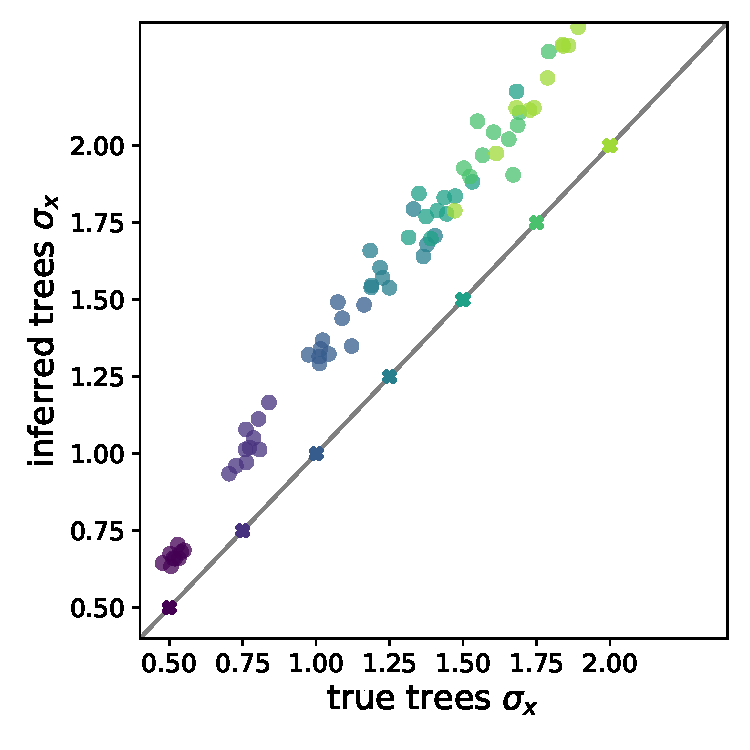
\includegraphics[height=0.32\linewidth, trim = {0cm 0 0cm 0}, clip]{plots/sim_sigmax_5numiter_100tCutoff.pdf}    
  };
  \node[left = 0cm of t100.north west, anchor = north west, yshift = -0.15cm] (A) {
    \textbf{A}
  };
  \node[above = -0.2cm of t100, xshift = 0.35cm] {time cutoff = $10^2$};

  \node[below = -0.2cm of t100] (t100y) {
    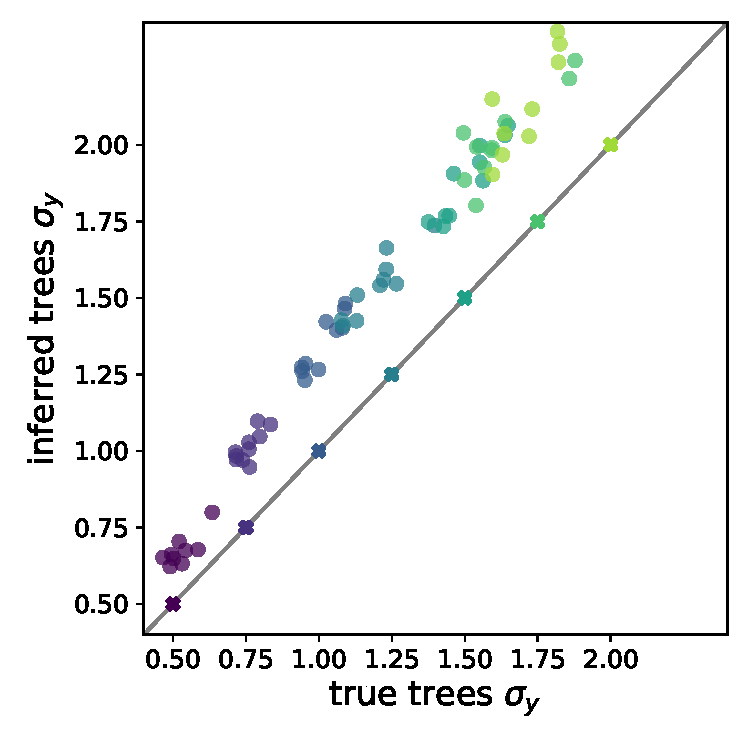
\includegraphics[height=0.32\linewidth, trim = {0cm 0 0cm 0}, clip]{plots/sim_sigmay_5numiter_100tCutoff.pdf}    
  };
    \node[below = -0.2cm of t100y] (t100p) {
    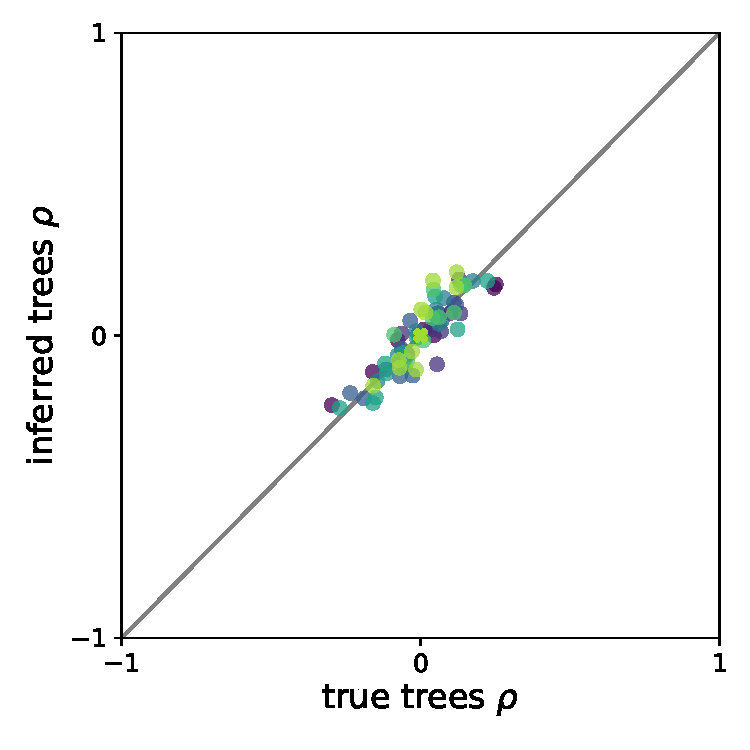
\includegraphics[height=0.32\linewidth, trim = {0cm 0 0cm 0}, clip]{plots/sim_rho_5numiter_100tCutoff.pdf}    
  };

  % tCutoff = $10^3$   
  \node[right = 0cm of t100] (t1000) {
    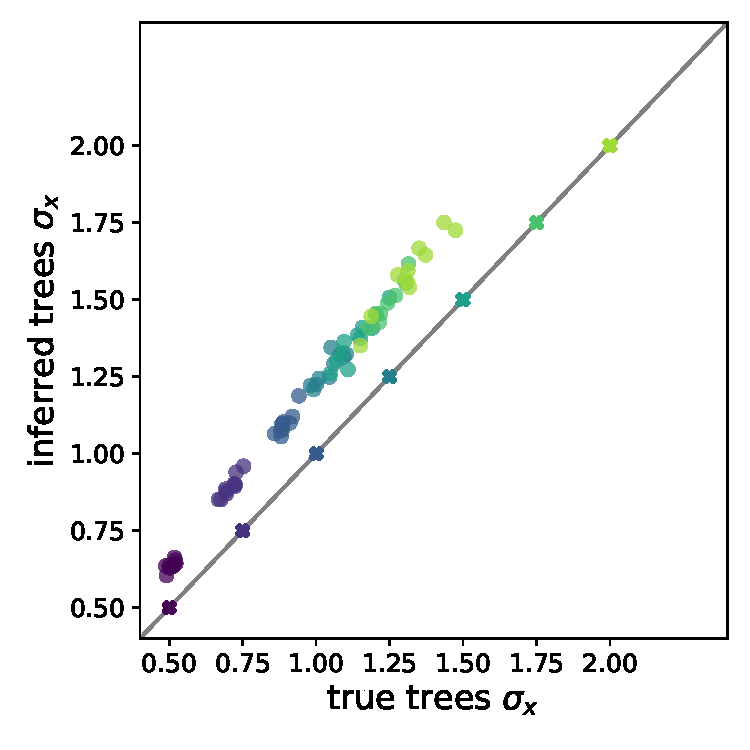
\includegraphics[height=0.32\linewidth, trim = {0cm 0 0cm 0}, clip]{plots/sim_sigmax_5numiter_1000tCutoff.pdf}    
  };
  \node[left = 0cm of t1000.north west, anchor = north west, yshift = -0.15cm] (B) {
    \textbf{B}
  };
  \node[above = -0.2cm of t1000, xshift = 0.35cm] {time cutoff = $10^3$};
  
  \node[below = -0.2cm of t1000] (t1000y) {
    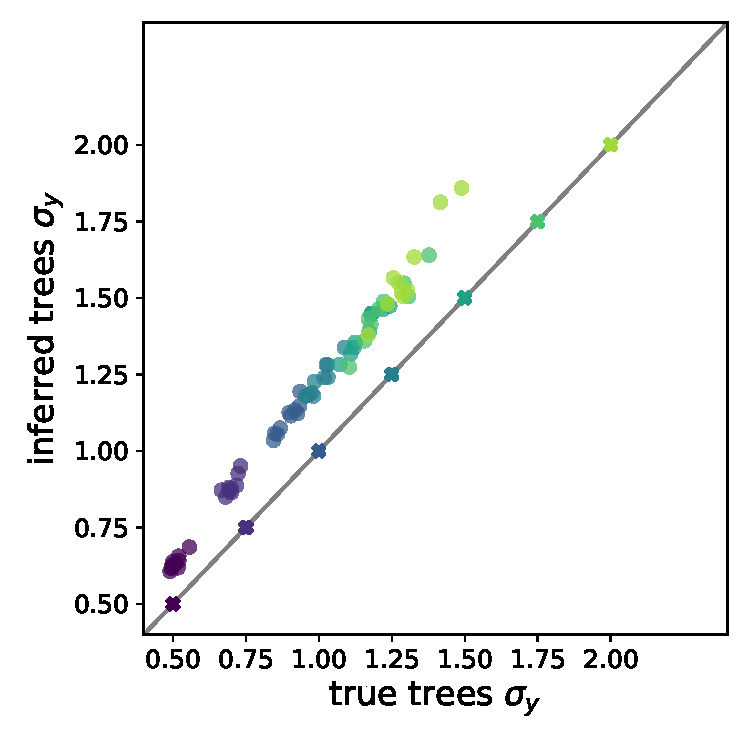
\includegraphics[height=0.32\linewidth, trim = {0cm 0 0cm 0}, clip]{plots/sim_sigmay_5numiter_1000tCutoff.pdf}    
  };
    \node[below = -0.2cm of t1000y] (t1000p) {
    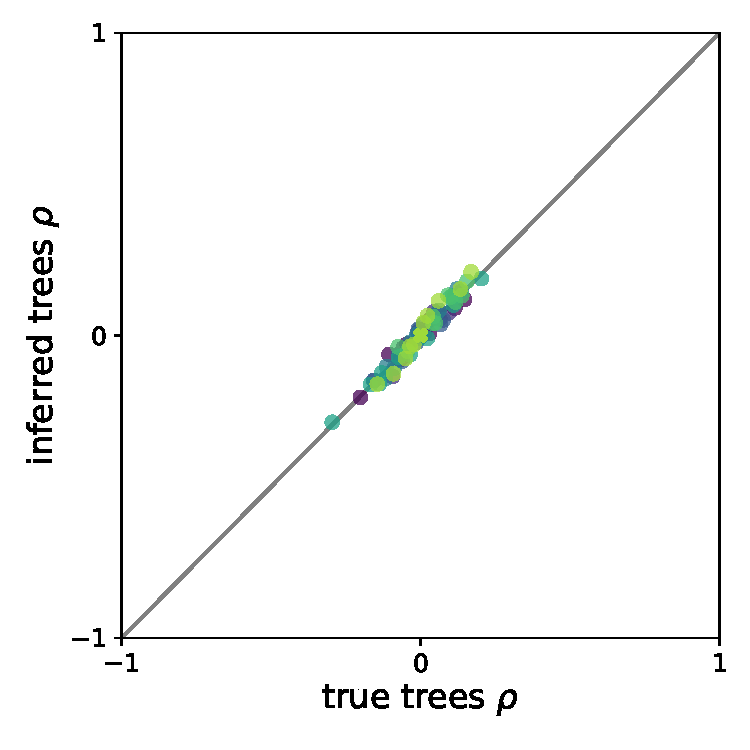
\includegraphics[height=0.32\linewidth, trim = {0cm 0 0cm 0}, clip]{plots/sim_rho_5numiter_1000tCutoff.pdf}    
  };
  
  % tCutoff = 10000
  \node[right = 0cm of t1000] (t10000) {
    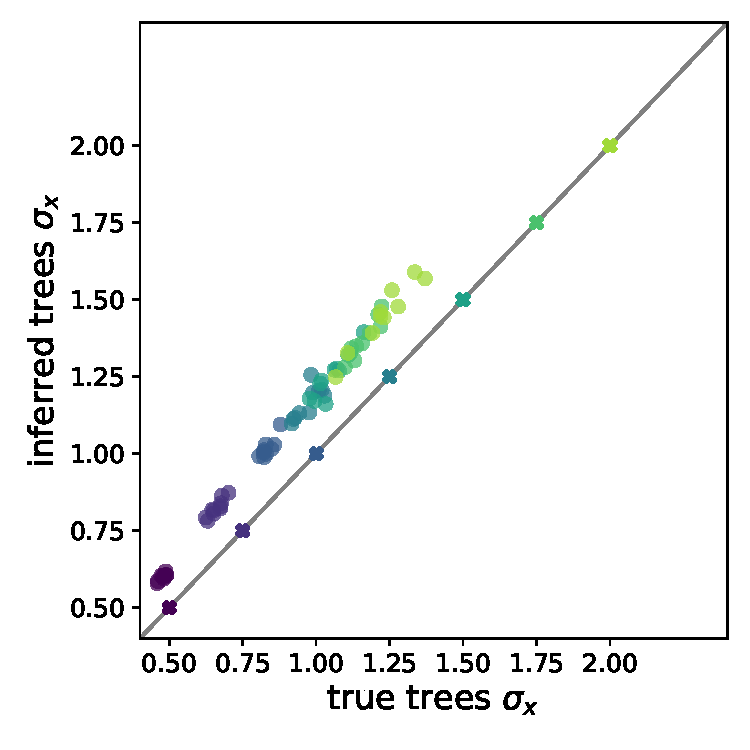
\includegraphics[height=0.32\linewidth, trim = {0cm 0 0cm 0}, clip]{plots/sim_sigmax_5numiter.pdf}    
  };
  \node[left = 0cm of t10000.north west, anchor = north west, yshift = -0.15cm] (C) {
    \textbf{C}
  };
  \node[above = -0.2cm of t10000, xshift = 0.35cm] {time cutoff = $10^4$};
  
  \node[below = -0.2cm of t10000] (t10000y) {
    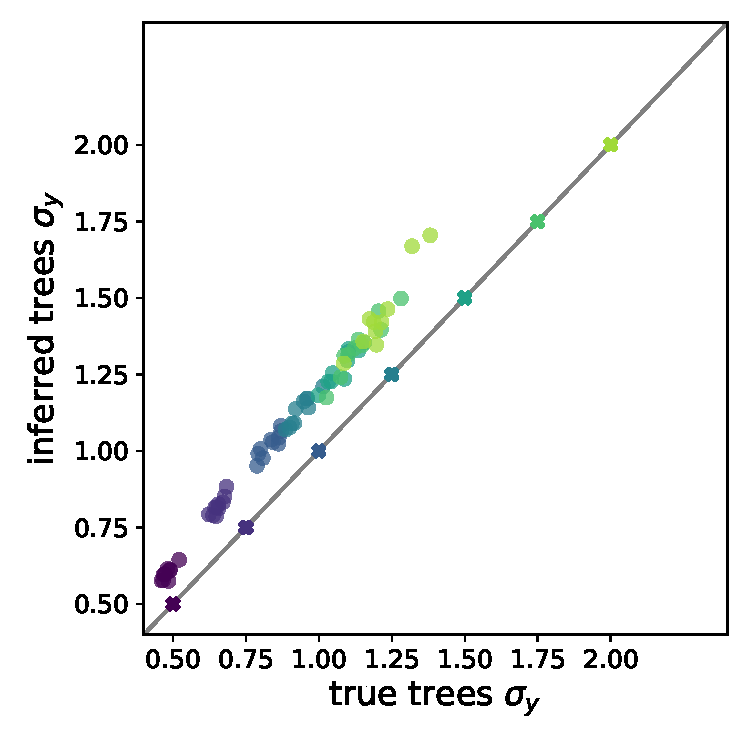
\includegraphics[height=0.32\linewidth, trim = {0cm 0 0cm 0}, clip]{plots/sim_sigmay_5numiter.pdf}    
  };
    \node[below = -0.2cm of t10000y] (t10000p) {
    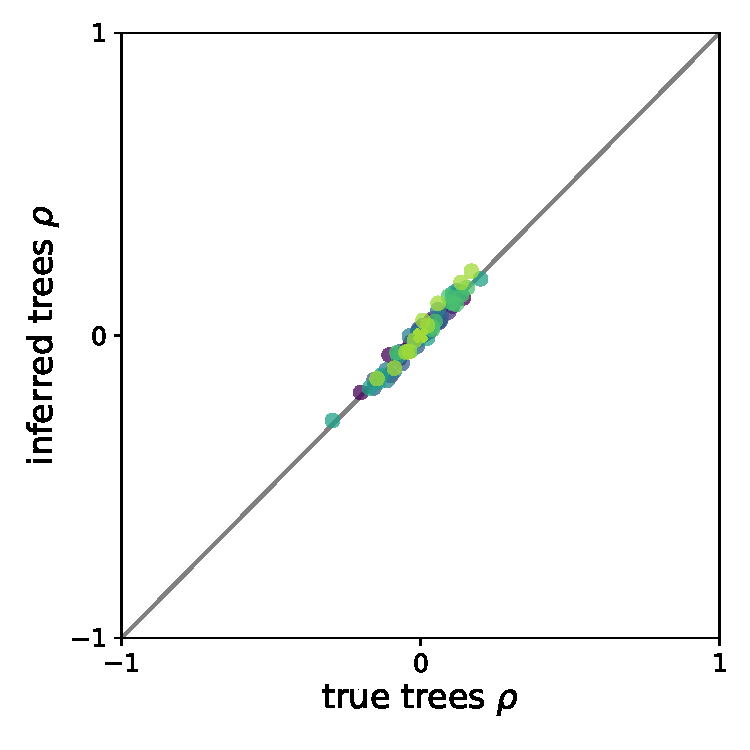
\includegraphics[height=0.32\linewidth, trim = {0cm 0 0cm 0}, clip]{plots/sim_rho_5numiter.pdf}    
  };
      
\end{tikzpicture}  

\end{center}

\caption{
\textbf{The effect of the time cutoff on dispersal estimates in one-epoch simulations.}
Panel \textbf{A} is as in the main text (Figure \ref{fig:sims}A), where we ignore everything beyond $10^2$ generations ago (and here we show dispersal along the y-axis in the correlation in x and y).
Panels \textbf{B} and \textbf{C} increase the time cutoff by one and two orders of magnitude, respectively.
Dispersal estimates shrink as the time cutoff grows because smaller dispersal rates make it more likely all lineages have remained within the finite habitat (with reflecting boundaries).
The variance in estimates seems to decline with the time cutoff, as larger cutoffs mean we use more information from the trees.
}

\label{fig:sup_sigma_corr_tcut}
\end{figure}

%%%%%%%%%%%%%%%%%%%%%%%%%%%%%%%%%%%%%%%%%%%%%%%%%

%%%%%%%%%%%%%%%%%%%%%%%%%%%%%%%%%%%%%%%%%%%%%%%%%
%simulation dispersal estimates -- effect of importance sampling
%%%%%%%%%%%%%%%%%%%%%%%%%%%%%%%%%%%%%%%%%%%%%%%%%

\begin{figure}[!htb]

\begin{center}

\begin{tikzpicture}[remember picture]

  % tCutoff = 100
  \node[] (t100) {
    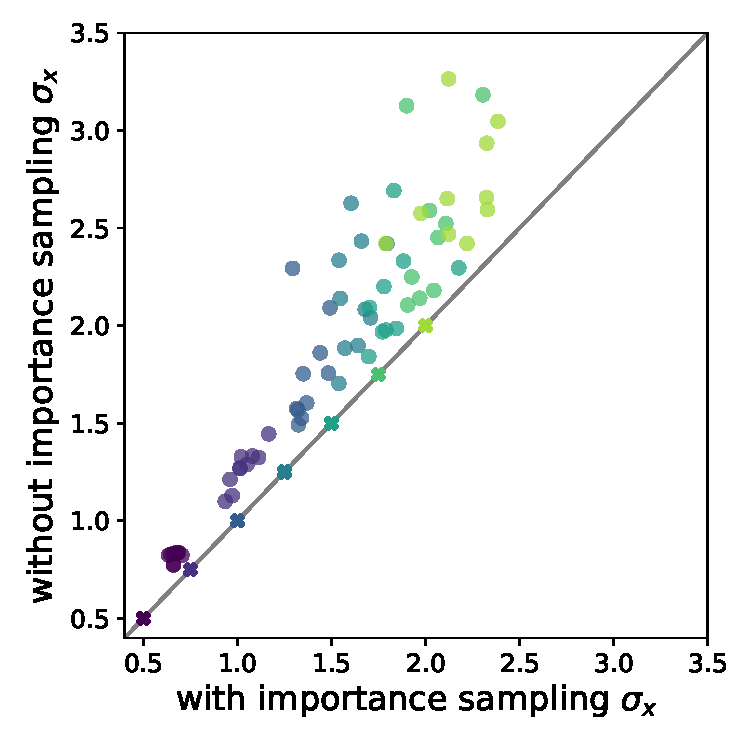
\includegraphics[height=0.32\linewidth, trim = {0cm 0 0cm 0}, clip]{plots/sim_sigmax_5numiter_100tCutoff_unimp.pdf}    
  };

  \node[above = -0.2cm of t100, xshift = 0.35cm] {time cutoff = $10^2$};

  \node[below = -0.2cm of t100] (t100y) {
    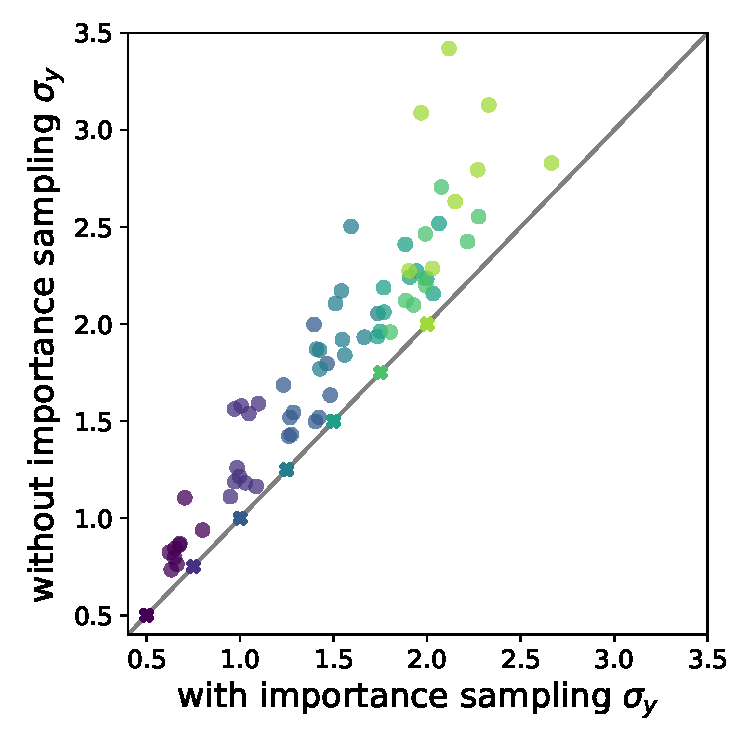
\includegraphics[height=0.32\linewidth, trim = {0cm 0 0cm 0}, clip]{plots/sim_sigmay_5numiter_100tCutoff_unimp.pdf}    
  };
    \node[below = -0.2cm of t100y] (t100p) {
    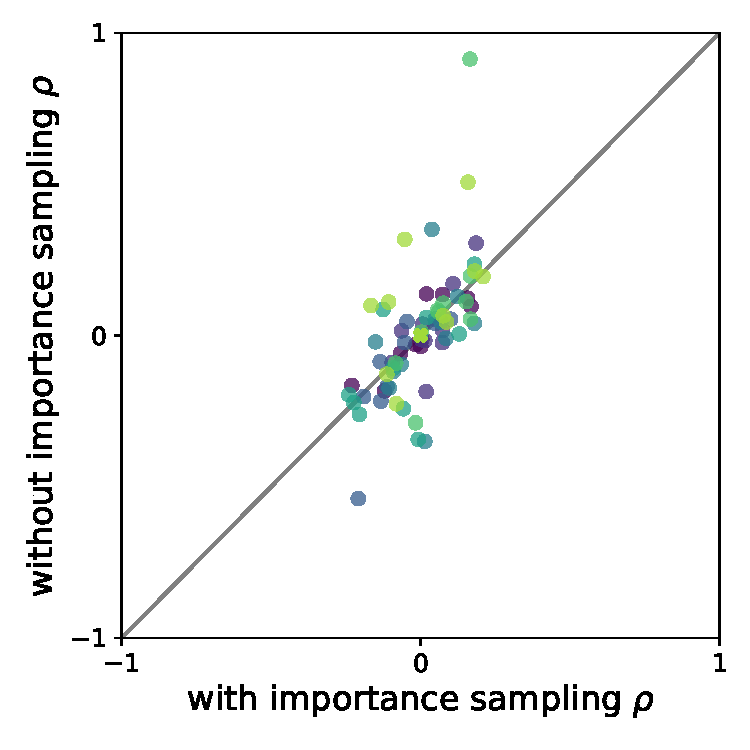
\includegraphics[height=0.32\linewidth, trim = {0cm 0 0cm 0}, clip]{plots/sim_rho_5numiter_100tCutoff_unimp.pdf}    
  };
      
\end{tikzpicture}  

\end{center}

\caption{
\textbf{The effect of importance sampling on dispersal estimates in one-epoch simulations.}
In all cases importance sampling leads to smaller overestimates of the simulated dispersal rate ($\sigma_x$ and $\sigma_y$) and generally exhibits lower variance in estimates across replicates (especially at high simulated dispersal rates).
The `without importance sampling' estimate comes from using only the first sample of branch lengths, while the `with importance sampling' estimate uses all 10 samples. 
}

\label{fig:sup_sigma_imp}
\end{figure}

%%%%%%%%%%%%%%%%%%%%%%%%%%%%%%%%%%%%%%%%%%%%%%%%%

%%%%%%%%%%%%%%%%%%%%%%%%%%%%%%%%%%%%%%%%%%%%%%%%%
%simulation dispersal estimates -- 2 epoch test
%%%%%%%%%%%%%%%%%%%%%%%%%%%%%%%%%%%%%%%%%%%%%%%%%

\begin{figure}[!htb]

\begin{center}

\begin{tikzpicture}[remember picture]

  % 2 epoch dispersal mcles: small -> small
  \node[] (plot11) {
    \includegraphics[height=0.32\linewidth, trim = {0cm 0 0cm 0}, clip]{plots/sim_2epoch_mcles_tsplits[0.25, 0.25].pdf}
  };
  \node[left = 0cm of plot11.north west, anchor = north west, yshift = -0.15cm] (letter) {
    \textbf{A}
  };
  \node[above = -0.2cm of plot11, xshift = 0.35cm, color=viridis_purple] {$\sigma_{x,\mathrm{ancient}} = 0.25$};
  
  % 2 epoch dispersal mcles: small -> large
  \node[right = 0cm of plot11] (plot12) {
    \includegraphics[height=0.32\linewidth, trim = {0cm 0 0cm 0}, clip]{plots/sim_2epoch_mcles_tsplits[0.5, 0.25].pdf}
  };
  \node[left = 0cm of plot12.north west, anchor = north west, yshift = -0.15cm] (letter) {
    \textbf{B}
  };
  \node[above = -0.2cm of plot12, xshift = 0.35cm, color=viridis_purple] {$\sigma_{x,\mathrm{ancient}} = 0.5$};
  \node[right = -0.2cm of plot12, xshift = 0.35cm, yshift = 1.5cm, rotate=270, color=viridis_blue] {$\sigma_{x,\mathrm{recent}} = 0.25$};
    
  % 2 epoch dispersal mcles: large -> small
  \node[below = 0cm of plot11] (plot21) {
    \includegraphics[height=0.32\linewidth, trim = {0cm 0 0cm 0}, clip]{plots/sim_2epoch_mcles_tsplits[0.25, 0.5].pdf}
  };
  \node[left = 0cm of plot21.north west, anchor = north west, yshift = -0.15cm] (letter) {
    \textbf{C}
  };
  
  % 2 epoch dispersal mcles: large -> large
  \node[right = 0cm of plot21] (plot22) {
    \includegraphics[height=0.32\linewidth, trim = {0cm 0 0cm 0}, clip]{plots/sim_2epoch_mcles_tsplits[0.5, 0.5].pdf}
  };
  \node[left = 0cm of plot22.north west, anchor = north west, yshift = -0.15cm] (letter) {
    \textbf{D}
  };
  \node[right = -0.2cm of plot22, xshift = 0.35cm, yshift = 1.5cm, rotate=270, color=viridis_blue] {$\sigma_{x,\mathrm{recent}} = 0.5$};    
  
\end{tikzpicture}  

\end{center}

\caption{
\textbf{Estimating two-epoch dispersal rates in simulations.}
Panels \textbf{B} and \textbf{D} are panels \textbf{B} and \textbf{C}, respectively, in Figure \ref{fig:sims}.
Panels \textbf{A} and \textbf{D} are simulated with a constant dispersal rate, $\sigma=0.25$ and $0.5$, respectively.
The coloured dots show the estimates for the recent and ancient epochs.
The grey dots show the estimates under a one-epoch model. 
}

\label{fig:sup_sigma_2epochs}
\end{figure}

%%%%%%%%%%%%%%%%%%%%%%%%%%%%%%%%%%%%%%%%%%%%%%%%%

%%%%%%%%%%%%%%%%%%%%%%%%%%%%%%%%%%%%%%%%%%%%%%%%%
%1001g two epoch dispersal%
%%%%%%%%%%%%%%%%%%%%%%%%%%%%%%%%%%%%%%%%%%%%%%%%%

\begin{figure}[!htb]
\begin{center}

%    \includegraphics[width=0.49\linewidth, trim = {0.25cm 0.5cm 0cm 0}, clip]{plots/1001G_2epoch_dispersal_no-japan.pdf}

\begin{tikzpicture}

  \node[] (A) {  
    \includegraphics[width=0.49\linewidth]{{plots/1001G_tCutoff10000_tsplits[10]_groupEurasia-no-Japan_mcle-dispersal.pdf}}
  };
  \node[anchor = north, xshift = 0cm, yshift = -0cm] at (A.north west) {
    \textbf{A}
  };  
  
  \node[below = 0cm of A] (B) {
    \includegraphics[width=0.49\linewidth]{{plots/1001G_tCutoff10000_tsplits[100]_groupEurasia-no-Japan_mcle-dispersal.pdf}}
  };
  \node[anchor = north, xshift = 0cm, yshift = -0cm] at (B.north west) {
    \textbf{B}
  };  

  \node[below = 0cm of B] (C) {
    \includegraphics[width=0.49\linewidth]{{plots/1001G_tCutoff10000_tsplits[1000]_groupEurasia-no-Japan_mcle-dispersal.pdf}} 
  };
  \node[anchor = north, xshift = 0cm, yshift = -0cm] at (C.north west) {
    \textbf{C}
  };  

\end{tikzpicture}

\end{center}

\caption{
\textbf{Dispersal rate estimates in \textit{Arabidopsis thaliana} under a two-epoch model.}
Like Figure \ref{fig:thal_sigma}B, but here we also show the (less likely) split times of (\textbf{B}) $10^2$ and (\textbf{C}) $10^3$.
}

\label{fig:thal_two_epoch_dispersal}
\end{figure}

%%%%%%%%%%%%%%%%%%%%%%%%%%%%%%%%%%%%%%%%%%%%%%%%%

%%%%%%%%%%%%%%%%%%%%%%%%%%%%%%%%%%%%%%%%%%%%%%%%%
%1001g three epoch dispersal%
%%%%%%%%%%%%%%%%%%%%%%%%%%%%%%%%%%%%%%%%%%%%%%%%%

\begin{figure}[!htb]
\begin{center}

\begin{tikzpicture}
  
  \node[] (A) {  
    \includegraphics[width=0.49\linewidth]{{plots/1001G_tCutoff10000_tsplits[10,100]_groupEurasia-no-Japan_mcle-dispersal.pdf}}
  };
  \node[anchor = north, xshift = 0cm, yshift = -0cm] at (A.north west) {
    \textbf{A}
  };  
  
  \node[below = 0cm of A] (B) {
    \includegraphics[width=0.49\linewidth]{{plots/1001G_tCutoff10000_tsplits[10,1000]_groupEurasia-no-Japan_mcle-dispersal.pdf}}
  };
  \node[anchor = north, xshift = 0cm, yshift = -0cm] at (B.north west) {
    \textbf{B}
  };  

  \node[below = 0cm of B] (C) {
    \includegraphics[width=0.49\linewidth]{{plots/1001G_tCutoff10000_tsplits[100,1000]_groupEurasia-no-Japan_mcle-dispersal.pdf}} 
  };
  \node[anchor = north, xshift = 0cm, yshift = -0cm] at (C.north west) {
    \textbf{C}
  };  

\end{tikzpicture}

\end{center}

\caption{
\textbf{Dispersal rate estimates in \textit{Arabidopsis thaliana} under a three-epoch model.}
Like Figure \ref{fig:thal_sigma}B, but here we also show the (less likely) split times of (\textbf{A}) [10,$10^2$] and (\textbf{C}) [$10^2$,$10^3$].
}

\label{fig:thal_three_epoch_dispersal}
\end{figure}

%%%%%%%%%%%%%%%%%%%%%%%%%%%%%%%%%%%%%%%%%%%%%%%%%%%%%%%

%%%%%%%%%%%%%%%%%%%%%%%%%%%%%%%%%%%%%%%%%%%%%%%%%
%1001g coalescence times%
%%%%%%%%%%%%%%%%%%%%%%%%%%%%%%%%%%%%%%%%%%%%%%%%%

\begin{figure}[!htb]
\begin{center}

\begin{tikzpicture}
  
  \node[] (A) {  
    \includegraphics[width=0.5\linewidth]{{1001G_coalescence-times_nodes[877,778]_chr2.pdf}}
  };
  \node[above = 0cm of A.north west, anchor = south west] () {
    \textbf{A}) accessions 9737 \& 9627 (chromosome 2)
  };
  
  \node[below = 0.5cm of A] (B) {  
    \includegraphics[width=0.5\linewidth]{{plots/1001G_coalescence-times_nodes[1044,1113]_chr2.pdf}}
  };
  \node[above = 0cm of B.north west, anchor = south west] () {
    \textbf{B}) accessions 9933 \& 10015 (chromosome 2)
  };

  \node[below = 0.5cm of B] (C) {  
    \includegraphics[width=0.5\linewidth]{{plots/1001G_coalescence-times_nodes[457,363]_chr5.pdf}}
  };
  \node[above = 0cm of C.north west, anchor = south west] () {
    \textbf{C}) accessions 7314 \& 6981 (chromosome 5)
  };

\end{tikzpicture}

\end{center}

\caption{
\textbf{Coalescence times between particular pairs of samples along a particular chromosome}.
Calculated using \texttt{tskit}'s \texttt{divergence()} function.
}
\label{fig:thal_coalescence_times}
\end{figure}

%%%%%%%%%%%%%%%%%%%%%%%%%%%%%%%%%%%%%%%%%%%%%%%%%%%%%%%

%%%%%%%%%%%%%%%%%%%%%%%%%%%%%%%%%%%%%%%%%%%%%%%%%
%1001g NA connections%
%%%%%%%%%%%%%%%%%%%%%%%%%%%%%%%%%%%%%%%%%%%%%%%%%

\begin{figure}[!htb]
\begin{center}

\begin{tikzpicture}
  
  \node[] (time1000) {
    \includegraphics[width=1\linewidth]{plots/1001g_NA-EUR.pdf}
  };
  
\end{tikzpicture}

\end{center}

\caption{
\textbf{Connecting the sample locations with the inferred present-day locations of the North American samples.}
Color indicates longitude of the inferred location.
See Figure \ref{fig:thal_NA} for more details.
}

\label{fig:thal_NA_connected}
\end{figure}

%%%%%%%%%%%%%%%%%%%%%%%%%%%%%%%%%%%%%%%%%%%%%%%%%%%%%%%

%%%%%%%%%%%%%%%%%%%%%%%%%%%%%%%%%%%%%%%%%%%%%%%%%
%1001g `Admixed'  genome displacements%
%%%%%%%%%%%%%%%%%%%%%%%%%%%%%%%%%%%%%%%%%%%%%%%%%

\begin{figure}[!htb]
\begin{center}

\begin{tikzpicture}
  
  \node[text width = \linewidth] (A) {  
    \includegraphics[width=1\linewidth]{{plots/1001G_genome-displacements_tsplits[10,100,1000]_node313_time10.pdf}}
  };
  \node[above = 0cm of A.north west, anchor = south west] () {
    accession 6830
  };
  
  \node[below = 0.5cm of A, text width = \linewidth] (B) {  
    \includegraphics[width=1\linewidth]{{plots/1001G_genome-displacements_tsplits[10,100,1000]_node408_time10.pdf}}
  };
  \node[above = 0cm of B.north west, anchor = south west] () {
    accession 7126
  };

  \node[below = 0.5cm of B, text width = \linewidth] (C) {  
    \includegraphics[width=1\linewidth]{{plots/1001G_genome-displacements_tsplits[10,100,1000]_node488_time10.pdf}}
  };
  \node[above = 0cm of C.north west, anchor = south west] () {
    accession 7394
  };

  \node[below = 0.5cm of C, text width = \linewidth] (D) {  
    \includegraphics[width=1\linewidth]{{plots/1001G_genome-displacements_tsplits[10,100,1000]_node881_time10.pdf}}
  };
  \node[above = 0cm of D.north west, anchor = south west] () {
    accession 9743
  };

  \node[below = 0.5cm of D, text width = \linewidth] (E) {  
    \includegraphics[width=1\linewidth]{{plots/1001G_genome-displacements_tsplits[10,100,1000]_node1044_time10.pdf}}
  };
  \node[above = 0cm of E.north west, anchor = south west] () {
    accession 9933
  };
  
  \node[below = 0.5cm of E, text width = \linewidth] (F) {  
    \includegraphics[width=1\linewidth]{{plots/1001G_genome-displacements_tsplits[10,100,1000]_node1095_time10.pdf}}
  };
  \node[above = 0cm of F.north west, anchor = south west] () {
    accession 9993
  };

\end{tikzpicture}

\end{center}

\caption{
\textbf{Genome-view of ancestral displacements for all 6 samples in Figure \ref{fig:thal_chr_displaced}.}
See Figure \ref{fig:thal_chr_displaced} for more details.
}
\label{fig:thal_admixed_genome_displacements}
\end{figure}

%%%%%%%%%%%%%%%%%%%%%%%%%%%%%%%%%%%%%%%%%%%%%%%%%%%%%%%

\end{document}